\input{setup.tex}

% Режим шаблона (должен быть включен один из трех)
\ВКРtrue
%\Практикаtrue
%\Курсоваяtrue

\newcommand{\Дисциплина}{-} % для курсовой
\newcommand{\КодСпециальности}{09.03.04} % Курсовая
\newcommand{\Специальность}{Программная инженерия} % Курсовая
\newcommand{\Тема}{Распределенная поисковая система для Интернета} % ВКР Курсовая
\newcommand{\ТемаВтораяСтрока}{-}
\newcommand{\ГдеПроводитсяПрактика}{ООО «МЦОБ. Онлайн-сервисы»} % для практики
\newcommand{\РуководительПрактПредпр}{Гавришко А. М.} % для практики
\newcommand{\ДолжнРуководительПрактПредпр}{генеральный директор} % для практики
\newcommand{\РуководительПрактУнивер}{Чаплыгин А. А.} % для практики
\newcommand{\ДолжнРуководительПрактУнивер}{к.т.н. доцент} % для практики
\newcommand{\Автор}{И. Р. Скулков}
\newcommand{\АвторРод}{Скулкова И.Р.}
\newcommand{\АвторПолностьюРод}{Скулкова Ильи Руслановича} % для практики
\newcommand{\Шифр}{20-06-0155}
\newcommand{\Курс}{4 } % для практики
\newcommand{\Группа}{ПО-01б}
\newcommand{\Руководитель}{А. А. Чаплыгин} % для ВКР и курсовой
\newcommand{\Нормоконтроль}{А. А. Чаплыгин} % для ВКР
\newcommand{\ЗавКаф}{А. В. Малышев} % для ВКР
\newcommand{\ДатаПриказа}{«04» апреля 2024~г.} % для ВКР
\newcommand{\НомерПриказа}{1620-с} % для ВКР
\newcommand{\СрокПредоставления}{«11» июня 2024~г.} % для ВКР, курсового

\begin{document}
\maketitle
\ifПрактика{}\else{
   \newsection
\begin{center}
\large\textbf{Минобрнауки России}

\large\textbf{Юго-Западный государственный университет}
\vskip 1em
\normalsize{Кафедра программной инженерии}
\vskip 1em

\begin{flushright}
\begin{tabular}{p{.4\textwidth}}
\centrow УТВЕРЖДАЮ: \\
\centrow Заведующий кафедрой \\
\hrulefill \\
\setarstrut{\footnotesize}
\centrow\footnotesize{(подпись, инициалы, фамилия)}\\
\restorearstrut
«\underline{\hspace{1cm}}»
\underline{\hspace{3cm}}
20\underline{\hspace{1cm}} г.\\
\end{tabular}
\end{flushright}
\end{center}
\section*{ЗАДАНИЕ НА ВЫПУСКНУЮ КВАЛИФИКАЦИОННУЮ РАБОТУ
  ПО ПРОГРАММЕ БАКАЛАВРИАТА}
{\parindent0pt
  Студента \АвторРод, шифр\ \Шифр, группа \Группа
  
1. Тема «\Тема\ \ТемаВтораяСтрока» утверждена приказом ректора ЮЗГУ от \ДатаПриказа\ № \НомерПриказа.

2. Срок предоставления работы к защите \СрокПредоставления

3. Исходные данные для создания программной системы:

3.1. Перечень решаемых задач:}



3.2. Входные данные и требуемые результаты для программы:}





4. Содержание работы (по разделам):

4.1. Введение

4.2. Анализ предметной области

4.6. Заключение

4.7. Список использованных источников

5. Перечень графического материала:

\begin{tabular}{@{}p{6.8cm}C{3.8cm}C{4.8cm}}
Руководитель ВКР & \lhrulefill{\fill} & \fillcenter\Руководитель\\
\setarstrut{\footnotesize}
& \footnotesize{(подпись, дата)} & \footnotesize{(инициалы, фамилия)}\\
\restorearstrut
Задание принял к исполнению & \lhrulefill{\fill} & \fillcenter\Автор\\
\setarstrut{\footnotesize}
& \footnotesize{(подпись, дата)} & \footnotesize{(инициалы, фамилия)}\\
\restorearstrut
\end{tabular}
}

   \abstract{РЕФЕРАТ}

Объем работы равен \formbytotal{lastpage}{страниц}{е}{ам}{ам}. Работа содержит \formbytotal{figurecnt}{иллюстраци}{ю}{и}{й}, \formbytotal{tablecnt}{таблиц}{у}{ы}{}, \arabic{bibcount} библиографических источников и \formbytotal{числоПлакатов}{лист}{}{а}{ов} графического материала. Количество приложений – 2. Графический материал представлен в приложении А. Фрагменты исходного кода представлены в приложении Б.

Перечень ключевых слов: поиск, индекс, ранг, система, распределенность, масштабирование, архитектура, тестирование, Интернет, библиотека, компонент, класс, диаграмма, API, веб-сайт.

Объектом разработки является распределенная поисковая система для Интернета.

Целью выпускной квалификационной работы является разработка эффективного инструмента для нахождения наиболее релевантных WEB-документов по пользовательскому запросу.

В процессе создания распределенной системы были выделены основные логические самостоятельные компоненты, реализованные в парадигме ООП. Для высокой производительности основная часть системы была реализована с помощью языка C++. Для уменьшения связанности и повышения гибкости был использован брокер сообщений RabbitMQ. Также была применена такая технология баз данных, как Postgres, для хранения и манипулирования большими объемами информации в рамках системы. Дополнительно были использованы различные вспомогательные инструменты для работы с асинхронностью, многопоточностью, логгированием и анализом текста разных типов, что сделало систему более модульной и поддерживаемой. Были разработаны следующие компоненты: поисковый робот, индексатор, поисковик, веб-сайт и сборщик журналируемой информации.

Каждый из компонентов удачно прошел системное тестирование, что говорит о достаточно высокой надежности системы.

\selectlanguage{english}
\abstract{ABSTRACT}
  
The volume of work is \formbytotal{lastpage}{page}{}{s}{s}. The work contains \formbytotal{figurecnt}{illustration}{}{s}{s}, \formbytotal{tablecnt}{table}{}{s}{s}, \arabic{bibcount} bibliographic sources and \formbytotal{числоПлакатов}{sheet}{}{s}{s} of graphic material. The number of applications is 2. The graphic material is presented in annex A. The layout of the site, including the connection of components, is presented in annex B.

The list of keywords: search, index, rank, system, distribution, scaling, architecture, testing, Internet, library, component, class, diagram, API, website.

The object of the development is a distributed search engine for the Internet.

The purpose of the final qualification work is to develop an effective tool for finding the most relevant WEB documents for a user request.

In the process of creating a distributed system, the main logical independent components implemented in the OOP paradigm were identified. For high performance, the main part of the system was implemented using the C++ language. The RabbitMQ message broker was used to reduce connectivity and increase flexibility. Database technology such as Postgres was also used to store and manipulate large amounts of information within the system. Additionally, various auxiliary tools were used to work with asynchrony, multithreading, logging and text analysis of various types, which made the system more modular and supported. The following components have been developed: a search robot, an indexer, a search engine, a website and a collector of journaled information.

Each of the components has successfully passed system testing, which indicates a fairly high reliability of the system.
\selectlanguage{russian}
}\fi
\tableofcontents
\newsection
\section*{ОБОЗНАЧЕНИЯ И СОКРАЩЕНИЯ}

БД -- база данных.

ИС -- информационная система.

ИПС -- информационно-поисковая система.

ИПВС -- информационно-поисковая веб-система.

ИТ -- информационные технологии. 

КТС -- комплекс технических средств.

ОМТС -- отдел материально-технического снабжения. 

ПО -- программное обеспечение.

РП -- рабочий проект.

СУБД -- система управления базами данных.

ТЗ -- техническое задание.

ТП -- технический проект.

UML (Unified Modelling Language) -- язык графического описания для объектного моделирования в области разработки программного обеспечения.

REP (Robots Exclusion Protocol) -- соглашение, предотвращающее доступ сканирующих веб-роботов ко всему веб-сайту или его части, которые в противном случае доступны для публичного просмотра. 

HPC (High-Performance Cluster) -- тип кластера, ориентированный на высокопроизводительные вычисления.
\ifПрактика{}\else{\section*{ВВЕДЕНИЕ}
\addcontentsline{toc}{section}{ВВЕДЕНИЕ}

Интернет -- всемирная система объединенных компьютерных сетей для хранения и передачи информации, построенная на стеке протоколов TCP/IP. На его основе работает Всемирная паутина (WWW,  web) -- распределенная система, предоставляющая доступ к связанным между собой документам.  Большинство ресурсов Всемирной паутины основано на технологии гипертекста. Гипертекстовые документы, размещаемые во Всемирной паутине, называются веб-страницами.

Веб-страницы часто содержат очень полезную для той или иной деятельности информацию, но ввиду огромного их количества возникает проблема эффективности ориентирования между ними. Поэтому из нее вполне закономерно следует задача о возможности подбора наиболее подходящих страниц, где фильтром будет выступать пользовательский текстовый запрос. Именно эту задачу и решают поисковые системы.

\emph{Цель настоящей работы} – разработка распределенной поисковой системы для Интернета. Для достижения поставленной цели необходимо решить \emph{следующие задачи:}
\begin{itemize}
\item провести анализ предметной области;
\item разработать концептуальную модель распределенной поисковой системы;
\item спроектировать компоненты распределенной поисковой системы и их взаимодействие между собой;
\item реализовать каждый из компонентов распределенной поисковой системы;
\item разработать поисковый web-сайт.
\end{itemize}

\emph{Структура и объем работы.} Отчет состоит из введения, 4 разделов основной части, заключения, списка использованных источников, 2 приложений. Текст выпускной квалификационной работы равен \formbytotal{page}{страниц}{е}{ам}{ам}.

\emph{Во введении} сформулирована цель работы, поставлены задачи разработки, описана структура работы, приведено краткое содержание каждого из разделов.

\emph{В первом разделе} на стадии описания технической характеристики предметной области приводится сбор информации об устройстве работы современных поисковых систем.

\emph{Во втором разделе} на стадии технического задания приводятся требования к распределенной поисковой системе.

\emph{В третьем разделе} на стадии технического проектирования представлены проектные решения для распределенной поисковой системы.

\emph{В четвертом разделе} приводится список классов и их методов, использованных при разработке распределенной поисковой системы, производится её системное тестирование.

В заключении излагаются основные результаты работы, полученные в ходе разработки.

В приложении А представлен графический материал.
В приложении Б представлены фрагменты исходного кода. }\fi
\section{Анализ предметной области}
\subsection{Понятие информационного поиска}

Информационный поиск (ИП) - это процесс поиска в большой коллекции (хранящейся, как правило, в памяти компьютеров) некоего неструктурированного материала (документа), удовлетворяющего информационные потребности [1]. Под словом "<неструктурированность"> подразумевается свойство данных, при котором они не имеют семанически очевидной и тривиально реализуемой на компьютере структуры.

В общем случае ИП состоит из следующих этапов:
\begin{itemize}
\item определение информационной потребности и формулировка информационного запроса;
\item определение совокупности возможных держателей информационных источников;
\item извлечение информации из выявленных информационных массивов;
\item ознакомление с полученной информацией и оценка результатов поиска.
\end{itemize}

Можно выделить следующие виды ИП:
\begin{itemize}
\item полнотекстовый поиск -- поиск по всему содержимому документа;
\item поиск по метаданным -- поиск по некоторому множеству атрибутов документа, поддерживаемым системой -- название документа, дата создания, автор, размер и т.д;
\item поиск изображений -- поиск по содержанию изображения путем распознавания содержания фотографии, результат которого представляется похожими изображениями.
\end{itemize}
 
\subsection{История развития информационно-поисковых систем}
На раннем этапе развития сети Интернет Тим Бернерс-Ли вручную поддерживал список веб-серверов, размещенных на сайте ЦЕРН (Европейский Центр ядерных исследований). Однако с ростом числа сайтов поддерживать такой список становилось сложнее. Более того, многократно увеличивалась сложность ручного поиска нужной информации, которая теоретически могла быть частично представлена на большом множестве сайтов. Эти обстоятельства во многом стали предпоссылками к созданию автоматизированных систем поиска.

Первой компьютерной программой для поиска в Интернете была программа Арчи (от англ. archie -- архив без буквы "<в">). Программа скачивала списки всех файлов со всех доступных FTP (File Transfer Protocol) -- серверов и строила базу данных, в которой можно было выполнять поиск по именам файлов. Недостатком данной системы можно считать отсутствие механизмов индексирования содержимого файлов, так как объем данных был настолько мал, что все можно было легко находить вручную.

В дальнейшем было создано несколько для того времени новых поисковых программ, которые индексировали заголовки документов и предоставляли возможность поиска по ключевым словами из них. Однако до лета 1993 года еще не было ни одной системы для поиска на WWW-пространстве. Только к июню 1993 года был создан вероятно первый поисковый робот "<World Wide Web Wanderer">, написанный на языке Perl. Цель этого робота состояла в том, чтобы измерить размер всемирной паутины и найти все веб-страницы, содержащие слова из запроса.

В свою очередь, созданную позднее систему JumpStation можно считать первой, которая во многом похожа на современные системы поиска. В её функциональность входил поиск веб-страниц и построение индексов с помощью поисковых роботов и предоставление веб-формы в качестве интерфейса для формулирования поисковых запросов. Но несмотря на все достоинства, поиск в такой системе был возможен только по названиям и заголовкам веб-страниц ввиду ограниченности ресурсов компьютеров.

Первой полнотекстовой индексирующей ресурсы при помощи робота поисковой системой стала система "<WebCrawler">, запущенная в 1994 году. Её ключевым преимуществом перед предшествующими системами было то, что она позволяла пользователям проводить поиск по любым словам, расположенным на любой веб-странице, что стало с тех пор де-факто стандартом для большинства поисковых систем.

Вскоре появилось множество других конкурирующих поисковых систем и начались первые попытки интеграции поисковых систем и веб-браузеров. В дальнейшем поисковые системы стали продавать первые места в результатах поиска отдельным компаниям.

Впоследствии мировой сегмент использования систем веб-поиска был неравномерно распределен между Yahoo!, Microsoft Bing, Baidu и Google в пользу последней. На российском сегменте популярностью обзавелись Yandex, Mail.ru и Rambler.

\subsection{Понятие и принципы работы информационно-поисковой системы}

Информационно-поисковая система (ИПС) - набор взаимосвязанных программных компонентов, реализующих специальные алгоритмы по поиску, обработке и хранению данных некоторого информационного пространства, целью которого является предоставление пользователю возможности быстрого доступа к необходимой информации при помощи поиска в обширной коллекции документов [2].

Как правило, пользователь взаимодействует с ИПС путем создания запроса, где:
\begin{itemize}
\item запрос -- это формализованный способ выражения информационных потребностей пользователем системы, в котором может использоваться как специальный язык поисковых запросов, так и ествественный язык;
\item объект запроса -- это информационная сущность, которая представлена в ИПС в виде некоторого суррогата.
\end{itemize}

Современные версии ИПС в общем случае работают на следующих принципах:
\begin{itemize}
\item выявляется множество документов, содержание которых будет учитываться при обработке запросов пользователя. В случае динамического изменения коллекции документов или их содержимого предусматриваются механизмы поиска и добавления новых экземпляров и их индексации соответственно;
\item документы, доступные для обработки ИПС, подвергаются индексированию. Это процесс обработки коллекции документов, в ходе которого их содержимое сжимается и преобразуется в некоторую структуру данных, называемую индексом, таким образом, чтобы в дальнейшем ИПС могла обеспечить эффективный по времени поиск документов, удовлетворяющих пользовательскому запросу. Индекс может содержать в себе несколько гранулярных структур данных, предназначенных для решения конкретных поисковых задач. В крупномасштабных ИПС индексы, как правило, имеют распределенное представление в виду невозможности хранения физически всей информации на одном сервере;
\item производится дополнительная обработка запросов пользователя. В случае ИПС с конкретными языками запросов проводится проверка запроса на соответствие синтаксису. Также система может обрабатывать запросы с элементами регулярных выражений, вносить орфографические или фонетические исправления в запрос, информируя об этом пользователя. В результате таких действий один пользовательский запрос может быть разбит на некоторое множество производных, с целью выдачи максимально полного ответа;
\item используются специальные методы первичной обработки текста, чтобы привести его к виду, наиболее приспособленному для обработки без существенной потери смысловых характеристик;
\item собираются статистические данные. Они нужны ИПС, основывающимся на вероятностных моделях обработки информации и использующих различные технологии машинного обучения, чтобы система имела возможность в режиме онлайн улучшать качество своей работы. Также они могут послужить для оценки качества работы системы и нахождения её уязвимых мест.
\end{itemize}

Все ИПС можно разделить на несколько видов:
\begin{itemize}
\item системы, использующие поисковых роботов. Роботы (краулеры, от англ. crawler) занимаются исследованием информационного пространства ИПС (как правило, через сеть), чтобы поддерживать актуальное множество документов. В индексе хранится большой архив приближенных к ним копий. Большинство поисковых систем являются системами данного типа;
\item системы, управляемые человеком. Эти поисковые системы получают готовые списки документов. Каталог содержит адрес, заголовок и краткое описание документа. Каталог ресурсов ищет результаты только из описания, представленных ему создателями документа. Достоинство каталогов в том, что все ресурсы проверяются вручную, следовательно, и качество контента будет лучше по сравнению с результатами, полученными системой первого типа автоматически. Но есть и недостаток — обновление данных каталогов выполняется вручную и может существенно отставать от реального положения дел. Известный пример такой системы - каталог Yahoo;
\item гибридные системы. Такие системы сочетают в себе функции систем как с использованием поисковых роботов, так и управляемых человеком. Примеры систем: Google, Yahoo;
\item мета-системы. Они объединяют и ранжируют результаты сразу из нескольких поисковиков. Эти поисковые системы были полезны, когда у каждой поисковой системы был уникальный индекс, и поисковые системы были менее «умными». Поскольку сейчас поиск намного улучшился, потребность в них уменьшилась. Пример такой системы - MSN Search.
\end{itemize}

Для оценки работы ИПС в основном используются следующие метрики:
\begin{itemize}
\item точность (по англ. precision) -- определяется как отношение числа релеватных документов, найденных ИПС, к общему числу найденных документов.

\begin{equation}
P = \frac{| D_{rel} \bigcap D_{retr} |}{| D_{retr} |},
\end{equation} где $D_{rel}$ -- множество релевантных документов из базы данных, а $D_{retr}$ -- множество документов, найденных системой;
\item полнота (по англ. recall) -- определяется как отношение числа найденных релевантных документов, найденных ИПС, к общему числу релевантных документов из базы данных.
\begin{equation}
R = \frac{| D_{rel} \bigcap D_{retr} |}{| D_{rel} |},
\end{equation} где $D_{rel}$ -- множество релевантных документов из базы данных, а $D_{retr}$ -- множество документов, найденных системой. 
\end{itemize}

\subsection{Основные компоненты информационно-поисковых систем на WWW-пространстве}

Информационно-поисковая система на WWW-пространстве (ИПВС) - разновидность ИПС, которая в качестве целевого информационного пространства использует WWW-пространство (веб-пространство). Как правило, ИПВС относится к виду ИПС с поисковым роботом или же является гибридной. Также в большинстве современных ИПВС реализованы полнотекстовый поиск и поиск по изображениям.

В настоящее время подобного рода ИПС пользуются колоссальным спросом. Целью таких ИПС является предоставление пользователям возможности быстрого доступа к информации различных сайтов и в особенности тех, которые пользуются относительной популярностью и доверием.

ИПВС не перестают ориентироваться на потребности конечных пользователей. Их можно разделить на следующие категории:
\begin{itemize}
\item информационные потребности, цель которых найти общую информацию по широкой теме. Обычно вся информация не находится на одной веб-странице, поэтому пользователи посещают несколько ресурсов из результатов поиска. В таком случае оптимально, чтобы полнота ответа на этот запрос была максимальной;
\item навигационные запросы отражают желание найти конкретный веб-сайт или домашнюю страницу. Пользователь в этом случае ожидает, что среди первых результатов должен быть желаемый ресурс, при этом его не интересуют другие возможные результаты запроса. В таком случае оптимально, чтобы точность ответа на этот запрос была максимальной;
\item транзакционные запросы предшествуют совершению транзакций в вебе, например покупке товара или загрузке файла. В таких случаях ИПВС должна возвращать в качестве результатов список сервисов, предоставляющих интерфейс для выполнения таких транзакций. В этом случае оптималальна полнота ответа на запрос без существенных потерь в точности.
\end{itemize}

В соответствие с определением можно заключить, что документной единицей такой системы является веб-страница некоторого сайта. Страницы могут быть двух видов:
\begin{itemize}
\item статической, содержание которой не меняется от запроса к запросу;
\item динамической, содержание которых обычно автоматически генерируется сервером приложения в ответ на запрос к базе данных.
\end{itemize}

Любая веб-страница представлена в формате HTML, отдельно в котором представляются текст, изображения и гиперссылки, часто перенаправляющие на другие веб-страницы, которые могут быть ресурсами как текущего домена, так и абсолютно другого. По этой причине часто для моделирования работы в веб-пространстве его представляют в виде ориентированного графа, где вершины -- статические HTML-документы, а ребра -- гиперссылки.

На рисунке 1.1 изображены основные структурные компоненты ИПВС, которые включают в себя:
\begin{itemize}
\item поисковый робот -- программный модуль по сбору максимально большого множества полезных веб-страниц вместе со ссылками, которые их объединяют, для их дальнейшего индексирования и поддержки функционирования ИПВС. Такое поведение также называют обходом веба (по англ. web crawling). Поисковый робот начинает работу с одного или нескольких URL, образующих начальное множество (по англ. seed set). Он извлекает URL из этого множества, а затем загружает по нему веб-страницу. После этого выбранная страница обрабатывается и из нее c помощью навигации по соответствующим метатегам извлекаются текст и ссылки  (каждая из них указывает на другой URL). Извлеченный текст передается индексатору (другому компоненту ИПВС, занимающемуся индексированием документов). Извлеченные ссылки передаются очереди на скачивание URL, состоящей из URL, соответствующих страницам, которые должны быть загружены поисковым роботом. В самом начале очередь на скачивание URL содержит начальное множество; как только страница выбрана, ее адрес удаляется из очереди на скачивание URL. Данный процесс можно рассматривать как обход в ширину веб-графа;
\item индексатор -- программный модуль, реализующий собственные алгоритмы по лексическому, морфологическому разбору текста и хранению данных для последующего эффективного поиска, которые анализируют содержимое веб-страницы, предварительно разбив его на части. Как правило, на начальном этапе проходит первичная обработка текста, целью которой является разбиение сырого текста на поток нормализованных токенов. Далее поток записывается в индексные структуры данных, сжимается и сохраняется на серверах баз данных для дальнейшего использования;
\item поисковый сервис (поисковик) -- программный модуль, непосредственно обрабатывающий пользовательские запросы с помощью построенного индекса документов. Взаимодействие с пользователем происходит через специальную поисковую веб-страницу путем ввода запроса. В общем случае поисковик имеет следующий алгоритм действий [3]:
\begin{enumerate}
\item Поисковик получает входящий пользовательский запрос.
\item Производит первичную текстовую обработку запроса, трансформируя его в поток нормализованных токенов.
\item С возможным участием пользователя исправляет орфографические или фонетические ошибки в запросе.
\item В случае наличия элементов регулярных выражений разбивает запрос на эквивалентное множество простых запросов без регулярных выражений.
\item С целью обработать возможные многословные выражения также разбивает каждый простой запрос на несколько таких, в которых предполагаются лишь односложные токены.
\item Начинает обрабатывать сформировавшееся конечное множество простых запросов.
\item Для каждого запроса обращается к базам данных, декодирует индексные файлы, по ним находит множество документов, соответствующих данному запросу, проводит ранжирование на основании разных частотных критериев и сортирует по убыванию коэффициента получившегося ранга документа.
\item В случае, если ранг документа выше определенного значения, то с помощью индекса вычленяются соответствующие фрагменты текста, в которых были найдены вхождения входных токенов (по англ. snippets) и документ со всей дополнительной информацией попадает в выборку результатов.
\item Объединяет результаты для всех простых запросов в один большой список, также отсортированный по рангу документов.
\item Возвращает информацию о результатах поиска в заданном пользователем диапазоне.
\end{enumerate}
\end{itemize}

\begin{figure}[H]
\center{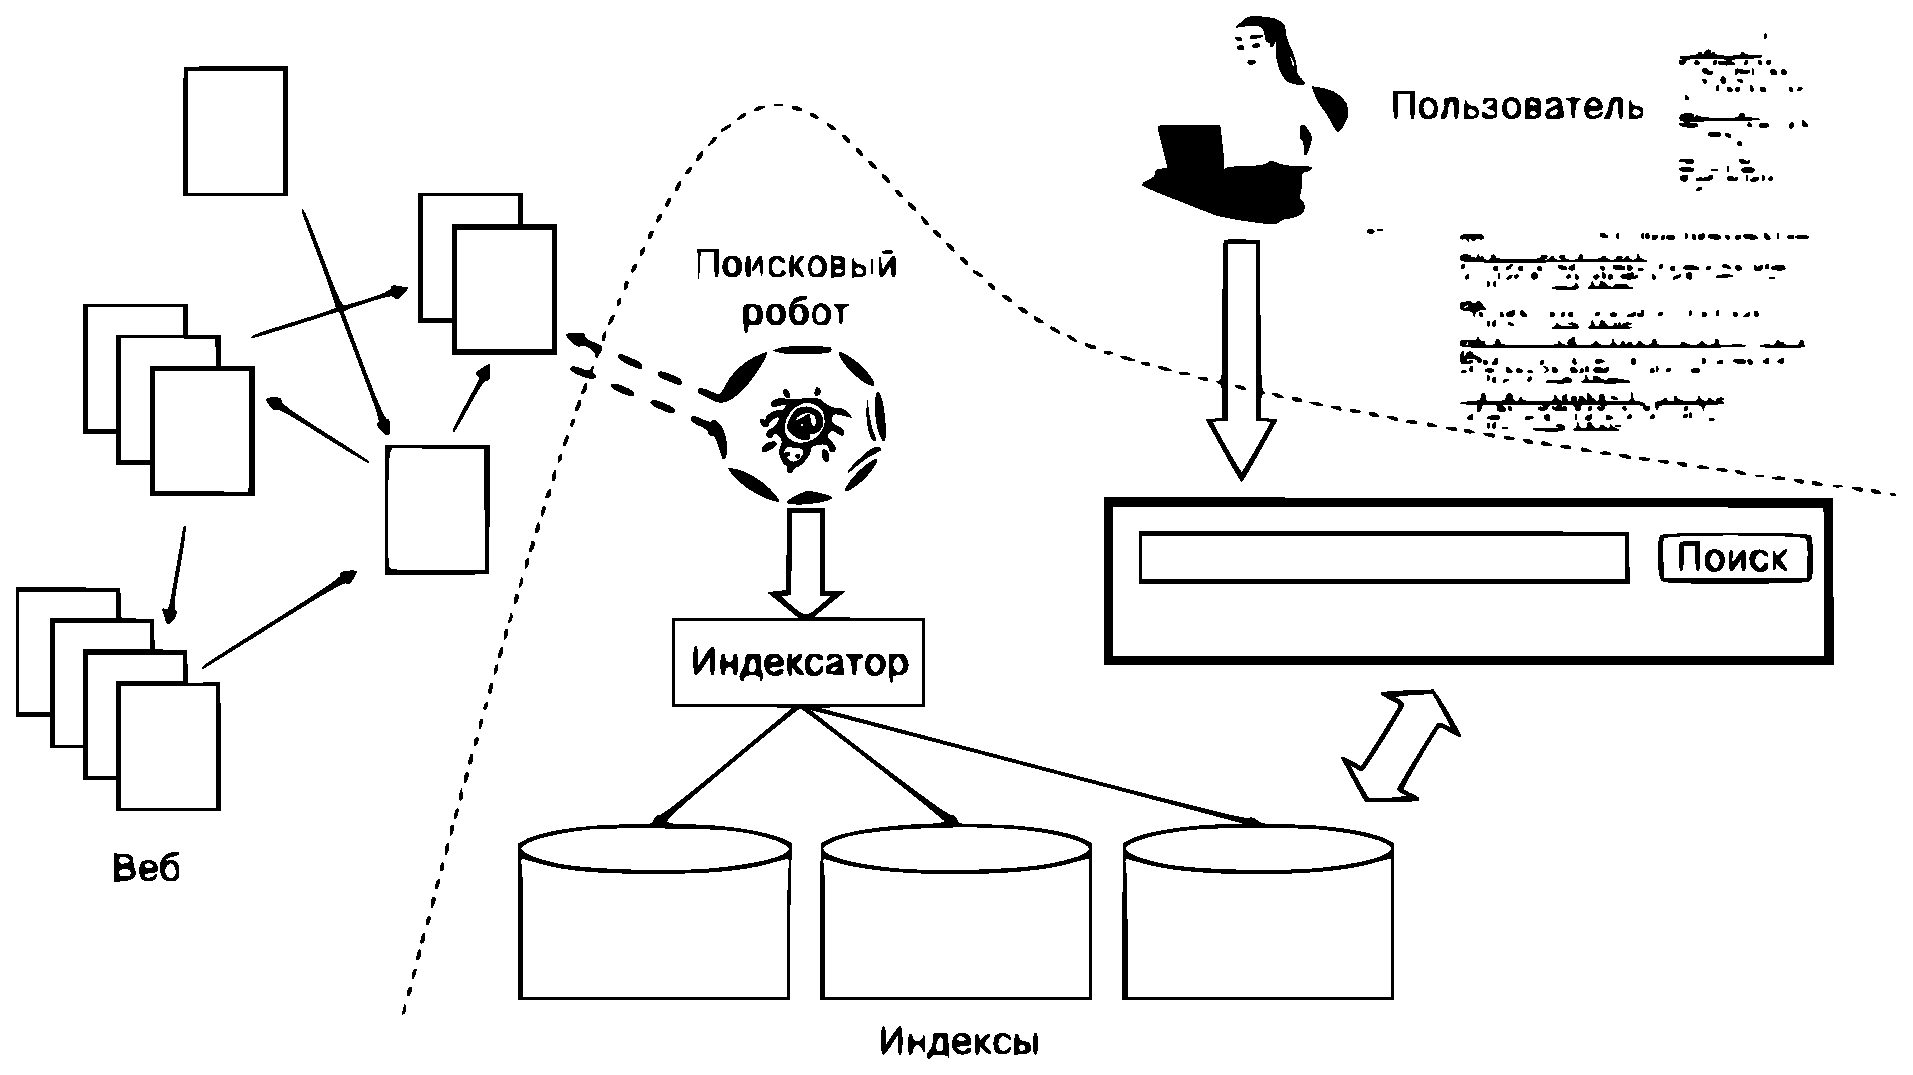
\includegraphics[width=1\linewidth]{irws_comps}}
\caption{Компоненты информационно-поисковой веб-системы}
\label{irws_comps:image}
\end{figure}

\subsection{Обзор поисковой системы Google}
На данный момент поисковая система Google всецело доминирует на мировом рынке ИПВС. Имея главной целью улучшение качества поисковых систем, Google реализовала ряд оригинальных идей в своей ИПВС. Поэтому стоит достаточно подробно рассмотреть высокоуровневую архитектуру её системы, которая изображена на рисунке 1.2. Стоит отметить, что в большая часть системы реализована на языках C и C++ для эффективности работы.

\begin{figure}[H]
\center{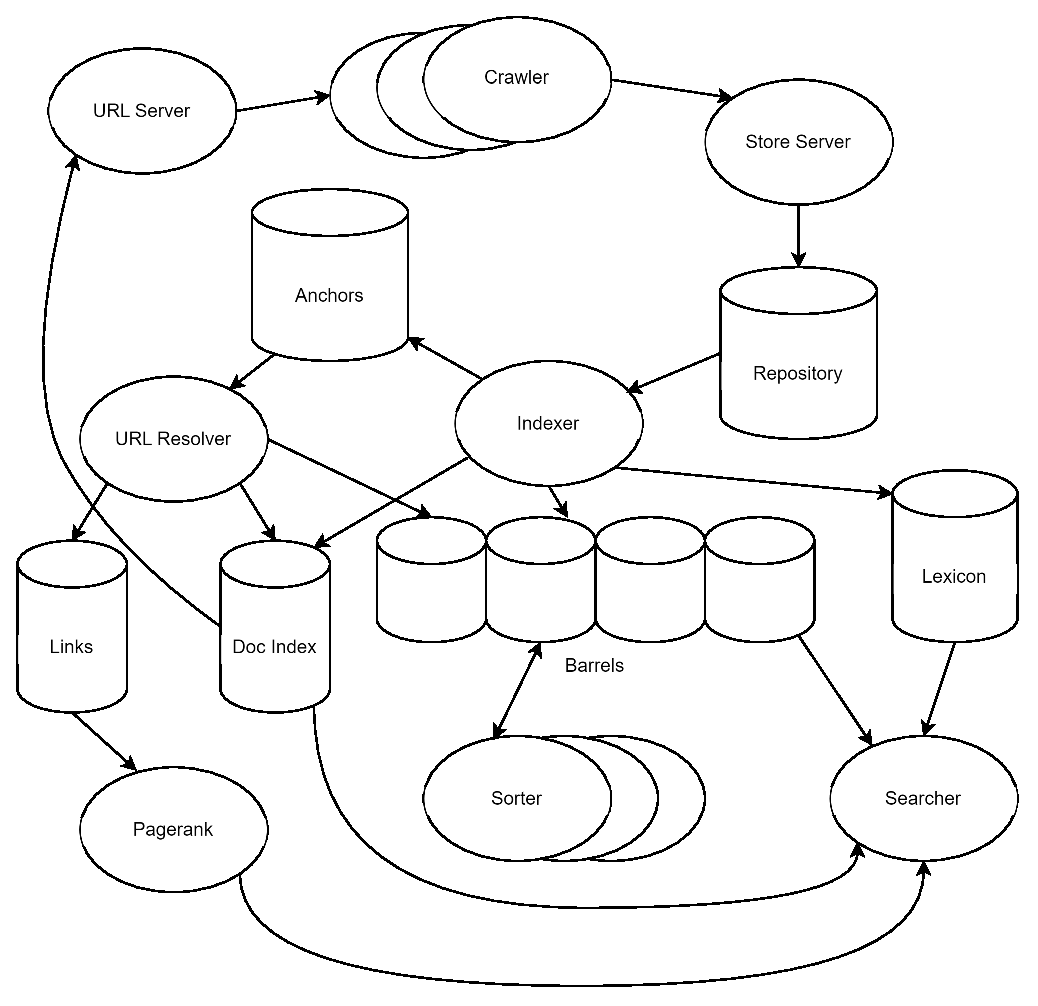
\includegraphics[width=1\linewidth]{google_concept}}
\caption{Высокоуровневая архитектура системы Google}
\label{google_concept:image}
\end{figure}

Веб-сканеры (сrawlers) -- несколько распределенных поисковых роботов, задача которых полностью соответствует определению. Большое количество предъявляемых к ним требований делает их сложным компонентом любой крупномасштабной системы. 
Для масштабирования до сотен миллионов веб-страниц в Google существует система быстрого распределенного сканирования. Один URL-сервер обслуживает списки URL-адресов для нескольких сканеров (обычно около 3). Каждый сканер поддерживает примерно 300 открытых соединений одновременно. Это необходимо для получения веб-страниц в достаточно быстром темпе. На пиковых скоростях система может сканировать более 100 веб-страниц в секунду, используя четыре сканера. Это составляет примерно 600 КБ данных в секунду. Основное снижение производительности — поиск DNS. Каждый сканер поддерживает свой собственный кэш DNS, поэтому ему не нужно выполнять поиск DNS перед сканированием каждого документа. Каждое из сотен соединений может находиться в нескольких различных состояниях:
\begin{itemize}
\item поиск DNS;
\item подключение к хосту;
\item отправка запроса;
\item получение ответа.
\end{itemize}
Поисковые роботы Google используют асинхронный ввод-вывод для управления событиями и ряд очередей для перемещения выборок страниц из состояния в состояние.

Компонент URL-сервер имеет доступ к базе данных URL-адресов страниц и занимается распределением этих адресов между поисковыми роботами.

Страницы, которые обработали поисковые роботы, отправляются в сервис Store, называемый сервером хранилища. Там веб-страницы сжимаются и сохраняются в хранилище (Repository). С каждой веб-страницей связан соответствующий идентификационный номер, называемый docID, который назначается при каждом анализе нового URL-адреса на веб-странице.

Хранилище  (Repository) содержит полный HTML-код каждой веб-страницы. Каждая страница сжимается с помощью zlib, что обусловлено компромиссом между скоростью и степенью сжатия. 
В хранилище документы хранятся один за другим и имеют префикс docID, длину и URL. Для доступа к хранилищу не требуется никаких других структур данных, что помогает обеспечить согласованность данных и значительно упрощает разработку.

Индекс всех документов представлен в "<бочках"> (Barrels), которые хранят два типа индексных структур. В "<передних бочках"> хранится прямой (форвардный, от англ. forward), а в "<задних бочках"> -- инвертированный (перевернутый, от англ. invert) индекс. Рассмотрим эти типы индексов:
\begin{itemize}
\item прямой индекс -- сложная структура данных, по сути являющаяся трехуровневым списком, где первый уровень -- идентификаторы документов (docID), второй -- слова, входящие документ, третий -- позиции вхождения конкретного слова в конкретный документ.
В системе такой индекс уже частично отсортирован по docID и хранится в нескольких (64) "<бочках">. Вместо того, чтобы хранить фактические wordID, каждое wordID сохраняется как относительное отличие от минимального wordID;
\item инвертированный индекс -- структура данных, похожая на прямой индекс, только теперь на первом уровне вложенности списков стоят идентификаторы слов (wordID), а на втором -- идентификаторы документов (docID), за что он и называется "<перевернутым">. В случае, если на третьем уровне вложенности в списках хранятся позиции вхождения слов в документ, такой индекс называют координатным. Преимущество этой структуры данных в том, что по wordID можно быстро найти все документы и позиции вхождения этого слова в них, чем активно пользуется поисковик (Searcher).
Инвертированный индекс генерируется на основе прямого за счет обработки последнего специальным распределенным компонентом -- сортировщиком (Sorter), о котором будет сказано дальше.
\end{itemize}

Функции индексации возлагаются на непосредственно индексатор (Indexer) и сортировщик (Sorter). Индексатор выполняет ряд функций. Он читает хранилище, распаковывает документы и анализирует их. Каждый документ преобразуется в набор вхождений слов, называемых попаданиями (хиты, от англ. hit). Хиты записывают слово, положение в документе, приблизительный размер шрифта и заглавные буквы. Каждое слово преобразуется в wordID с помощью хэш-таблицы в памяти —- лексикона. Новые добавления в хэш-таблицу лексикона записываются в файл. После преобразования слов в wordID их вхождения в текущем документе преобразуются в списки совпадений и записываются в "<передние бочки"> (Barrels). Эта фаза хороша тем, что она может быть эффективно распараллелена между несколькими серверами для увеличения производительности. Также индексатор анализирует все ссылки на каждой веб-странице и сохраняет важную информацию о них в файле привязок (Anchors). Этот файл содержит достаточно информации, чтобы определить, куда указывает каждая ссылка, и текст ссылки. 

Сортировщик (Sorter) берет бочки (Barrels), отсортированные по docID, и сортирует их по wordID для генерации инвертированного индекса. Этот процесс происходит по одной "<бочке"> за раз, поэтому требует небольшого временного хранения. Кроме того, фаза сортировки распараллеливается таким образом, чтобы использовать столько машин, сколько возможно, просто запустив несколько сортировщиков, которые могут обрабатывать разные сегменты одновременно. Поскольку "<бочки"> не помещаются в основную память, сортировщик дополнительно подразделяет их на корзины, которые помещаются в память на основе wordID и docID. Затем сортировщик загружает каждую корзину в память, сортирует ее и записывает в "<задние бочки"> -- в место для хранения инвертированного индекса.

Средство распознавания URL-адресов (URL Resolver) считывает файл привязок (Anchors) и преобразует относительные URL-адреса в абсолютные URL-адреса и, в свою очередь, в docID. Он помещает текст привязки в прямой индекс, связанный с docID, на который указывает привязка. Он также создает базу данных ссылок (Links);

База данных ссылок (Links) представляет собой пары docID. Она используется для вычисления PageRanks для всех документов.

База данных индексов документов (Doc Index) -- упорядоченный по docID индекс последовательного доступа, который хранит информацию о каждом документе. Информация, хранящаяся в каждой записи, включает текущее состояние документа, указатель на хранилище, контрольную сумму документа и различные статистические данные. Если документ был отсканирован, он также содержит указатель на файл переменной ширины с именем docinfo, который содержит его URL и заголовок. В противном случае указатель указывает на список URL, который содержит только URL. Кроме того, есть файл, который используется для преобразования URL-адресов в docID. Это список контрольных сумм URL с соответствующими им docID и отсортирован по контрольной сумме. Чтобы найти docID определенного URL-адреса, вычисляется контрольная сумма URL-адреса и выполняется двоичный поиск в файле контрольных сумм, чтобы найти его docID. URL-адреса могут быть преобразованы в docID в пакетном режиме путем слияния с этим файлом. Это метод, который преобразователь URL-адресов использует для преобразования URL-адресов в docID. Этот пакетный режим обновления имеет решающее значение, потому что в противном случае необходимо выполнять один поиск для каждой ссылки, при условии, что один диск потребует более 32 месяцев для набора данных Google из 322 миллионов ссылок.

На схеме также присутствует база данных доступных слов (Lexicon). В ней хранится информация о проанализированных словах. Как правило, она умещается в оперативную память размером 256 мб. Лексикон реализован как список, каждый элемент которого как минимум имеет свой wordID, само значение слова и список указателей на задние "<бочки"> с инвертированными индексами, в которых содержится wordID.

В Google используется специальная система, которая каждому документу из обойденного веб-графа присваивает число (ранг), как правило нормализованное на отрезке $[0, 1]$, беря в расчет входящие и исходящие ссылки, которая называется PageRank. Прежде чем перейти к её формальному описанию, стоит сначала разобрать интуитивный подход к обосновнию её эффективности на практике. 

Веб-страница может иметь высокий PageRank, если существует много страниц, которые на нее указывают, или если есть несколько страниц, которые указывают на нее и имеют высокий PageRank. Интуитивно понятно, что страницы, которые хорошо цитируются во многих местах в Интернете, заслуживают внимания. Кроме того, страницы, которые имеют, возможно, только одну ссылку от чего-то вроде домашней страницы Yahoo  также вообще стоит посмотреть. Если страница была не высокого качества или была неработающей ссылкой, вполне вероятно, что домашняя страница Yahoo не будет ссылаться на нее. PageRank обрабатывает как эти случаи, так и все, что находится между ними, путем рекурсивного распределения весов через структуру ссылок в Интернете.

Таким образом, число ссылок и обратных ссылок дает некоторое представление о важности или качестве страницы. PageRank расширяет эту идею, не считая ссылки со всех страниц в равной степени, и нормализуя по количеству ссылок на странице. PageRank определяется следующим образом:
Изначально предполагается, что страница $A$ имеет страницы $T_1, T_2, \cdots T_n$, которые ссылаются (цитируют) её. Также существует параметр d, который представляет собой коэффициент демпфирования, который можно установить в диапазоне от 0 до 1, но обычно его принимают за $0.85$. За $C(A)$ принимается количество ссылок, выходящих за пределы страницы $A$. В таком случае PageRank (PR) страницы $A$ определяется следующим образом:

\begin{equation}
PR(A) = (1 - d) + d * \sum_{i = 1}^{n}\frac{PR(T_i)}{C(T_i)}
\end{equation}

Также стоит отметить, что PageRank основан на распределении вероятностей по веб-страницам, поэтому сумма PageRank всех веб-страниц будет равна единице. PageRank может быть вычислен с использованием простого итеративного алгоритма и соответствуют главному собственному вектору нормализованной матрицы ссылок сети. Кроме того, PageRank для 26 миллионов веб-страниц может быть рассчитан за несколько часов на рабочей станции среднего размера. 

Google имеет специальную систему ранжирования. Как было сказано ранее, каждое попадание слова в документ хранит позицию, размер шрифта и наличие заглавных букв. Все эти факторы естественно должны влиять на ранг документа. Поэтому при разработке системы ранжирования было сделано так, чтобы она имела возможность учесть большое множество ранговых характеристик таким образом, чтобы ни одна из них не могла оказаться слишком большого влияния на итоговый ранг страницы.Чтобы ранжировать документ по запросу из одного слова, Google просматривает список совпадений этого слова по этому слову. Google считает, что каждое попадание относится к одному из нескольких различных типов (заголовок, якорь, URL, большой шрифт обычного текста, маленький шрифт обычного текста и т.д.), каждый из которых имеет свой собственный вес шрифта. Веса типов составляют вектор, индексированный по типу. Google подсчитывает количество совпадений каждого типа в списке совпадений. Затем каждый отсчет преобразуется в счетный вес. Веса счетчика сначала увеличиваются линейно с счетом, но быстро сужаются, так что больше определенного счета не поможет. Мы берем скалярное произведение вектора весов типов с вектором весов счетчиков, чтобы вычислить оценку IR (Information Relevance) для документа. Наконец, IR балл объединяется с PageRank, чтобы дать итоговый рейтинг документу.

Для поиска по нескольким словам ситуация более сложная. Теперь несколько списков совпадений должны сканироваться одновременно, чтобы совпадения, встречающиеся близко друг к другу в документе, были взвешены выше, чем совпадения, происходящие далеко друг от друга. Хиты из нескольких списков совпадений сопоставляются друг с другом, поэтому соседние совпадения сопоставляются друг с другом. Для каждого соответствующего набора совпадений вычисляется близость. Близость основана на том, насколько далеко друг от друга находятся совпадения в документе (или привязке), но классифицируется на 10 различных «корзин» значений в диапазоне от совпадения фразы до «даже не близко — not even close». Счет рассчитывается не только для каждого типа попадания, но и для каждого типа и близости. У каждого типа и пары близости есть тип-прокси-вес (type-prox-weights). Счетчики преобразуются в весовые коэффициенты, и мы берем точечное произведение весовых значений счетчиков и весов типа prox для расчета IR-оценки.

Когда дело доходит до непосредственного поиска, то его главная цель -- обеспечить качественные результаты на выходе. В Google процесс поиска состоит из следующих шагов:
\begin{enumerate}
\item Синтаксический разбор запроса.
\item Преобразование слов в идентификаторы слов с помощью лексикона (компонент Lexicon).
\item Поиск начала списка документов для каждого слова в инвертированном индексе.
\item Просмотр списков документов, пока не найдется документ, соответствующий всем условиям поиска.
\item Вычисление рейтинга этого документа для запроса, учитывая IR и PageRank.
\item Если итерация происходит на момент нахождения в коротких бочках и в конце любого списка документов, то производится поиск начала полной бочки для каждого слова из запроса и происходит переход к шагу 4.
\item Если итерация не происходит на момент нахождения  в конце какого-либо списка документов, то происходит переход к шагу 4. 
\item По рангу сортируются документы и выбирается k документов с наибольшим его значением.
\item С помощью базы индексов документов (Doc Index) каждому документу по docID сопоставляется определенный URL-адрес, а также вырезаются отрывки (snippets) в соответствие с запросом.
\item Возвращается ответ на запрос.
\end{enumerate}
\section{Техническое задание}
\subsection{Основание для разработки}

Основанием для разработки является задание на выпускную квалификационную работу бакалавра "<Разработка распределенной поисковой системы для Интернета">.

\subsection{Цель и назначение разработки}

Основной задачей выпускной квалификационной работы является разработка и развертывание распределенной поисковой системы для Интернета.

Функциональное назначение продукта заключается в предоставлении возможности поиска необходимой информации по текстовому запросу в рамках Всемирной паутины конечному пользователю.

Задачами данной разработки являются:
\begin{itemize}
\item разработка глобальной распределенной архитектуры системы;
\item разработка сервиса наполнения исходного множества сайтов для анализа;
\item разработка поискового робота;
\item проектирование базы данных проиндексированных документов;
\item разработка сервиса индексирования документов;
\item разработка сервиса поиска;
\item разработка поискового web-сайта;
\end{itemize}

\subsection{Требования к программной системе}

\subsubsection{Функциональные требования к программной системе}

Выделим следующие общие требования к программной системе:
\begin{itemize}
\item система должна проводить поиск только по доступным из WEB-пространства документам;
\item система должна быть способна выполнять полнотекстовый поиск документов;
\item система должна использовать поисковых роботов для получения целевого множества документов для поиска;
\item система должна быть распределенной и состоять из следующих функциональных компонентов:
\begin{itemize}
\item поисковый робот - компонент, использующийся для получения множества документов из WEB-пространства, по которым будет осуществляться поиск;
\item индексатор - компонент, создающий поисковый индекс по доступным ему документам для эффективного поиска по ним;
\item поисковик - компонент, задача которого по заданному текстовому запросу найти некоторое множество наиболее релевантных документов, используя поисковый индекс;
\item веб-сайт - компонент, с помощью которого конечный пользователь может взаимодействовать с поисковой системой путем ввода запросов и получения списка ресурсов, которые лучше всего соответствуют ожиданиям пользователя по мнению системы;
\item системный журнал - компонент, который отвечает за сбор результатов работы робота, индексатора и поисковика;
\end{itemize}
\end{itemize}

На рисунке 2.1 приведена концептуальная модель программной системы.

\begin{figure}
\center{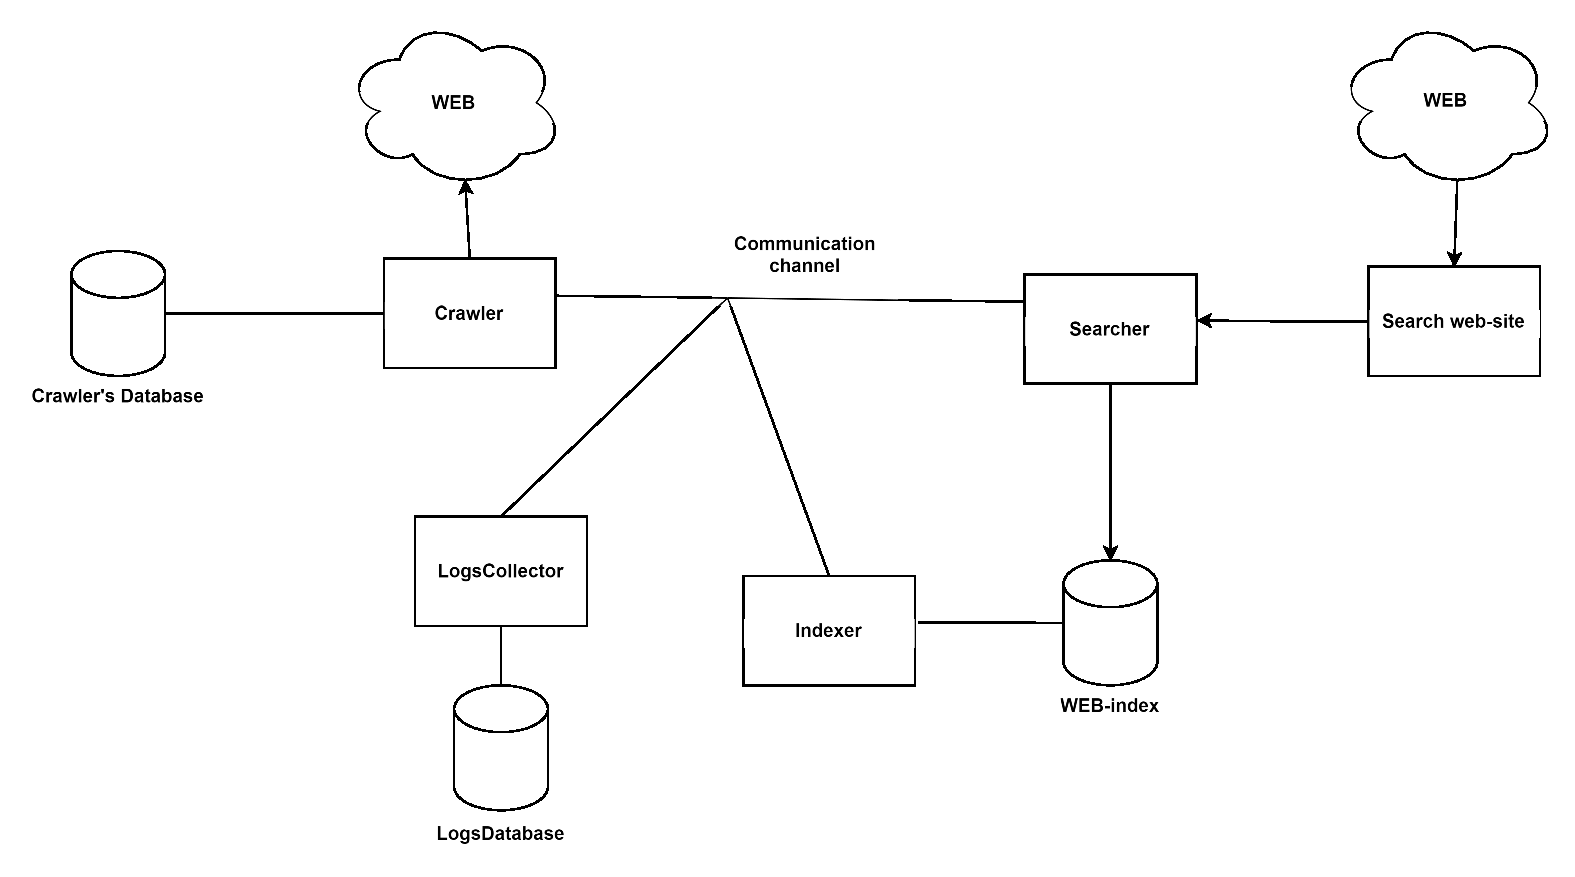
\includegraphics[width=1\linewidth]{concept_system_model}}
\caption{Концептульная модель распределенной поисковой системы}
\label{concept_system_model:image}
\end{figure}

\subsubsection{Функциональные требования к поисковому роботу}
Выделим следующие требования к поисковому роботу:
\begin{itemize}
\item эффективность - поисковый робот должен эффективно использовать разнообразные ресурсы поисковой системы, включая процессор, память и полосу пропускания компьютерной сети;
\item вежливость - робот должен знать и соблюдать явные и неявные правила, регулирующие частоту обращеня поисковых роботов;
\item гибкость - робот должен быть организован таким образом, чтобы иметь возможность обрабатывать разные типы документов;
\end{itemize}

На рисунке 2.2 приведена концептуальная модель поискового робота распределенной поисковой системы.

\begin{figure}
\center{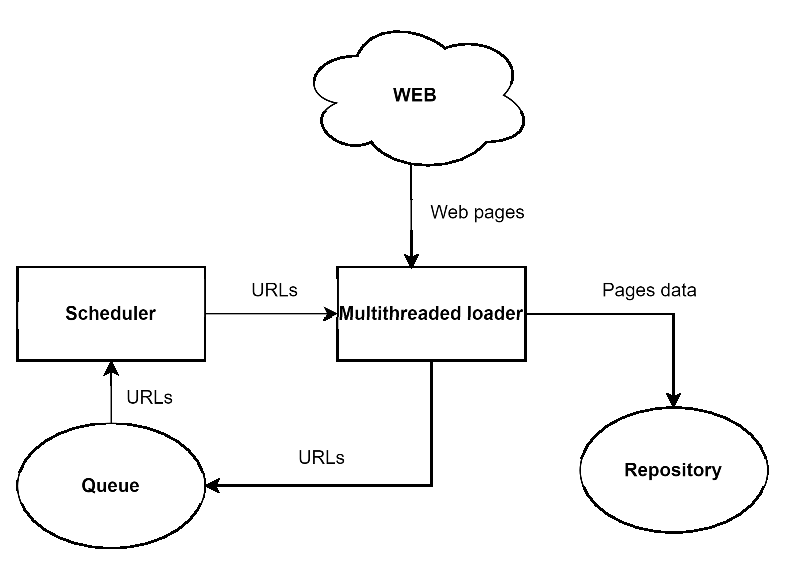
\includegraphics[width=1\linewidth]{robot/concept_robot_model}}
\caption{Концептульная модель поискового робота распределенной поисковой системы}
\label{concept_robot_model:image}
\end{figure}

\subsubsection{Функциональные требования к индексатору}
Выделим следующие требования к индексатору:
\begin{itemize}
\item индексатор должен иметь механизмы взвешенного ранжирования терминов внутри документа;
\item индексатор должен иметь возможность статической оценки документа на основе входящих и исходящих ссылок;
\item индексатор должен быть отказоустойчив независимо от размера потока обрабатываемых документов.
\item индексатор должен эффективным в утилизации ресурсов и производительности.
\end{itemize}

На рисунке 2.3 приведена концептуальная модель индексатора распределенной поисковой системы.

\begin{figure}
\center{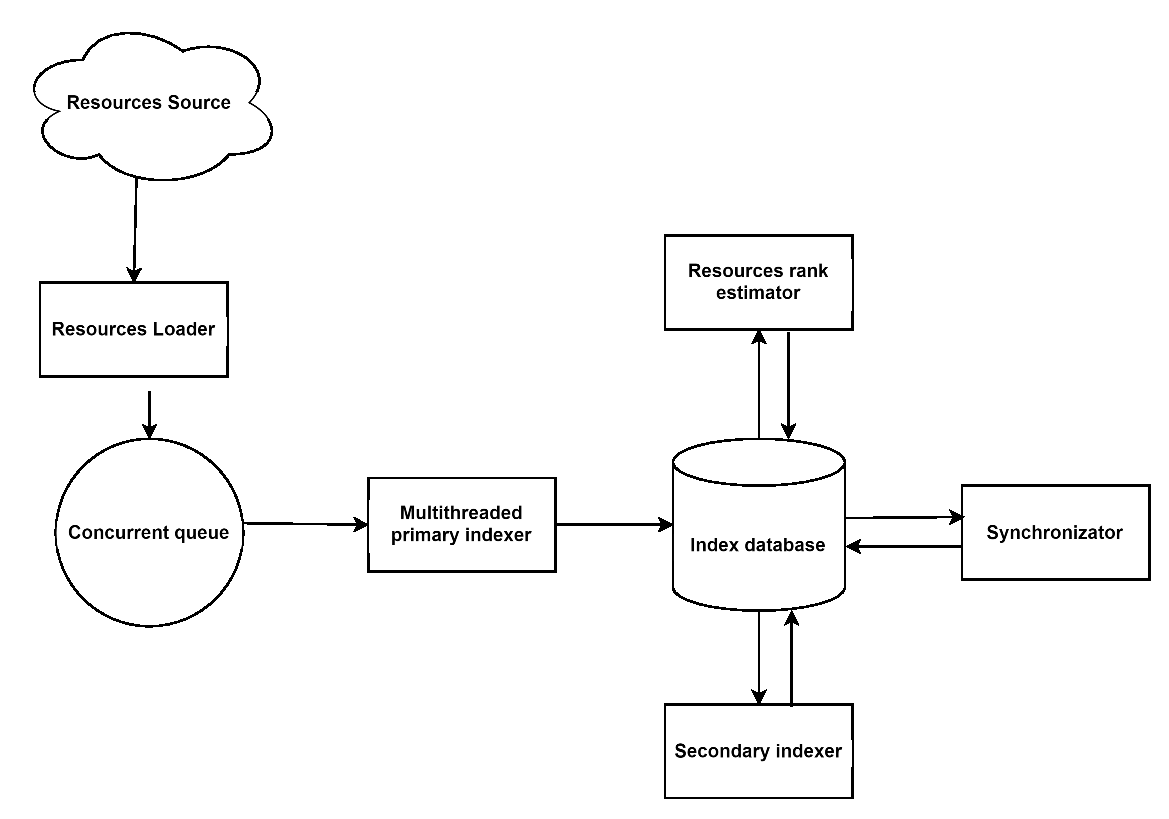
\includegraphics[width=1\linewidth]{indexer/concept_indexer_model}}
\caption{Концептульная модель индексатора распределенной поисковой системы}
\label{concept_indexer_model:image}
\end{figure}

\subsubsection{Функциональные требования к поисковику}
Выделим следующие требования к поисковику:
\begin{itemize}
\item поисковик должен уметь обслуживать одновременно несколько запросов;
\item поисковик должен уметь обрабатывать свободные текстовые запросы;
\item поисковик должен предоставлять публичный API для работы других сервисов;
\item поисковик должен иметь алгоритм подсчета релевантности документов на основе динамических характеристик запроса и статических параметров из индекса;
\item поисковик должен иметь предусмотренные механизмы частичного или полного кеширования результатов пользовательских запросов.
\end{itemize}

На рисунке 2.4 приведена концептуальная модель поисковика распределенной поисковой системы.

\begin{figure}
\center{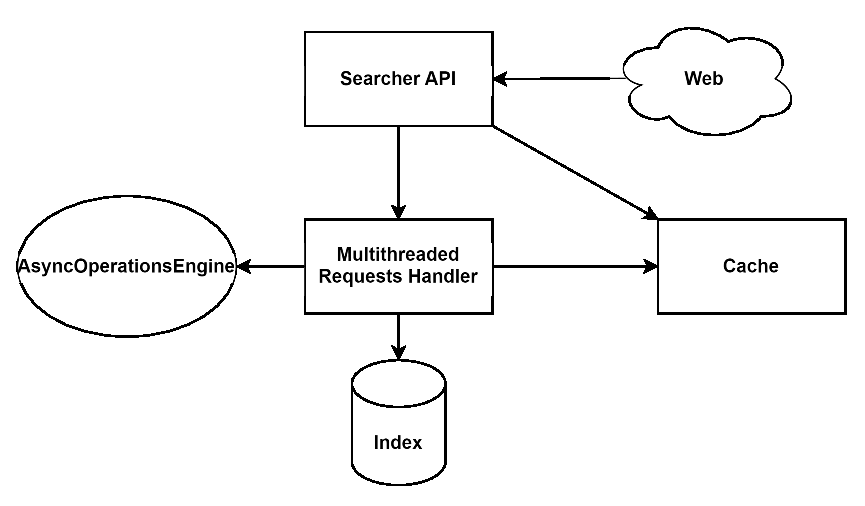
\includegraphics[width=1\linewidth]{searcher/concept_searcher_model}}
\caption{Концептульная модель поисковика распределенной поисковой системы}
\label{concept_searcher_model:image}
\end{figure}

\subsubsection{Моделирование вариантов использования системы}

Для разрабатываемой системы была реализована модель, которая обеспечивает наглядное представление вариантов её использования.

Она помогает в физической разработке и детальном анализе взаимосвязей объектов. При построении диаграммы вариантов использования применяется унифицированный язык визуального моделирования UML.

В системе можно выделить два типа действующих лиц: пользователь и администратор. 

Для пользователя должны быть реализованы следующие прецеденты:
\begin{enumerate}
\item Ввод текстового запроса с последующим получением отражированных результатов поиска.
\item Просмотр наиболее подходящих результатов поиска по запросу с возможностью страничной навигации.
\end{enumerate}

Для администратора должны быть реализованы следующие прецеденты:
\begin{enumerate}
\item Просмотр текущей диагностической информации по работе поискового робота.
\item Просмотр текущей диагностической информации по работе индексатора.
\item Просмотр текущей диагностической информации по работе  поисковых сервисов.
\item Удаленный просмотр логов.
\end{enumerate}

На рисунке 2.5 представлена диаграмма вариантов использования.

\begin{figure}
\center{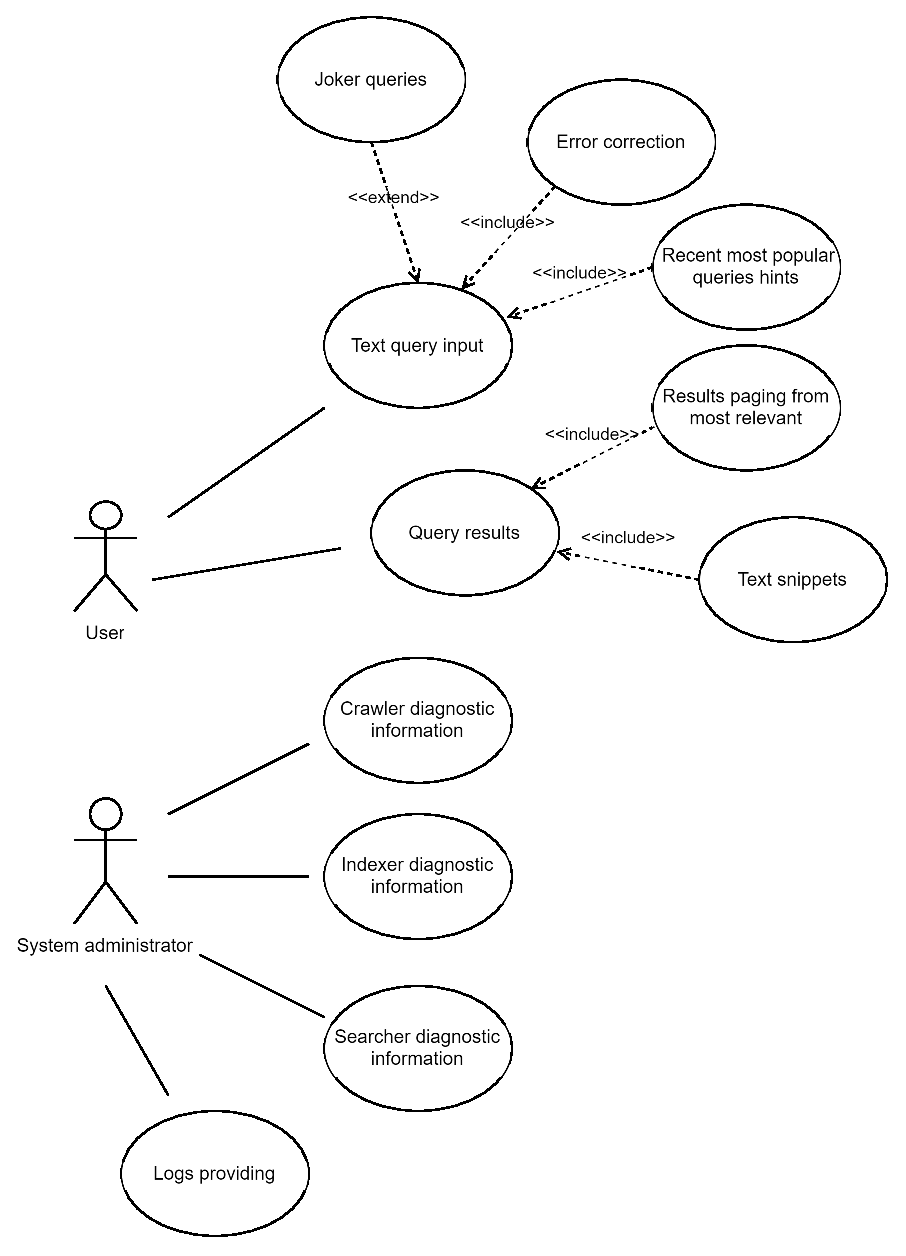
\includegraphics[width=1\linewidth]{diagram_usecases}}
\caption{Диаграмма вариантов использования системы}
\label{diagram_usecases:image}
\end{figure}

\subsubsection{Требования пользователя к интерфейсу web-сайта}

Сайт должен включать в себя:
\begin{itemize}
	\item стартовую страницу поиска с полем для ввода запросов;
	\item страницу с отображенными результатами поиска;
	\item механизм парцеального отображения результатов с возможностью страничной навигации.
\end{itemize}

На рисунках 2.6 - 2.7 представлены макеты веб-сайтов для взаимодействия пользователя с системой.
\begin{figure}
\center{\includegraphics[width=1\linewidth]{site_main}}
\caption{Главная страница поискового веб-сайта}
\label{site_main:image}
\end{figure}
\begin{figure}
\center{\includegraphics[width=1\linewidth]{site_search}}
\caption{Страница отображения результатов поиска}
\label{site_search:image}
\end{figure}

\subsection{Нефункциональные требования к программной системе}

\subsubsection{Требования к архитектуре}

Распределенная система должна иметь микросервисную архитекутуру с целью уменьшить связанность и стать пригодной для горизонтального масштабирования. Взаимодействие компонентов должно осуществляться с использованием брокера сообщений.

\subsubsection{Требования к аппаратному обеспечению}

Для работы сервисов необходимы сервера на операционной системе Linux. Дисковое пространство должно быть не менее 100 Гб, оперативная память  - не менее 10 Гб, процессор должен быть многоядерный с не менее 4 логическими потоками.

\subsection{Требования к оформлению документации}

Разработка программной документации и программного изделия должна производиться согласно ГОСТ 19.102-77 и ГОСТ 34.601-90. Единая система программной документации.

\newsection
\section{Технический проект}

\subsection{Общие сведения о программной системе}
Необходимо спроектировать и разработать распределенную систему для поиска информации по документам из Интернет-пространства.

Системе на вход подается некоторое множество адресов WEB-ресурсов.
Предполагается, что пространство документов связное и что через данное множество ресурсов достижимы все остальные документы целевого графа, чтобы система в перспективе своей работы могла бы целиком обработать пространство документов, которое соответствует начальному множеству.

Ключевыми компонентами системы будут являться:
\begin{itemize}
\item поисковый робот;
\item индексатор;
\item поисковик.
\end{itemize}

Компоненты имеют кардинально разные требования по функциональности и режимам работы, поэтому должны быть спроектированы независимо друг от друга для достижения низкой связанности и возможности горизонтального масштабирования системы.

Целью разработки данной распределенной программной системы является создание инструмента для эффективного ориентирования в таком быстрорастущем сегменте хранения информации как Интернет.

\subsection{Обоснование выбора технологий проектирования}
Используемые для создания программно-информационной системы
языки и технологии отвечают современным практикам разработки, позволяют достичь высокой производительности и отказоустойчивости системы.

\subsubsection{Язык программирования C++}

Язык программирования C++ является мультипарадигменным компилируемым языком со статической типизацией. Его основные преимущества заключаются в высокой производительности, гибкости, тесной связи с аппаратным обеспечением и поддержкой самых разнообразных конструкций из ООП. Эффективность всех компонентов системы будет зависеть от степени задержки выполняемых операций, поэтому С++ можно считать оптимально подходящим под запросы разработки.

\subsubsection{CMake}

CMake - это кроссплатформенная утилита, автоматизирующая процесс создания файлов сборки для таких компилируемых языков, как C++. В частности, в ОС GNU Linux она генерирует Makefile, который, как известно, ответственен за сборку всех имеющихся исходных файлов в один исполняемый. 

\subsubsection{PostgreSQL}

PostgreSQL выбрана в качестве основной базы данных за её мощные возможности и надежность в работе с большими объемами данных, а также поддержку сложных запросов и транзакций. PostgreSQL предлагает удобные функции для разработчиков, такие как поддержка массивов, храненимых процедур и функций, триггеров, что делает её идеальной для комплексных приложений, требующих масштабируемости и гибкости.

\subsubsection{RabbitMQ} 
RabbitMQ, система управления очередями сообщений, реализующая открытый протокол передачи сообщений AMQP, играет ключевую роль в обеспечении асинхронной обработки данных и интеграции различных частей системы. Эффективное использование RabbitMQ позволяет распределить нагрузку, улучшить производительность приложения и обеспечить надежную обработку сообщений. Аппаратное обеспечение должно соответствовать требованиям по пропускной способности и скорости обработки сообщений, что особенно важно при больших объемах данных.

\subsubsection{Библиотека Boost}

Библиотека Boost является сборником большого множества прикладных и востребованных библиотек на языке С++. Как правило, ни одно крупное приложение, где язык C++ является основным в стеке разработки, не обходится без этой библиотеки.
 
\subsubsection{Библиотека LibCDS}

Библиотека LibCDS (concurrent data structures) - достаточно известная в узких кругах библиотека lock-free (без блокировок) структур данных и алгоритмов. Её выбор обусловлен тем, что практически все программные компоненты предполагают многопоточную работу с данными и многие их них буду разделяться между нитями. Традиционные примитивы синхронизации, как правило, очень неэффективны при большом количестве потоков и при частом вызове, поэтому для повышения производительности системных компонентов было принято решение прибегнуть к структурам данных, свободных от блокировок.

\subsubsection{Библиотека IntelTBB}

Библиотека IntelTBB(Threading Building Blocks) - кроссплатформенная библиотека шаблонов C++, разработанная компанией Intel для параллельного программирования. Библиотека содержит алгоритмы и структуры данных, позволяющие программисту избежать многих сложностей, возникающих при использовании традиционных реализаций потоков. В рамках разработки она нужна будет во много ради Flow Graph. Эта часть библиотеки предоставляет такую абстракцию, как вычислительный граф, где на узлах происходит обработка, а через ребра передаются данные. Можно считать, что она является реализацией паттерна проектирования "<Цепочка обязанностей">, но при этом каждый её элемент по умолчанию имеет возможность для конкурентного исполнения под управлением глобального планировщика потоков. Такой подход будет полезен при проектировании и разработке индексатора.

\subsubsection{Библиотека Libpqxx}

Библиотека Libqpxx - библиотека на C++, написанная поверх библиотеки на языке C libpq, предоставляющая удобные ООП-абстракции для синхронной работы с базой данных PostgreSQL.

\subsubsection{Библиотека AMQP-CPP}

Библиотека AMQP-CPP - библиотека на C++, написанная поверх библиотеки на языке C libamqp, предоставляющая удобные ООП-абстракции для асинхронной работы с брокером сообщений RabbitMQ.

\subsubsection{Библиотека Yaml-Cpp}

Библиотека Yaml-Cpp - библиотека на C++, реализующая синтаксический анализ документов в формате YAML и предоставляющая удобный интерфейс для их чтения и записи. Так как все компоненты системы будут иметь конфигурационные файлы в формате YAML, она бесспорно будет очень полезна.

\subsubsection{Библиотека Cld3}

Библиотека Cld3 - библиотека, созданная и выложенная в открытый доступ компанией Google, предоставляющая обученную нейронную сеть для идентификации языка поданного на вход текстового фрагмента. Она будет полезна в рамках анализа текстовых запросов от пользователей в поисковике.

\subsubsection{Библиотека Libarchive}

Библиотека Libarchive - библиотека, написанная на языке С, предоставляющая средства чтения и записи данных в разных форматах сжатия и архивации.

\subsubsection{Библиотека Gumbo}

Библиотека Gumbo - библиотека на языке C, созданная и выложенная в открытый доступ компанией Google, предоставляющая готовый синтаксический анализатор HTML-документов. Так как наша система ориентирована для анализа документов из Интернета, то анализ HTML-документов должен быть одной из важных задач. 

\subsubsection{Библиотека Libstemmer}

Библиотека Libstemmer - библиотека на языке C, предоставляющая возможность производить операцию стемминга над словами с разделением по языкам, где стемминг - процесс нахождения основы слова для заданного исходного слова. Это будет необходимо для нахождения разделения всего абстрактного множества слов на классы эквивалентности, чтобы тем самым увеличить эффективность поиска. 

\subsubsection{Библиотека RobotsTxt}

Библиотека RobotsTxt - библиотека на языке C++, созданная и выложенная в открытый доступ компанией Google, предоставляющая готовый синтаксический анализатор документов, соответствующих стандарту REP (Robots Exclusion Protocol) - соглашения, которое разрешает владельцам Интернет-ресурсов определять ограничения для посещения страниц поисковыми роботами. Чтобы робот из нашей системы мог считаться "<вежливым">, необходимо иметь поддержку этого протокола в системе.

\subsubsection{Библиотека Quill}
Библиотека Quill - библиотека на языке C++, которая предоставляет средства для высокопроизводительного и гибкого создания журналируемых сообщений, последующий анализ которых позволит делать выводы о качествах работы тех или иных компонентов, что поможет в более прозрачном виде отслеживать ошибки и сбои.

\subsubsection{Библиотека Drogon}
Библиотека Drogon - кроссплатформенная библиотека на языке C++ для создания WEB-приложений. Она предоставляет множество ООП-абстракций, предоставляет полную поддержку асинхронных операций и имеет высокую производительность. Она будет нужна при создании поисковика.

\subsection{Архитектура распределенной системы}

Распределенная система будет представлена набором сервисов с независимыми моделями данных, которые будут взаимодействовать друг с другом посредством брокера сообщений. Подобную структуру можно отнести к классу микросервисных архитектур.

Система будет представлена следующими сервисами:
\begin{itemize}
\item поисковый робот;
\item индексатор;
\item поисковик;
\item сборщик журналируемой информации, поступающей от вышеперечисленных сервисов.
\end{itemize}

Роль брокера сообщений будет исполнять RabbitMQ.

На рисунке 3.1 представлена диаграмма развертывания распределенной поисковой системы.

\begin{figure}
\center{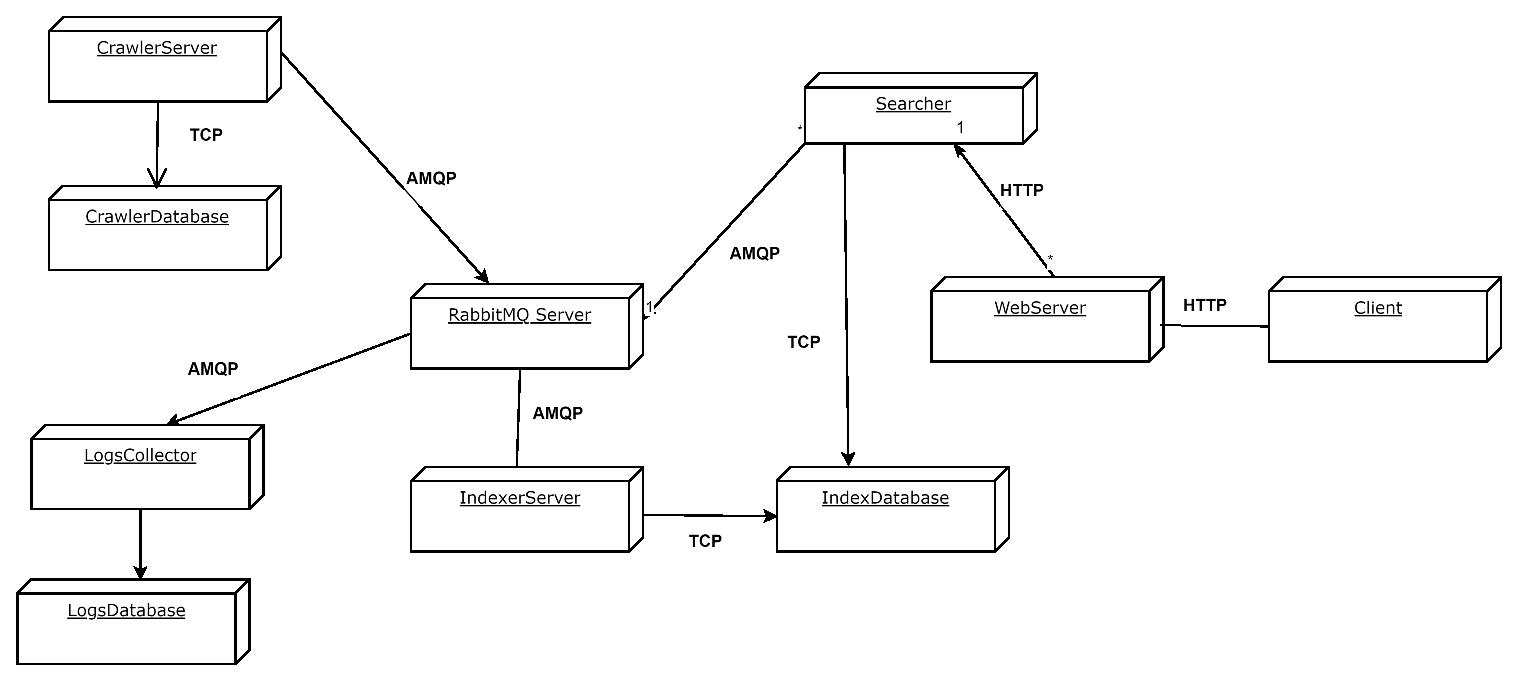
\includegraphics[width=1\linewidth]{diagram_deployment}}
\caption{Диаграмма развертывания распределенной поисковой системы}
\label{diagram_deployment:image}
\end{figure}

\subsection{Поисковый робот}

Поисковый робот предназначен для обхода в ширину веб-графа, которым представлен Интернет. Он сохраняет метаинформацию о документах в базе данных до следующего обхода и переходит по их ссылкам с целью нахождения новых документов на заданном пространстве. После успешной валидация документ отправляется на шину данных для дальнейшей обработки другими компонентами, в частности, индексатором. 

\subsubsection{Типы обрабатываемых документов}
Робот при работе с ресурсами Интернета будет иметь дело со следующими типами документов:
\begin{itemize}
\item файл robots.txt, содержимое которое соответствует протоколу REP, не индексируется;
\item файлы навигации по веб-ресурсу в формате XML, содержимое которых соответствует протоколу SITEMAP, могут быть вложенными, не индексируются;
\item рядовые HTML-документы, которые должны быть проиндексированы системой и порождаются либо корневой страницей веб-ресурса, либо файлами навигации SITEMAP.
\end{itemize}

\subsubsection{Компоненты поискового робота}

На рисунке 3.2 представлена диаграмма компонентов поискового робота.

\begin{figure}
\center{\includegraphics[width=1\linewidth]{robot/diagram_components}}
\caption{Диаграмма компонентов поискового робота распределенной системы}
\label{robot/diagram_components:image}
\end{figure}

\subsubsection{Описание базы данных}

На рисунке 3.3 представлена ER-диаграмма базы данных поискового робота.

\begin{figure}
\center{\includegraphics[width=1\linewidth]{robot/robot_db}}
\caption{ER-диаграмма базы данных поискового робота распределенной системы}
\label{robot/robot_db:image}
\end{figure}

\subsubsection{Описание потоков данных}

На рисунке 3.4 представлена диаграмма потоков данных для поискового робота распределенной системы.

\begin{figure}
\center{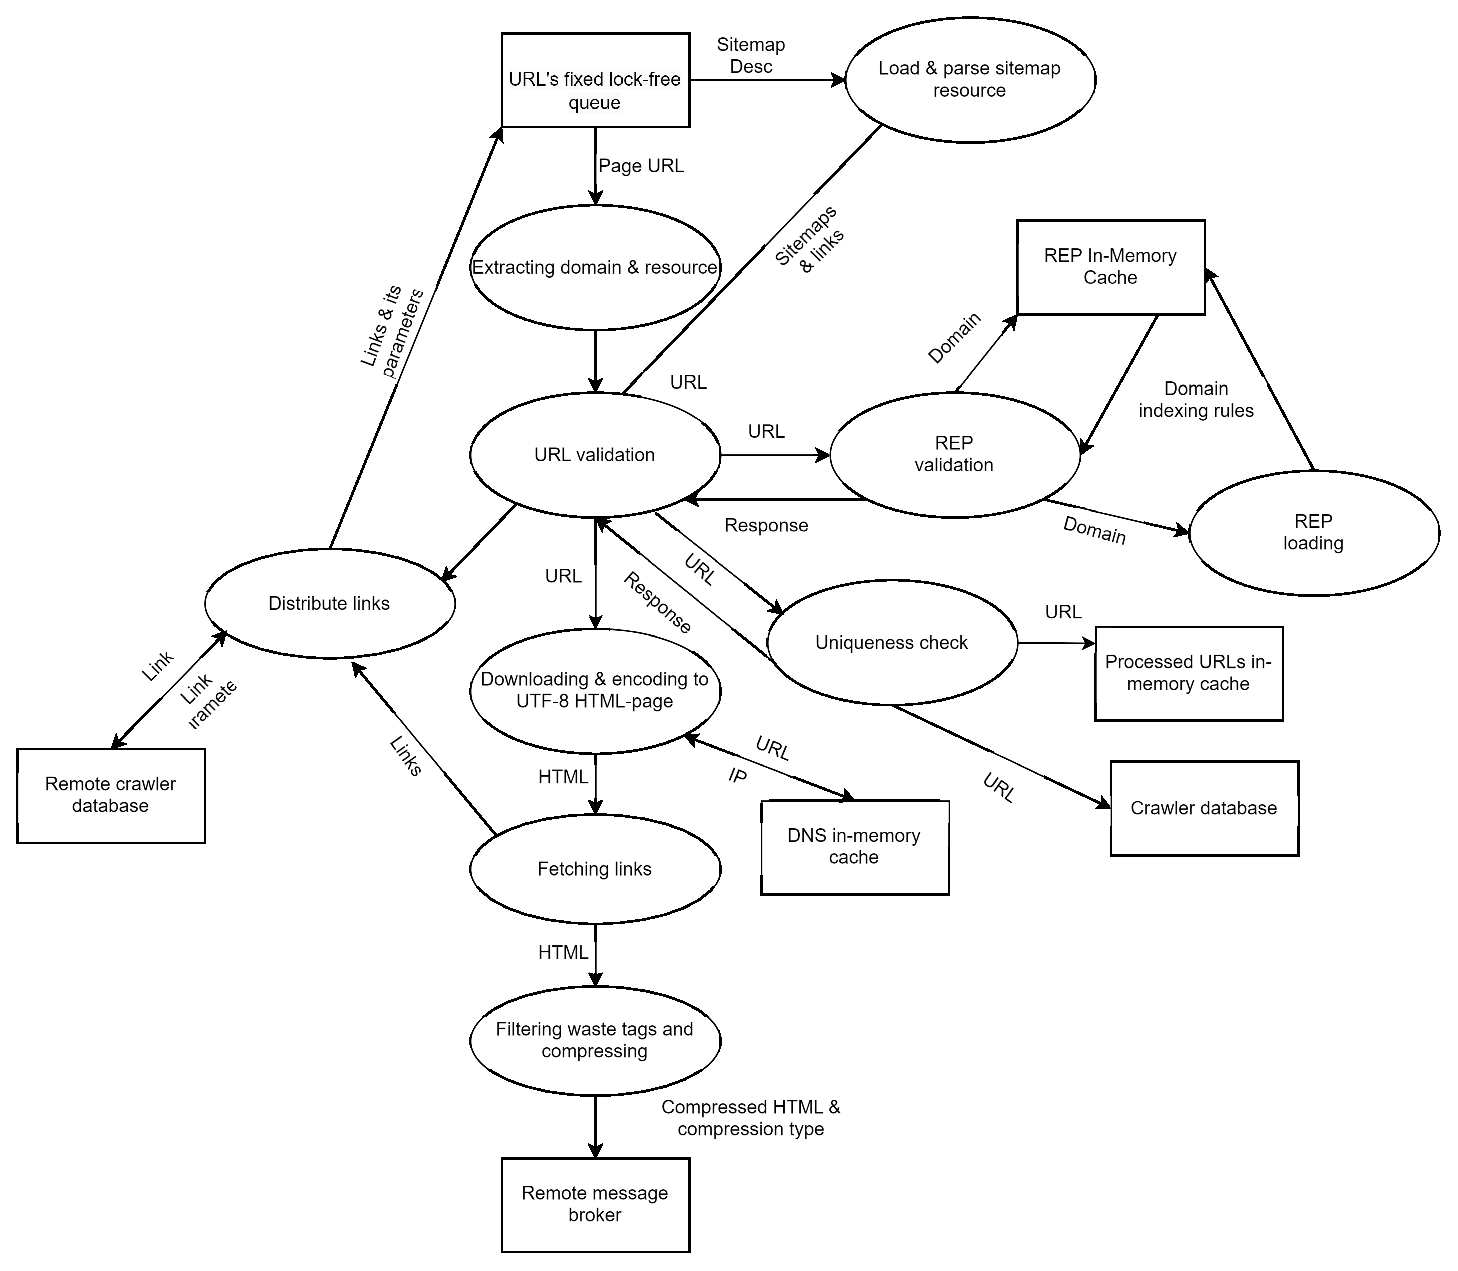
\includegraphics[width=1\linewidth]{robot/diagram_dataflow}}
\caption{Диаграмма потоков данных для поискового робота распределенной системы}
\label{robot/diagram_dataflow:image}
\end{figure}

\subsubsection{Описание концептуальных классов}

На рисунке 3.5 представлена диаграмма концептуальных классов для поискового робота распределенной системы.

\begin{figure}
\center{\includegraphics[width=1\linewidth]{robot/diagram_classes}}
\caption{Диаграмма концептуальных классов для поискового робота распределенной системы}
\label{robot/diagram_classes:image}
\end{figure}

\subsection{Индексатор}

Индексатор - компонент системы, ответственный за статический анализ полученных им документов, результаты которого впоследствии будут использоваться в режиме чтения поисковиком. 
При проектировании и разработке индексатора сосредоточимся на следующих главных задачах:
\begin{itemize}
\item обеспечение контроля сбора ресурсов из брокера сообщений;
\item разработка алгоритма индексирования документов;
\item разработка алгоритма вычисления статического ранга документов.
\end{itemize}

\subsubsection{Описание контроля сбора ресурсов}
Контроль сбора ресурсов будет включать в себя следующие обязательные аспекты:
\begin{itemize}
\item ограничение количества ресурсов для индексирования. После предварительной обработки некоторого натурального числа документов сбор новых прекращается и начинаются следующие стадии индексации;
\item парциальный сбор ресурсов. Ввиду того, что предварительная индексация ресурса выполняется намного дольше, чем его получение из очереди сообщений, разумно делать это парциально, чтобы в конечном итоге не перегрузить оперативную память. По этой причине индексатору будет задаваться размер порции ресурсов для обработки и желаемая скорость в единицах в секунду;
\end{itemize}

\subsubsection{Индексирование документов}

Логической моделью проиндексированных документов будет являться инвертированный индекс. 

Инвертированный индекс - индекс, который представляет собой хеш-таблицу следующей конфигурации: 
\begin{itemize}
\item ключом является термин, как правило, его глобальный целочисленный индентификатор;
\item значение же представляется в виде списка глобальных идентификаторов документов, в которых данный термин был встречен хотя бы один раз.
\end{itemize}

Однако одной лишь структуры мало. Терминов в одном документе может быть много, поэтому необходимо для каждого из них рассчитать их относительный ранг, находящийся в диапазоне от 0 до 1 включительно. Этот ранг будет вычисляться на основе абсолютной взвешенной частоты термина и его обратной документной частоты.

Кроме того, в целях повышения производительности системы организуем индекс так, чтобы поиск по нему мог осуществляться нечетко, но с минимальными потерями в точности и полноте поиска. Этого можно достичь с использованием так называемых "<чемпионских списков">.

Чемпионские списки представляют из себя хеш-таблицу, где ключом выступает целочисленный идентификатор термина, а значением - ограниченный в размере список идентификаторов документов, расположенных по убыванию, начиная с документа, в котором заданный термин имеет максимальный относительный ранг. 

\paragraph{Абсолютная взвешенная частота термина}

Абсолютная взвешенная частота функционально зависит от количество вхождений термина в документ. Но так как мы зачастую будем иметь дело с форматами данных древовидной структуры, таких как HTML, мы можем дополнительно присваивать каждому типу узла свой вес $w$. Кроме того, чтобы учитывать вложенность узлов, необходимо ввести агрегирующую весовую функцию $Agg$. Итак, полная формула вычисления абсолютной взвешенной частоты термина в документе принимает следующий вид:

\begin{center}
$WTF(t) = \sum_{i = 1}^{n}Agg(w_1, w_2, ..., w_m)$
\end{center} где $n$ -- количество вхождений термина данных, а $m$ -- количество взвешенных предков-узлов элемента, в содержание текста которого входит термин $t$.

Смысл абсолютной взвешенной частоты термина достаточно прост. Чем чаще термин встречается в документе, тем выше его последующий ранг. Однако нередки случаи, когда высокая внутридокументная частота термина обусловлена лишь тем, что этот термин входит в число частоиспользуемых. Чтобы снизить влияние данного фактора, вводится понятие обратной документной частоты термина.

\paragraph{Обратная документная частота термина}

Документная частота термина ($DTF$) - количество документов, в которых термин был встречен хотя бы один раз. Обратная документная частота же определяется следующим образом:

\begin{center}
$IDTF(t) = \log\frac{N}{DTF(t)}$
\end{center} где $N$ -- общее количество документов, $DTF(t)$ -- документная частота термина $t$.

Смысл обратной документной частоты заключается в том, что в случае, если термин встречается в большом количестве документов, то независимо от $WTF$ ранг термина будет снижен.

\paragraph{Относительный ранг термина в документе}

Абсолютный ранг термина в документе вычисляется следующим образом:
\begin{center}
$ATR(t) = WTF(t) * IDTF(t)$
\end{center}

В свою очередь, относительный ранг термина вычисляется путем нормализации её абсолютных вариаций:
\begin{center}
$RTR(t) = \frac{ATR(t)}{\sqrt(\sum{i = 1}^{n}ATR(t_1)^2 + ATR(t_2)^2 + ... + ATR(t_m)^2)}$
\end{center} где $m$ -- количество различных терминов в документе.

\subsubsection{Статическое ранжирование документов}

С целью повышения релевантности поисковой выдачи необходимо учитывать конфигурацию веб-графа документов в целом. Поэтому разумно каждому документы присвоить некоторый относительный ранг, который будет зависеть от количества и качества входящих и исходящих ссылок. Интуитивно очевидно, что ранг документа должен быть выше, если выше вероятность перехода на него по гиперссылке. В таком случае мы можем представить документы, как состояния марковской цепи. 

Марковская цепь -- это дискретный стохастический процесс, представляющий собой последовательность временных шагов, на каждом из которых происходит случайн выбор независимо от предыдущего.

Марковская цепь характеризуется матрицей вероятностей переходов $P$, имеющей размерность $N$ x $N$, где $N$ - количество состояний цепи. Сумма элементов в строке матрицы переходов должна равняться 1. В таком случае $P(i, j)$ - вероятность перехода с $i$-ой страницы на $j$-ую.

Матрица с неотрицательными элементами называется стохастической. Ключевое её свойство заключается в том, что она имеет главный левый собственный вектор, соответствующий максимальному значению, которое равно единице.

Также введем определение эргодической марковской цепи.

Марковская цепь называется эргодической, если существует положительное целове число $T_0$, такое. что для всех пар состояний $i$, $j$ в марковской цепи, стартующей в момент $t = 0$ из состояния $i$, для всех $t > T_0$ вероятность нахождения в момент времени $t$ в состоянии $j$ больше нуля.

Иными словами для эргодической марковской цепи должны быть выполнены следующие условия:
\begin{itemize}
\item неразложимость -- гарантирует, что существует последовательность переходов с ненулевой вероятностью из любого состояния в любое другое;
\item апериодичность -- гарантирует, что состояния не делятся на такие множества, что все переходы осуществляются циклически из состояний одного множества в состояния другого множества;
\end{itemize}

И, наконец, для любой эргодической цепи верно следующее утверждение.

Для любой эргодической цепи Маркова существует единственный вектор стационарного распределения вероятностей $\vec{p}$, являющийся главным левым собственным вектором матрицы $P$, и если $f(i, t)$ -- количество переходов в состоянии $i$ за $t$ шагов, то 

\begin{center}
$lim_{t \to \inf}\frac{f(i, t)}{t}=p(i)$
\end{center} где $p(i) > 0$ -- стационарная вероятность состояния $i$.

Чтобы воспользоваться вышеописанное теоретической выкладкой, сформируем модель обхода документов.

Пусть есть некоторый абстрактный "<путешественник">, который в случайном порядке переходит со страницы на страницу.
Определим два несовместных типа переходов:
\begin{itemize}
\item стационарный переход с одной страницы на другую по гиперссылке, который имеет свою вероятностную оценку;
\item телепортация с постоянной вероятностью $\alpha$ c одной страницы на другую не задействуя гиперссылки. Такая возможность сделает нашу марковскую цепь эргодической.
\end{itemize}

Итак, формула полной вероятности перехода с $i$-ой страницы на $j$-ую будет иметь вид:

\begin{center}
$P(i, j) = \frac{1}{L_i} * (1 - \alpha) + \frac{1}{N} * \alpha$
\end{center} где $L_i$ -- количество ненулевых элементов матрицы смежности веб-графа на строке $i$, $N$ -- общее количество документов.

На основе этой формулы мы формируем матрицу в ероятностных переходов марковской эргодической цепи и итеративно приближенно вычисляем её левый собственный вектор, который будет являться стационарным распределением вероятностей между всеми документами из множества, что мы и будем называть статическим рангом документа.

\subsubsection{Компоненты индексатора}

На рисунке 3.6 представлена диаграмма компонентов индексатора.

\begin{figure}
\center{\includegraphics[width=1\linewidth]{indexer/diagram_components}}
\caption{Диаграмма компонентов индексатора распределенной поисковой системы}
\label{indexer/diagram_components:image}
\end{figure}

\subsubsection{Описание базы данных}

Модель данных будет состоять из двух логических частей, физически расположенных в одной базе:
\begin{enumerate}
\item Эталонная часть модели, предназначенная исключительно для чтения поисковиком при обработке пользовательских запросов;
\item Черновая часть модели, предназначенная для создания новых версий индекса, не вмешиваясь во внутреннюю структуру эталонной модели. Она содержит в себе полную копию структуры эталонной модели с несколькими дополнениями, необходимыми для эффективного создания индекса. После завершения создания черновой модели она атомарно целиком заменяет эталонную, при этом полностью очищаясь для создания следующего экземпляра индекса.
\end{enumerate}

На рисунках 3.7 - 3.8 представлены ER-диаграммы эталонной и черновой части базы данных индекса распределенной системы.

\begin{figure}
\center{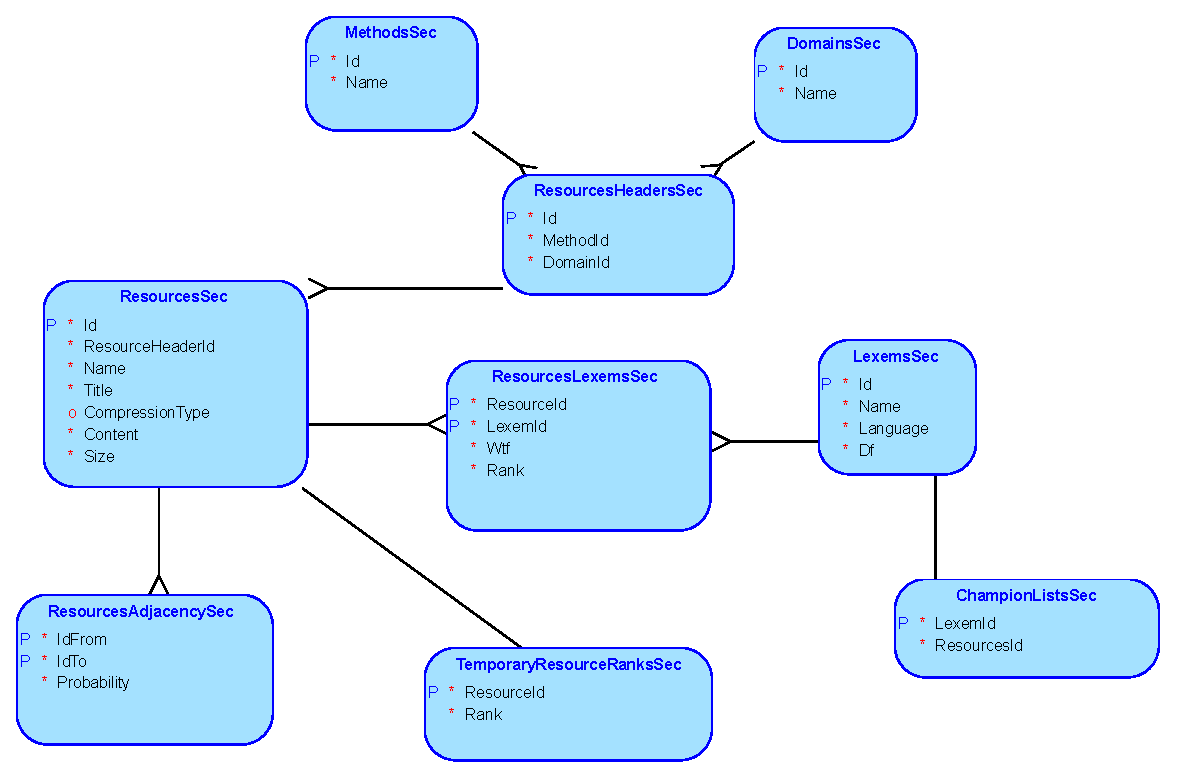
\includegraphics[width=1\linewidth]{indexer/indexer_sec_db}}
\caption{ER-диаграмма черновой части базы данных индексатора распределенной системы}
\label{indexer/indexer_sec_db:image}
\end{figure}

\begin{figure}
\center{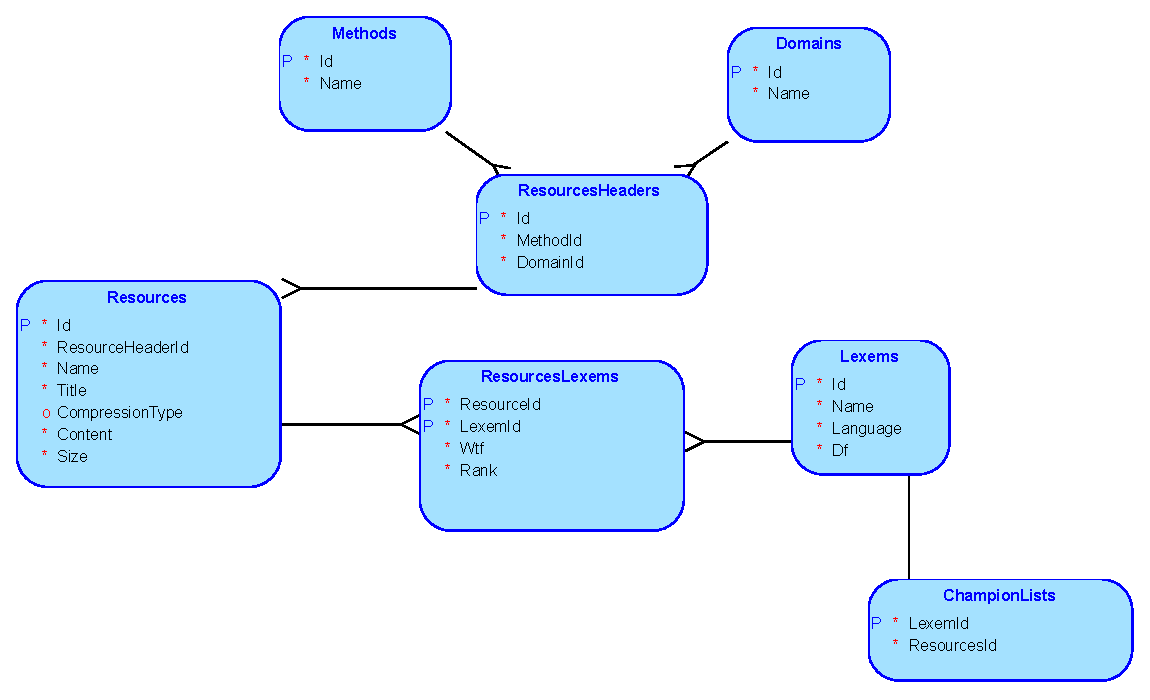
\includegraphics[width=1\linewidth]{indexer/indexer_db}}
\caption{ER-диаграмма эталонной части базы данных индексатора распределенной системы}
\label{indexer/indexer_db:image}
\end{figure}

\subsubsection{Описание концептуальных классов}

На рисунке 3.9 представлена диаграмма концептуальных классов для индексатора распределенной системы.

\begin{figure}
\center{\includegraphics[width=1\linewidth]{indexer/diagram_classes}}
\caption{Диаграмма концептуальных классов для индексатора распределенной системы}
\label{indexer/diagram_classes:image}
\end{figure}

\subsection{Поисковик}

Поисковик предназначен для обработки пользовательских запросов и выдачи релеватных результатов поиска с помощью ранее созданного индекса документов.

\subsubsection{Описание процесса ранжирования документов}

Начнем с того, что заметим, что количество всех веб-документов хоть и велико, но ограничено некоторым натуральным числом. По этой причине количество возможных терминов также ограничено некоторым натуральным числом $T$. 

Следовательно, множество всех веб-документов можно рассмотреть, как конечное векторное пространство размерности $T$. 

В свою очередь, каждый документ определяется некоторым вектором
\begin{center}
$\vec{D}=(r_1, r_2, ..., r_T)$
\end{center} где $r_i$ -- относительный ранг термина с номером $i$ в документе $D$.

Мерой соответствия одного документа другому можно считать косинус угла между их векторами в вышеопределенном векторном пространстве, а именно следующее:

\begin{center}
$R(d_1, d_2)=\frac{\vec{d_1} * \vec{d_2}}{|\vec{d_1}| |\vec{d_2}|}$
\end{center} где $R$ -- мера соответствия документа $d_1$ документу $d_2$ и наоборот.

Пользовательский запрос будет рассматриваться системой как документ, так как фактически тоже имеет своё текстовое значение и определенную смысловую нагрузку. Поэтому для получения меры соответствия запроса какому-либо документу, будет необходимо получить вектор запроса и найти значение косинуса угла между ним и вектором целевого документа.

\subsubsection{Описание алгоритма работы поисковика}
Алгоритм работы поисковика состоит в следующем:
\begin{enumerate}
\item Анализ и разбиение возможного мультиязычного пользовательского запроса на множество отрывков с одинаковым языком. В зависимости от вероятности соответствия предсказанного языка к отрывку присвоить каждому из них свой первоначальный ранг. Добиться подобного функционала можно с использованием нейросетей.
\item С помощью парсера свободных текстовых запросов разбить отрывки на множество лексем в соответствие с правилами. В рамках данной работы предполагаются следующие действия:
\begin{itemize}
\item фильтрация стоп-слов (часто употребимых слов для каждого языка, которые не несут существенной смысловой нагрузки);
\item операция стемминга для присвоения каждой лексемы к конкретному классу эквивалентности.
\end{itemize}
\item Объединить множества лексем из всех отрывков в один большой поток токенов. Пользовательский запрос будет рассматриваться как документ, поэтому каждый токен будет иметь свою взвешенную частотную характеристику, название языка и непосредственно значение. Так как документ всего один - запрос, то в этом случае взвешенная частотная характеристика совпадает с абсолютным рангом токена. По этой причине остается провести лишь операцию нормализации рангов, с целью для каждого термина получить относительный ранг.
\item Получив векторное представление пользовательского запроса, для каждого его термина найдем чемпионские списки и объединим их, получив в конечном итоге целевое множество документов для поиска.
\item Для каждого документа находится косинусная мера его соответствия пользовательскому запросу. По итогу для каждого документа мы имеем $\vec{R}$, у которого есть две составляющие: косинусная мера соответствия запросу (динамическая) и ранг (статическая).
\item С помощью заданного коэффициента приоритета статического критерия над динамическим объединяем две составляющие через нахождение длины $\vec{R}$, будем считать это релевантностью документа.
\item Сортируем документы по убыванию релевантности и отправляем заголовок, URL и релевантность документа в соответствие с заданными параметрами смещения и количества.
\end{enumerate}

\subsubsection{Компоненты поисковика}

На рисунке 3.10 представлена диаграмма компонентов поисковика.

\begin{figure}
\center{\includegraphics[width=1\linewidth]{searcher/diagram_components}}
\caption{Диаграмма компонентов поисковика распределенной поисковой системы}
\label{searcher/diagram_components:image}
\end{figure}
\ifПрактика{}\else{
   \section{Рабочий проект}

\subsection{Спецификация компонентов и классов программной системы}


\subsubsection{Спецификация поискового робота}

Поисковый робот имеет собственный конфигурационный файл "<crawler.yaml"> в формате YAML для описания различного рода настроек. Приведем его описание:
\begin{itemize}
\item component\_name -- название компонента в рамках распределенной поисковой системы;
\item name -- имя робота в сети Интернет;
\item services -- опции, непосредственно связанные с сервисами робота:
\begin{itemize}
\item distributor -- опции, связанные с работой сервиса распределения ресурсов:
\begin{itemize}
\item thread\_pool -- размер пула потоков;
\item domain\_group\_size -- размер рабочей группы доменов, ресурсы из базы данных которых в первую очередь обрабатываются;
\item max\_pages\_batch\_size -- максимальное количество страниц, которые берутся из базы данных для дальнейшей обработки в рамках одного доменного имени за одну операцию;
\item interval\_ms -- интервал времени в миллисекундах, который проходит между операциями считывания новых ресурсов из базы данных для обработки.
\end{itemize}
\item queue -- опции, связанные с работой сервиса хранения ресурсов:
\begin{itemize}
\item thread\_pool -- размер пула потоков;
\item group\_fetch\_delay\_ms -- минимальная задержка в миллисекундах между последовательным сбором ресурсов из одного внешнего источника;
\item max\_size -- максимальный размер очереди хранения.
\end{itemize}
\item processor -- опции, связанные с работой сервиса обработки ресурсов:
\begin{itemize}
\item thread\_pool -- размер пула потоков;
\item max\_size -- максимальное количество одновременно открытых файловых дескрипторов для сбора ресурсов из внешних источников;
\item max\_resource\_size -- максимальный размер ресурса в байтах для обработки;
\item fetch\_resource\_timeout\_ms -- максимальное время ожидания получения ресурса из внешнего источника в миллисекундах.
\end{itemize}
\end{itemize}
\item db -- опции, связанные с взаимодействием c базой данных:
\begin{itemize}
\item pool\_size -- размер пула соединений к базе данных;
\item connection\_string -- строка подключения к базе данных.
\end{itemize}
\item bus -- опции, связанные с взаимодействием с шиной данных:
\begin{itemize}
\item pool\_size -- размер пула соединений к шине данных;
\item thread\_pool -- размер пула потоков;
\item connection\_string -- строка подключения к шине данных;
\item messages -- список типов сообщений, отправляемых на шину данных:
\begin{itemize}
\item name -- название сообщения;
\item enabled -- доступно ли для отправления;
\item exchange -- название удаленного приёмника сообщения;
\item routing\_key -- название ключа, определяющего очередь назначения сообщения;
\item max\_batch\_size -- максимальное количество экземпляров данных в одном сообщении;
\item max\_batch\_volume -- максимальный размер памяти, отведенный на одно сообщение;
\item compression\_type -- тип сжатия сообщения.
\end{itemize}
\end{itemize}
\item logging -- опции работы с журналируемыми сообщениями робота:
\begin{itemize}
\item lvl -- уровень логгирования;
\item log\_formats -- форматы вывода сообщений;
\item time\_formats -- форматы вывода дат сообщений.
\end{itemize}
\end{itemize}

Класс "<Config"> используется для хранения и оперативного получения данных из конфигурационного файла робота в формате YAML. В таблицах 4.1, 4.2 приведено описание полей и методов данного класса.
\begin{xltabular}{\textwidth}{|X|X|X|X|}
	\caption{Спецификация полей класса "<Config">}\label{robot_config_fields:table} \\ \hline
	\thead{Наименование} & \thead{Модификатор\\доступа}  & \thead{Тип\\данных} & \thead{Описание} \\ \hline
	\thead{1} & \thead{2} & \thead{3} & \thead{4} \\ \hline
	\endfirsthead
	\continuecaption{Продолжение таблицы \ref{robot_config_fields:table}} \hline
	\thead{1} & \thead{2} & \thead{3} & \thead{4} \\ \hline
	\endhead
	name & private & string & Имя робота \\ \hline
\end{xltabular}
\begin{xltabular}{\textwidth}{|X|X|X|}
	\caption{Спецификация методов класса "<Config">}\label{robot_config_methods:table} \\ \hline
	\thead{Наименование} & \thead{Модификатор\\доступа} & \thead{Описание} \\ \hline
	\thead{1} & \thead{2} & \thead{3} \\ \hline
	\endfirsthead
	\continuecaption{Продолжение таблицы \ref{robot_config_methods:table}} \hline
	\thead{1} & \thead{2} & \thead{3} \\ \hline
	\endhead
	name & public & Возвращает название робота \\ \hline
	max\_resource\_size & public & Возвращает максимальный допустимый размер ресурса \\ \hline
	from\_bus\_message & public & Возвращает значение опции отправки сообщения на шину. Аргументы: key -- название опции, path -- путь описания сообщений в конфигурационном файле. \\ \hline
	from\_service & public & Возвращает значение опции какого-либо внутреннего сервиса робота. Аргументы: key -- название опции, path -- путь описания опций сервиса. \\ \hline
	db\_config & public & Возвращает информацию по подключению к СУБД. \\ \hline
	init\_cached\_data & private & Инициализирует закешированные значения конфигурации для быстрого обращения в ходе исполнения. \\ \hline
\end{xltabular}

Класс "<Crawler"> используется как фасад для запуска поискового робота и его основных сервисов. В таблицах 4.3, 4.4 приведено описание полей и методов данного класса.
\begin{xltabular}{\textwidth}{|X|X|X|X|}
	\caption{Спецификация полей класса "<Crawler">}\label{robot_crawler_fields:table} \\ \hline
	\thead{Наименование} & \thead{Модификатор\\доступа} & \thead{Тип\\данных} & \thead{Описание} \\ \hline
	\thead{1} & \thead{2} & \thead{3} & \thead{4} \\ \hline
	\endfirsthead
	\continuecaption{Продолжение таблицы \ref{robot_crawler_fields:table}} \hline
	\thead{1} & \thead{2} & \thead{3} & \thead{4} \\ \hline
	\endhead
	config\_errors & private & atomic\_bool & Истинно, если процесс настройки сервисов завершился с ошибкой. \\ \hline
	distributor & private & Resource
	Distributor* & Указатель на сервис распределения ресурсов. \\ \hline
	processor & private & Resource
	Processor* & Указатель на сервис обработки ресурсов. \\ \hline
	queue & private & Resource
	Repository* & Указатель на сервис хранения и выдачи ресурсов для обработки. \\ \hline
	db & private & Postgres
	DataProvider* & Указатель на сервис управления данными из СУБД Postgres. \\ \hline
	bus & private & AMQPBus
	Mixin* & Указатель на сервис управления доступом к шине данных RabbitMQ, \\ \hline
	bus\_group & private & thread\_group & Пул потоков для сервиса шины. \\ \hline
	distributor\_
	group & private & thread\_group & Пул потоков для сервиса распределения. \\ \hline
	queue\_
	group & private & thread\_group & Пул потоков для сервиса хранения ресурсов. \\ \hline
	processor\_
	group & private & thread\_group & Пул потоков для сервиса обработки. \\ \hline
\end{xltabular}
\begin{xltabular}{\textwidth}{|X|X|X|}
	\caption{Спецификация методов класса "<Crawler">}\label{robot_crawler_methods:table} \\ \hline
	\thead{Наименование} & \thead{Модификатор\\доступа} & \thead{Описание} \\ \hline
	\thead{1} & \thead{2} & \thead{3} \\ \hline
	\endfirsthead
	\continuecaption{Продолжение таблицы \ref{robot_crawler_methods:table}} \hline
	\thead{1} & \thead{2} & \thead{3} \\ \hline
	\endhead
	setup & public & Проводит настройку всех внутренних сервисов. \\ \hline
	run & public & Запускает поискового робота. \\ \hline
	stop & public & Останавливает поискового робота. \\ \hline
	try\_configure\_db & private & Конфигурирует сервис базы данных. В случае успеха возвращает "<true">. \\ \hline
	try\_configure\_bus & private & Конфигурирует сервис шины данных. В случае успеха возвращает "<true">. \\ \hline
	try\_configure\_
	queue & private & Конфигурирует сервис хранения ресурсов. В случае успеха возвращает "<true">. \\ \hline
	try\_configure\_
	distributor & private & Конфигурирует сервис распределения ресурсов. В случае успеха возвращает "<true">. \\ \hline
	try\_configure\_
	processor & private & Конфигурирует сервис обработки ресурсов. В случае успеха возвращает "<true">. \\ \hline
	try\_configure\_
	logging & private & Конфигурирует сервис журналирования. В случае успеха возвращает "<true">. \\ \hline
\end{xltabular}

Класс "<ResourceDistributor"> используется для распределения ресурсов в очередь хранения. Ресурсы могут поступать как из процессора обработки ресурсов, так и из базы данных. В таблицах 4.5, 4.6 приведено описание полей и методов данного класса.
\begin{xltabular}{\textwidth}{|X|X|X|X|}
	\caption{Спецификация полей класса "<ResourceDistributor">}\label{robot_distributor_fields:table} \\ \hline
	\thead{Наименование} & \thead{Модификатор\\доступа} & \thead{Тип\\данных} & \thead{Описание} \\ \hline
	\thead{1} & \thead{2} & \thead{3} & \thead{4} \\ \hline
	\endfirsthead
	\continuecaption{Продолжение таблицы \ref{robot_distributor_fields:table}} \hline
	\thead{1} & \thead{2} & \thead{3} & \thead{4} \\ \hline
	\endhead
	group\_size & private & size\_t & Размер группы одновременно обрабатываемых доменов с ресурсами. \\ \hline
	max\_pages\_batch\_size & private & size\_t & Размер группы ресурсов для обработки. \\ \hline
	async\_count & private & atomic\_size\_t & Количество текущих асинхронных операций. \\ \hline
	data & private & IDataProvider* & Указатель на реализацию интерфейса сервиса для работы с СУБД. \\ \hline
	repository & private & ResourcesRepository* & Указатель на сервис хранения ресурсов. \\ \hline
	resolver & private & ResourceLoader & Асинхронный сопоставитель доменному имени IPv4 адреса. \\ \hline
	headers & private & CrawlingHeadersContainer & Lock-free хеш-таблица для хранения информации о текущих заголовках ресурсов по доменному имени. \\ \hline
	used\_resources & private & UsedResourcesContainer & Lock-free множество ресурсов, обработка которых еще не закончена. \\ \hline
\end{xltabular}
\begin{xltabular}{\textwidth}{|X|X|X|}
	\caption{Спецификация методов класса "<ResourceDistributor">}\label{robot_distributor_methods:table} \\ \hline
	\thead{Наименование} & \thead{Модификатор\\доступа} & \thead{Описание} \\ \hline
	\thead{1} & \thead{2} & \thead{3} \\ \hline
	\endfirsthead
	\continuecaption{Продолжение таблицы \ref{robot_distributor_methods:table}} \hline
	\thead{1} & \thead{2} & \thead{3} \\ \hline
	\endhead
	run & public & Запускает распределитель. \\ \hline
	size & public & Возвращает количество текущих асинхронных операций. \\ \hline
	current\_crawling\_
	group\_size & public & Возвращает текущий размер рабочей группы доменов. \\ \hline
	distribute & public & Синхронно распределяет ресурс в очередь хранения. Аргументы: resource -- указатель на ресурс. \\ \hline
	distribute\_nowait & public & Асинхронно распределяет коллекцию ресурсов в очередь хранения. Аргументы: resources -- коллекция ресурсов. \\ \hline
	mark\_as\_handled & public & Помечает ресурс как обработанный и удаляет его из множества необработанных. Аргументы: resource -- указатель на ресурс. \\ \hline
	distribute\_some\_
	from\_header & private & Выбирает некоторое количество необработанных ресурсов из базы данных для заданного доменного имени и передает их в очередь хранения для обработки. Аргументы: name -- доменное имя. \\ \hline
	remove\_crawled\_headers & private & Удаляет из хеш-таблицы доменные имена, ресурсы которых были полностью обработаны. \\ \hline
	add\_new\_headers & private & Добавляет новые доменные имена в хеш-таблицу для добавления их ресурсов в очередь хранения. \\ \hline
	distribute\_no\_check & private & Распределяет ресурс в очередь хранения без каких-либо проверок. Аргументы: resource -- указатель на ресурс. \\ \hline
\end{xltabular}

Класс "<ResourcesRepository"> используется для хранения очередей ресурсов. Каждая очередь ассоциирована с некоторым IP адресом. Сделано это для того, чтобы на один и тот же IP адрес не поступали запросы в некоторый фиксированный временной интервал, чтобы внешние сервера не интерпретировали это как DDOS-атаку. В таблицах 4.7, 4.8 приведено описание полей и методов данного класса.
\begin{xltabular}{\textwidth}{|X|X|X|X|}
	\caption{Спецификация полей класса "<ResourcesRepository">}\label{robot_repository_fields:table} \\ \hline
	\thead{Наименование} & \thead{Модификатор\\доступа} & \thead{Тип\\данных} & \thead{Описание} \\ \hline
	\thead{1} & \thead{2} & \thead{3} & \thead{4} \\ \hline
	\endfirsthead
	\continuecaption{Продолжение таблицы \ref{robot_repository_fields:table}} \hline
	\thead{1} & \thead{2} & \thead{3} & \thead{4} \\ \hline
	\endhead
	max\_resources
	\_count & private & size\_t & Максимальное количество ресурсов в очереди хранения. \\ \hline
	group\_fetch\_
	delay\_ms & private & milliseconds & Задержка отправки ресурса в выходную очередь после получения сигнала о сделанном запросе. \\ \hline
	count & private & atomic\_size\_t & Текущее количество ресурсов в очереди. \\ \hline
	free\_space\_
	notifier & private & AsyncEvent & Асинхронная условная переменная для уведомления потоков о появившемся свободном месте в очереди хранения. \\ \hline
	output\_queue & private & FCPriorityQueue & Выходная очередь ресурсов. \\ \hline
	groups & private & GroupsContainer & Lock-free хеш-таблица для хранения очередей с приорететами ресурсов в отдельности для каждого IPv4 адреса. \\ \hline
\end{xltabular}
\begin{xltabular}{\textwidth}{|X|X|X|}
	\caption{Спецификация методов класса "<ResourcesRepository">}\label{robot_repository_methods:table} \\ \hline
	\thead{Наименование} & \thead{Модификатор\\доступа} & \thead{Описание} \\ \hline
	\thead{1} & \thead{2} & \thead{3} \\ \hline
	\endfirsthead
	\continuecaption{Продолжение таблицы \ref{robot_repository_methods:table}} \hline
	\thead{1} & \thead{2} & \thead{3} \\ \hline
	\endhead
	run & public & Запускает очередь хранения. \\ \hline
	size & public & Возвращает общее количество ресурсов в очереди. \\ \hline
	output\_size & public & Возвращает количество ресурсов в выходной очереди. \\ \hline
	group\_size & public & Возвращает количество групп ресурсов. \\ \hline
	is\_full & public & Возвращает ответ на запрос, полна ли очередь. \\ \hline
	push & public & Добавляет ресурс в очередь. Аргументы: group\_name -- название целевой группы, resource -- указатель на ресурс. \\ \hline
	try\_pop & public & Делает попытку вернуть ресурс из выходной очереди. Возвращает "<true"> в случае успеха. Аргументы: resource -- ссылка на возвращаемый ресурс. \\ \hline
	reload\_group & public & Выполняет перезагрузку целевой очереди. По её окончании наиболее приоритетный ресурс будет размещен в выходной очереди. \\ \hline
	reset & public & Выполняет полный сброс текущего состояния очереди хранения. \\ \hline
	handle\_expired\_reload & private & Обработчик окончания перезагрузки группы ресурсов. Аргументы: group\_name -- название группы. \\ \hline
	push\_impl & private & Внутренняя общая реал 
изация добавления ресурса в очередь хранения. Аргументы: group\_name -- название группы, resource -- указатель на ресурс, output -- флаг, уточняющий направление добавления ресурса. \\ \hline
	push\_with\_overflow & private & Реализация добавления ресурса при переполнении очереди. Аргументы: resource -- указатель на ресурс, state -- указатель на структуру группы ресурсов. \\ \hline
	push\_to\_output & private & Отправляет ресурс непосредственно в выходную очередь. Аргументы: resource -- указатель на ресурс. \\ \hline
\end{xltabular}

Класс "<ResourceProcessor"> используется для обработки поступающих ресурсов. Именно в этом компоненте одни ресурсы могут порождать множество других и дальнейшее их распределение процессор возлагает на ранее рассмотренный "<ResourceDistributor">. В таблицах 4.9, 4.10 приведено описание полей и методов данного класса.
\begin{xltabular}{\textwidth}{|X|X|X|X|}
	\caption{Спецификация полей класса "<ResourceProcessor">}\label{robot_processor_fields:table} \\ \hline
	\thead{Наименование} & \thead{Модификатор\\доступа} & \thead{Тип\\данных} & \thead{Описание} \\ \hline
	\thead{1} & \thead{2} & \thead{3} & \thead{4} \\ \hline
	\endfirsthead
	\continuecaption{Продолжение таблицы \ref{robot_processor_fields:table}} \hline
	\thead{1} & \thead{2} & \thead{3} & \thead{4} \\ \hline
	\endhead
	max\_concurrent\_
	handlers\_count & private & size\_t & Максимальное количество одновременно работающих обработчиков. \\ \hline
	total\_handled & private & atomic\_size\_t & Общее количество обработанных ресурсов. \\ \hline
	total\_succeed\_handled & private & atomic\_size\_t & Общее количество успешно обработанных ресурсов. \\ \hline
	total\_in\_work & private & atomic\_size\_t & Количество обрабатываемых ресурсов в данный момент времени. \\ \hline
	distributor & private & Resource
	Distributor* & Указатель на сервис распределения ресурсов. \\ \hline
	repository & private & Resources
	Repository* & Указатель на сервис хранения ресурсов. \\ \hline
	db & private & IDataProvider* & Указатель на сервис управления доступом к данным СУБД. \\ \hline
	bus & private & IExternalBus* & Указатель на шину данных. \\ \hline
\end{xltabular}
\begin{xltabular}{\textwidth}{|X|X|X|}
	\caption{Спецификация методов класса "<ResourceProcessor">}\label{robot_processor_methods:table} \\ \hline
	\thead{Наименование} & \thead{Модификатор\\доступа} & \thead{Описание} \\ \hline
	\thead{1} & \thead{2} & \thead{3} \\ \hline
	\endfirsthead
	\continuecaption{Продолжение таблицы \ref{robot_processor_methods:table}} \hline
	\thead{1} & \thead{2} & \thead{3} \\ \hline
	\endhead
	run & public & Запускает процессор по обработке ресурсов. \\ \hline
	total\_handled & public & Возвращает общее количество обработанных ресурсов. \\ \hline
	total\_succeed\_handled & public & Возвращает общее количество успешно обработанных ресурсов. \\ \hline
	total\_in\_work & public & Возвращает текущее количество ресурсов в обработке. \\ \hline
	handle\_resource\_
	received & public & Обрабатывает событие получения удаленного ресурса. Аргументы: resource -- указатель на ресурс, success -- флаг успешности получения, retry\_delay -- требуемая задержка для следующего запроса. \\ \hline
	handle\_new\_resources & public & Обрабатывает событие появления новых ресурсов для обработки. Аргументы: resources -- коллекция ресурсов. \\ \hline
	commit\_resource & public & Обрабатывает событие подтверждения нового индексируемого ресурса. Аргументы: resource -- указатель на индексируемый ресурс. \\ \hline
	send\_to\_index & public & Отправляет информацию об обработанном ресурсе на сервис шины данных. \\ \hline
	on\_handling\_end & public & Обрабатывает событие окончания обработки ресурса. \\ \hline
\end{xltabular}

Класс "<PostgresDataProvider"> используется в качестве адаптера для работы с базой данных. Он реализует интерфейс, который необходим другим компонентам, которые взаимодействуют с СУБД Postgres. В таблицах 4.11, 4.12 приведено описание полей и методов данного класса.
\begin{xltabular}{\textwidth}{|X|X|X|X|}
	\caption{Спецификация полей класса "<PostgresDataProvider">}\label{robot_data_provider_fields:table} \\ \hline
	\thead{Наименование} & \thead{Модификатор\\доступа} & \thead{Тип\\данных} & \thead{Описание} \\ \hline
	\thead{1} & \thead{2} & \thead{3} & \thead{4} \\ \hline
	\endfirsthead
	\continuecaption{Продолжение таблицы \ref{robot_data_provider_fields:table}} \hline
	\thead{1} & \thead{2} & \thead{3} & \thead{4} \\ \hline
	\endhead
	config & private & DbConfig & Данные конфигурации для работы с СУБД. \\ \hline
	connections & private & Postgres
	ConnectionsPool & Пул соединений для работы с СУБД. \\ \hline
\end{xltabular}
\begin{xltabular}{\textwidth}{|X|X|X|}
	\caption{Спецификация методов класса "<PostgresDataProvider">}\label{robot_data_provider_methods:table} \\ \hline
	\thead{Наименование} & \thead{Модификатор\\доступа} & \thead{Описание} \\ \hline
	\thead{1} & \thead{2} & \thead{3} \\ \hline
	\endfirsthead
	\continuecaption{Продолжение таблицы \ref{robot_data_provider_methods:table}} \hline
	\thead{1} & \thead{2} & \thead{3} \\ \hline
	\endhead
	enabled & public & Возвращает "<true"> в случае валидного открытого подключения к СУБД. \\ \hline
	get\_unhandled\_
	headers\_top & public & Возвращает коллекцию доменов с наибольшим числом необработанных ресурсов. Аргументы: limit -- максимальный размер коллекци. \\ \hline
	get\_unhandled\_top\_
	by\_header & public & Возвращает коллекцию ресурсов определенного домена с наибольшим приоритетом по убыванию. Аргументы: header -- доменное имя ресурса, limit -- максимальный размер коллекции. \\ \hline
	get\_resource & public & Возвращает указатель на ресурс из базы данных. Аргументы: header -- доменное имя ресурса, name -- название ресурса в рамках доменного имени. \\ \hline
	upload\_resource & public & Загружает информацию о ресурсе в базу данных. Аргументы: resource -- указатель на ресурс. \\ \hline
	finalize & public & Выполняет операции в базе данных по завершении обхода. \\ \hline
	validate\_connection & private & Производит валидацию подключения к базе данных. Аргументы: connection -- объект подключения к базе данных. \\ \hline
\end{xltabular}

Класс "<IExternalBus"> является адаптером для работы с шиной данных, в частности, с RabbitMQ. В таблицах 4.13, 4.14 приведено описание полей и методов данного класса.
\begin{xltabular}{\textwidth}{|X|X|X|X|}
	\caption{Спецификация полей класса "<IExternalBus">}\label{robot_bus_fields:table} \\ \hline
	\thead{Наименование} & \thead{Модификатор\\доступа} & \thead{Тип\\данных} & \thead{Описание} \\ \hline
	\thead{1} & \thead{2} & \thead{3} & \thead{4} \\ \hline
	\endfirsthead
	\continuecaption{Продолжение таблицы \ref{robot_bus_fields:table}} \hline
	\thead{1} & \thead{2} & \thead{3} & \thead{4} \\ \hline
	\endhead
	config & private & BusConfig & Конфигурация подключения к шине данных. \\ \hline
\end{xltabular}
\begin{xltabular}{\textwidth}{|X|X|X|}
	\caption{Спецификация методов класса "<IExternalBus">}\label{robot_bus_methods:table} \\ \hline
	\thead{Наименование} & \thead{Модификатор\\доступа} & \thead{Описание} \\ \hline
	\thead{1} & \thead{2} & \thead{3} \\ \hline
	\endfirsthead
	\continuecaption{Продолжение таблицы \ref{robot_bus_methods:table}} \hline
	\thead{1} & \thead{2} & \thead{3} \\ \hline
	\endhead
	send\_resource & public & Отправляет информацию об обработанном ресурсе на шину данных. Аргументы: data -- информация о ресурсе. \\ \hline
	send\_log & public & Отправляет журналируемую информацию на шину данных. Аргументы: data -- сведения из журнала. \\ \hline 
\end{xltabular}

\subsubsection{Спецификация индексатора}

Индексатор имеет собственный конфигурационный файл "<indexer.yaml"> в формате YAML для описания различного рода настроек. Приведем его описание:
\begin{itemize}
\item component\_name -- название компонента в рамках распределенной поисковой системы;
\item options -- опции, непосредственно связанные с вычислительными узлами индексатора:
\begin{itemize}
\item resources\_capacity -- необходимое количество обработанных ресурсов для начала следующих стадии индексирования, в ходе которых новые ресурсы перестанут считываться с шины данных;
\item loader -- опции загрузчика ресурсов из шины данных:
\begin{itemize}
\item batch\_size -- размер группы ресурсов для одной операции чтения из шины данных;
\item speed -- предполагаемая скорость первичной обработки ресурсов, выраженная в количестве ресурсов в секунду.
\end{itemize}
\item resources\_ranking -- опции вычисления статического ранга документов:
\begin{itemize}
\item teleport\_probability -- вероятность телепортации в результате случайного блуждания по веб-графу;
\item ranking\_iterations\_count -- количество итераций при вычислении левого собственного вектора матрицы вероятностных переходов веб-графа.
\end{itemize}
\item champion\_lists -- опции, связанные с формированием "<чемпионских"> списков:
\begin{itemize}
\item size -- максимальный размер списков;
\item threshold -- нижняя допустимая граница статического ранга лексемы в документе.
\end{itemize}
\item primary\_indexer -- опции по первичной обработке ресурсов:
\begin{itemize}
\item thread\_pool -- размер пула потоков;
\item compression\_type -- тип сжатия содержимого документов в базе данных;
\item min\_lexem\_size -- минимальная длина лексемы;
\item max\_lexem\_size -- максимальная длина лексемы;
\item tags -- опции обработки HTML-тегов:
\begin{itemize}
\item skip -- список тегов, которые не участвуют в анализе и будут удалены из содержимого документа;
\item weights -- абсолютные веса тегов документа для более точного вычисления абсолютного ранга вхождения термина в документ.
\end{itemize}
\end{itemize}
\end{itemize}
\item db -- опции, связанные с взаимодействием c базой данных:
\begin{itemize}
\item pool\_size -- размер пула соединений к базе данных;
\item connection\_string -- строка подключения к базе данных.
\end{itemize}
\item bus -- опции, связанные с взаимодействием с шиной данных:
\begin{itemize}
\item pool\_size -- размер пула соединений к шине данных;
\item thread\_pool -- размер пула потоков;
\item connection\_string -- строка подключения к шине данных;
\item queues -- список очередей, из которых происходит считывание данных;
\item messages -- список типов сообщений, отправляемых на шину данных:
\begin{itemize}
\item name -- название сообщения;
\item enabled -- доступно ли для отправления;
\item exchange -- название удаленного приёмника сообщения;
\item routing\_key -- название ключа, определяющего очередь назначения сообщения;
\item max\_batch\_size -- максимальное количество экземпляров данных в одном сообщении;
\item max\_batch\_volume -- максимальный размер памяти, отведенный на одно сообщение;
\item compression\_type -- тип сжатия сообщения.
\end{itemize}
\end{itemize}
\item logging -- опции работы с журналируемыми сообщениями робота:
\begin{itemize}
\item lvl -- уровень логгирования;
\item log\_formats -- форматы вывода сообщений;
\item time\_formats -- форматы вывода дат сообщений.
\end{itemize}
\end{itemize}

Класс "<Config"> используется для хранения и оперативного получения данных из конфигурационного файла индексатора в формате YAML. В таблице 4.15 приведено описание методов данного класса.
\begin{xltabular}{\textwidth}{|X|X|X|}
	\caption{Спецификация методов класса "<Config">}\label{indexer_config_methods:table} \\ \hline
	\thead{Наименование} & \thead{Модификатор\\доступа} & \thead{Описание} \\ \hline
	\thead{1} & \thead{2} & \thead{3} \\ \hline
	\endfirsthead
	\continuecaption{Продолжение таблицы \ref{indexer_config_methods:table}} \hline
	\thead{1} & \thead{2} & \thead{3} \\ \hline
	\endhead
	from\_bus\_message & public & Возвращает значение опции отправки сообщения на шину. Аргументы: key -- название опции, path -- путь описания сообщений в конфигурационном файле. \\ \hline
	options & public & Возвращает настройки индексирования. \\ \hline
	db\_config & public & Возвращает информацию по подключению к СУБД. \\ \hline
\end{xltabular}

Класс "<Indexer"> используется как фасад для запуска индексатора и его основных вычислительных компонентов. В таблицах 4.16, 4.17 приведено описание полей и методов данного класса.
\begin{xltabular}{\textwidth}{|X|X|X|X|}
	\caption{Спецификация полей класса "<Indexer">}\label{indexer_indexer_fields:table} \\ \hline
	\thead{Наименование} & \thead{Модификатор\\доступа} & \thead{Тип\\данных} & \thead{Описание} \\ \hline
	\thead{1} & \thead{2} & \thead{3} & \thead{4} \\ \hline
	\endfirsthead
	\continuecaption{Продолжение таблицы \ref{indexer_indexer_fields:table}} \hline
	\thead{1} & \thead{2} & \thead{3} & \thead{4} \\ \hline
	\endhead
	config\_errors & private & atomic\_bool & Истинно, если процесс настройки индексатора завершился с ошибкой. \\ \hline
	db & private & Postgres
	DataProvider* & Указатель на сервис управления данными из СУБД Postgres. \\ \hline
	bus & private & AMQPBus
	Mixin* & Указатель на сервис управления доступом к шине данных RabbitMQ, \\ \hline
	bus\_group & private & thread\_group & Пул потоков для сервиса шины. \\ \hline
\end{xltabular}
\begin{xltabular}{\textwidth}{|X|X|X|}
	\caption{Спецификация методов класса "<Indexer">}\label{indexer_indexer_methods:table} \\ \hline
	\thead{Наименование} & \thead{Модификатор\\доступа} & \thead{Описание} \\ \hline
	\thead{1} & \thead{2} & \thead{3} \\ \hline
	\endfirsthead
	\continuecaption{Продолжение таблицы \ref{indexer_indexer_methods:table}} \hline
	\thead{1} & \thead{2} & \thead{3} \\ \hline
	\endhead
	setup & public & Проводит настройку всех внутренних узлов. \\ \hline
	run & public & Запускает индексатор. \\ \hline
	try\_configure\_db & private & Конфигурирует сервис базы данных. В случае успеха возвращает "<true">. \\ \hline
	try\_configure\_bus & private & Конфигурирует сервис шины данных. В случае успеха возвращает "<true">. \\ \hline
	try\_configure\_
	logging & private & Конфигурирует сервис журналирования. В случае успеха возвращает "<true">. \\ \hline
	run\_primary\_
	indexing\_stage & private & Запускает сценарий первичной стадии индексирования. Аргументы: options -- опции индексирования. \\ \hline
	run\_finally\_
	indexing\_stage & private & Запускает сценарий заключительной стадии индексирования. Аргументы: options -- опции индексирования. \\ \hline
\end{xltabular}

Класс "<ResourcesLoader"> используется для загрузки информации об обработанных роботом ресурсов в очередь обработки. В таблицах 4.18, 4.19 приведено описание полей и методов данного класса.
\begin{xltabular}{\textwidth}{|X|X|X|X|}
	\caption{Спецификация полей класса "<ResourcesLoader">}\label{indexer_loader_fields:table} \\ \hline
	\thead{Наименование} & \thead{Модификатор\\доступа} & \thead{Тип\\данных} & \thead{Описание} \\ \hline
	\thead{1} & \thead{2} & \thead{3} & \thead{4} \\ \hline
	\endfirsthead
	\continuecaption{Продолжение таблицы \ref{indexer_loader_fields:table}} \hline
	\thead{1} & \thead{2} & \thead{3} & \thead{4} \\ \hline
	\endhead
	end & private & atomic\_bool & Флаг окончания процесса загрузки ресурсов из шины данных. \\ \hline
	end\_mutex & private & mutex & Мьютекс для синхронизации окончания процесса загрузки. \\ \hline
	end\_cv & private condition\_
	variable & condition\_variable & Условная переменная для синхронизации окончания процесса загрузки. \\ \hline
	run & private & atomic\_bool & Флаг текущей активности загрузчика. \\ \hline
	current\_size & private & atomic\_size\_t & Количество загруженных ресурсов. \\ \hline
	opts & private & LoaderOptions & Опции загрузчика. \\ \hline
	delay & private & milliseconds & Задержка между последовательными загруженными порциями. \\ \hline
	gateway & private & gateway\_t & Выходной узел в рамках вычислительного элемента графа в TBB. \\ \hline
	bus & private & IExternalBus* & Указатель на шину данных. \\ \hline
\end{xltabular}
\begin{xltabular}{\textwidth}{|X|X|X|}
	\caption{Спецификация методов класса "<ResourcesLoader">}\label{indexer_loader_methods:table} \\ \hline
	\thead{Наименование} & \thead{Модификатор\\доступа} & \thead{Описание} \\ \hline
	\thead{1} & \thead{2} & \thead{3} \\ \hline
	\endfirsthead
	\continuecaption{Продолжение таблицы \ref{indexer_indexer_methods:table}} \hline
	\thead{1} & \thead{2} & \thead{3} \\ \hline
	\endhead
	is\_run & public & Активен ли загрузчик. \\ \hline
	run & public & Запустить загрузчик. Аргументы: msg -- фиктивное сообщение о начале загрузки, gateway -- приемник выходных данных. \\ \hline
	stop & public & Остановить загрузчик. \\ \hline
	receive\_next & private & Начать загрузку следующей порции ресурсов. \\ \hline
\end{xltabular}

Класс "<PrimaryIndexer"> используется первичного индексирования документов. В таблицах 4.20, 4.21 приведено описание полей и методов данного класса.
\begin{xltabular}{\textwidth}{|X|X|X|X|}
	\caption{Спецификация полей класса "<PrimaryIndexer">}\label{indexer_pindexer_fields:table} \\ \hline
	\thead{Наименование} & \thead{Модификатор\\доступа} & \thead{Тип\\данных} & \thead{Описание} \\ \hline
	\thead{1} & \thead{2} & \thead{3} & \thead{4} \\ \hline
	\endfirsthead
	\continuecaption{Продолжение таблицы \ref{indexer_pindexer_fields:table}} \hline
	\thead{1} & \thead{2} & \thead{3} & \thead{4} \\ \hline
	\endhead
	opts & private & PrimaryIndexer
	Options & Опции первичного индексатора. \\ \hline
	db & private & IDataProvider* & Указатель на адаптер к базе данных. \\ \hline
\end{xltabular}
\begin{xltabular}{\textwidth}{|X|X|X|}
	\caption{Спецификация методов класса "<PrimaryIndexer">}\label{indexer_pindexer_methods:table} \\ \hline
	\thead{Наименование} & \thead{Модификатор\\доступа} & \thead{Описание} \\ \hline
	\thead{1} & \thead{2} & \thead{3} \\ \hline
	\endfirsthead
	\continuecaption{Продолжение таблицы \ref{indexer_pindexer_methods:table}} \hline
	\thead{1} & \thead{2} & \thead{3} \\ \hline
	\endhead
	operator() & public & Обрабатывает данные: создает новый ресурс в базе данных и вычисляет абсолютные ранги терминов в документе. Аргументы: data -- данные ресурса, ports -- приемники для выходных значений. \\ \hline
	compress\_content & private & Сжимает содержимое ресурса по заданному алгоритму. Аргументы: resource -- указатель на информацию о ресурсе. \\ \hline
	split\_to\_lexems & private & Разбивает указанные отрывок текста на лексемы и сливает результаты в общую результирующую хеш-таблицу. Аргументы: text -- значение отрывка, lang -- название языка, weight -- вес отрывка в документе, cont -- результирующая хеш-таблица. \\ \hline
\end{xltabular}

Класс "<SecondaryIndexer"> используется для вторичного индексирования документов. В таблицах 4.22, 4.23 приведено описание полей и методов данного класса.
\begin{xltabular}{\textwidth}{|X|X|X|X|}
	\caption{Спецификация полей класса "<SecondaryIndexer">}\label{indexer_sindexer_fields:table} \\ \hline
	\thead{Наименование} & \thead{Модификатор\\доступа} & \thead{Тип\\данных} & \thead{Описание} \\ \hline
	\thead{1} & \thead{2} & \thead{3} & \thead{4} \\ \hline
	\endfirsthead
	\continuecaption{Продолжение таблицы \ref{indexer_sindexer_fields:table}} \hline
	\thead{1} & \thead{2} & \thead{3} & \thead{4} \\ \hline
	\endhead
	opts & private & ChampionLists
	Options & Опции по созданию чемпионских списков. \\ \hline
	db & private & IDataProvider* & Указатель на адаптер к базе данных. \\ \hline
\end{xltabular}
\begin{xltabular}{\textwidth}{|X|X|X|}
	\caption{Спецификация методов класса "<SecondaryIndexer">}\label{indexer_sindexer_methods:table} \\ \hline
	\thead{Наименование} & \thead{Модификатор\\доступа} & \thead{Описание} \\ \hline
	\thead{1} & \thead{2} & \thead{3} \\ \hline
	\endfirsthead
	\continuecaption{Продолжение таблицы \ref{indexer_sindexer_methods:table}} \hline
	\thead{1} & \thead{2} & \thead{3} \\ \hline
	\endhead
	operator() & public & Выполняет вторичную индексацию: вычисляет относительные ранги терминов в докуметнах, строит чемпионские списки. Аргументы: continue\_msg -- флаг начала работы. Возвращает continue\_msg по окончании работы. \\ \hline
\end{xltabular}

Класс "<ResourcesAdjacencyBuilder"> используется для построения матрицы вероятностных переходов между документами имеющегося подграфа всего веб-графа. В таблицах 4.24, 4.25 приведено описание полей и методов данного класса.
\begin{xltabular}{\textwidth}{|X|X|X|X|}
	\caption{Спецификация полей класса "<ResourcesAdjacencyBuilder">}\label{indexer_adjacencier_fields:table} \\ \hline
	\thead{Наименование} & \thead{Модификатор\\доступа} & \thead{Тип\\данных} & \thead{Описание} \\ \hline
	\thead{1} & \thead{2} & \thead{3} & \thead{4} \\ \hline
	\endfirsthead
	\continuecaption{Продолжение таблицы \ref{indexer__adjacencier_fields:table}} \hline
	\thead{1} & \thead{2} & \thead{3} & \thead{4} \\ \hline
	\endhead
	tp\_prob & private & double & Вероятность телепортации в результате случайного блуждания по веб-графу. \\ \hline
	db & private & IDataProvider* & Указатель на адаптер к базе данных. \\ \hline
\end{xltabular}
\begin{xltabular}{\textwidth}{|X|X|X|}
	\caption{Спецификация методов класса "<ResourcesAdjacencyBuilder">}\label{indexer__adjacencier_methods:table} \\ \hline
	\thead{Наименование} & \thead{Модификатор\\доступа} & \thead{Описание} \\ \hline
	\thead{1} & \thead{2} & \thead{3} \\ \hline
	\endfirsthead
	\continuecaption{Продолжение таблицы \ref{indexer__adjacencier_methods:table}} \hline
	\thead{1} & \thead{2} & \thead{3} \\ \hline
	\endhead
	operator() & public & Запускает процесс вычисления матрицы вероятностных переходов для найденного подграфа веб-графа. Аргументы: continue\_msg -- флаг начала работы. Возвращает continue\_msg по окончании работы.\\ \hline
	build\_resource\_
	outcoming\_adjacency & private & Строит столбец матрицы вероятностных переходов для конкретного документа. Аргументы: id -- идентификатор ресурса в базе данных. \\ \hline
	extract\_links & private & Возвращает коллекцию ссылок внутри содержимого документа. Аргументы: doc -- указатель на содержимое документа. \\ \hline
	decompress\_content & private & Производит декомпрессию содержимого документа. Аргументы: doc\_id -- идентификатор докумнета, info -- указатель на выходное распакованное содержимое документа. \\ \hline
\end{xltabular}

Класс "<ResourcesRanker"> используется для вычисления статического ранга документов. В таблицах 4.26, 4.27 приведено описание полей и методов данного класса.
\begin{xltabular}{\textwidth}{|X|X|X|X|}
	\caption{Спецификация полей класса "<ResourcesRanker">}\label{indexer_ranker_fields:table} \\ \hline
	\thead{Наименование} & \thead{Модификатор\\доступа} & \thead{Тип\\данных} & \thead{Описание} \\ \hline
	\thead{1} & \thead{2} & \thead{3} & \thead{4} \\ \hline
	\endfirsthead
	\continuecaption{Продолжение таблицы \ref{indexer_ranker_fields:table}} \hline
	\thead{1} & \thead{2} & \thead{3} & \thead{4} \\ \hline
	\endhead
	opts & private & Resources
	RankingOptions & Опции по вычислению статического ранга документов. \\ \hline
	db & private & IDataProvider* & Указатель на адаптер к базе данных. \\ \hline
\end{xltabular}
\begin{xltabular}{\textwidth}{|X|X|X|}
	\caption{Спецификация методов класса "<ResourcesRanker">}\label{indexer_ranker_methods:table} \\ \hline
	\thead{Наименование} & \thead{Модификатор\\доступа} & \thead{Описание} \\ \hline
	\thead{1} & \thead{2} & \thead{3} \\ \hline
	\endfirsthead
	\continuecaption{Продолжение таблицы \ref{indexer_ranker_methods:table}} \hline
	\thead{1} & \thead{2} & \thead{3} \\ \hline
	\endhead
	operator() & public & Выполняет вычисление статического ранга документов. Аргументы: continue\_msg -- флаг начала работы. Возвращает continue\_msg по окончании работы.\\ \hline
\end{xltabular}

Класс "<IndexSynchronizer"> используется для синхронизации эталонной части базы данных с черновой. В таблицах 4.28, 4.29 приведено описание полей и методов данного класса.
\begin{xltabular}{\textwidth}{|X|X|X|X|}
	\caption{Спецификация полей класса "<IndexSynchronizer">}\label{indexer_sync_fields:table} \\ \hline
	\thead{Наименование} & \thead{Модификатор\\доступа} & \thead{Тип\\данных} & \thead{Описание} \\ \hline
	\thead{1} & \thead{2} & \thead{3} & \thead{4} \\ \hline
	\endfirsthead
	\continuecaption{Продолжение таблицы \ref{indexer_sync_fields:table}} \hline
	\thead{1} & \thead{2} & \thead{3} & \thead{4} \\ \hline
	\endhead
	db & private & IDataProvider* & Указатель на адаптер к базе данных. \\ \hline
\end{xltabular}
\begin{xltabular}{\textwidth}{|X|X|X|}
	\caption{Спецификация методов класса "<IndexSynchronizer">}\label{indexer_sync_methods:table} \\ \hline
	\thead{Наименование} & \thead{Модификатор\\доступа} & \thead{Описание} \\ \hline
	\thead{1} & \thead{2} & \thead{3} \\ \hline
	\endfirsthead
	\continuecaption{Продолжение таблицы \ref{indexer_sync_methods:table}} \hline
	\thead{1} & \thead{2} & \thead{3} \\ \hline
	\endhead
	operator() & public & Выполняет синхронизацию эталонной базы данных с черновой. Аргументы: continue\_msg -- флаг начала работы. Возвращает continue\_msg по окончании работы. \\ \hline
\end{xltabular}

Класс "<IExternalBus"> является адаптером для работы с шиной данных, в частности, с RabbitMQ. В таблицах 4.30, 4.31 приведено описание полей и методов данного класса.
\begin{xltabular}{\textwidth}{|X|X|X|X|}
	\caption{Спецификация полей класса "<IExternalBus">}\label{indexer_bus_fields:table} \\ \hline
	\thead{Наименование} & \thead{Модификатор\\доступа} & \thead{Тип\\данных} & \thead{Описание} \\ \hline
	\thead{1} & \thead{2} & \thead{3} & \thead{4} \\ \hline
	\endfirsthead
	\continuecaption{Продолжение таблицы \ref{indexer_bus_fields:table}} \hline
	\thead{1} & \thead{2} & \thead{3} & \thead{4} \\ \hline
	\endhead
	config & private & BusConfig & Конфигурация подключения к шине данных. \\ \hline
\end{xltabular}
\begin{xltabular}{\textwidth}{|X|X|X|}
	\caption{Спецификация методов класса "<IExternalBus">}\label{indexer_bus_methods:table} \\ \hline
	\thead{Наименование} & \thead{Модификатор\\доступа} & \thead{Описание} \\ \hline
	\thead{1} & \thead{2} & \thead{3} \\ \hline
	\endfirsthead
	\continuecaption{Продолжение таблицы \ref{indexer_bus_methods:table}} \hline
	\thead{1} & \thead{2} & \thead{3} \\ \hline
	\endhead
	send\_resource\_rank & public & Отправляет информацию о статическом ранге обработанного ресурса на шину данных. Аргументы: data -- информация о статическом ранге ресурса. \\ \hline
	send\_log & public & Отправляет журналируемую информацию на шину данных. Аргументы: data -- сведения из журнала. \\ \hline 
\end{xltabular}

Класс "<PostgresDataProvider"> используется в качестве адаптера для работы с базой данных. Он реализует интерфейс, который необходим другим компонентам, которые взаимодействуют с СУБД Postgres. В таблицах 4.32, 4.33 приведено описание полей и методов данного класса.
\begin{xltabular}{\textwidth}{|X|X|X|X|}
	\caption{Спецификация полей класса "<PostgresDataProvider">}\label{indexer_data_provider_fields:table} \\ \hline
	\thead{Наименование} & \thead{Модификатор\\доступа} & \thead{Тип\\данных} & \thead{Описание} \\ \hline
	\thead{1} & \thead{2} & \thead{3} & \thead{4} \\ \hline
	\endfirsthead
	\continuecaption{Продолжение таблицы \ref{indexer_data_provider_fields:table}} \hline
	\thead{1} & \thead{2} & \thead{3} & \thead{4} \\ \hline
	\endhead
	config & private & DbConfig & Данные конфигурации для работы с СУБД. \\ \hline
	connections & private & Postgres
	ConnectionsPool & Пул соединений для работы с СУБД. \\ \hline
\end{xltabular}
\begin{xltabular}{\textwidth}{|X|X|X|}
	\caption{Спецификация методов класса "<PostgresDataProvider">}\label{indexer_data_provider_methods:table} \\ \hline
	\thead{Наименование} & \thead{Модификатор\\доступа} & \thead{Описание} \\ \hline
	\thead{1} & \thead{2} & \thead{3} \\ \hline
	\endfirsthead
	\continuecaption{Продолжение таблицы \ref{indexer_data_provider_methods:table}} \hline
	\thead{1} & \thead{2} & \thead{3} \\ \hline
	\endhead
	enabled & public & Возвращает "<true"> в случае валидного открытого подключения к СУБД. \\ \hline
	upload\_resource & public & Возвращает идентификатор записанного в базу данных ресурса и флаг успеха операции. Аргументы: resource -- указатель на данные ресурса. \\ \hline
	get\_resources\_count & public & Возвращает общее количество ресурсов в базе данных. \\ \hline
	get\_lexems\_count & public & Возвращает общее количество лексем в базе данных. \\ \hline
	get\_resource & public & Возвращает информацию о ресурсе из базы данных. Аргументы: id -- идентификатор ресурса. \\ \hline
	upload\_outcoming\_
	resources & public & Записывает в матрицу смежности веб-графа ресурсы, на которые есть ссылки в исходном. Возвращает количество ресурсов, присутствующих при этом в базе данных. Аргументы: id -- идентификатор исходного ресурса, outcoming\_resource -- коллекция внешних ресурсов. \\ \hline
	set\_resources\_
	probabilities & public & Устанавливает вероятность перехода к ресурсам из исходного. Аргументы: id -- идентификатор ресурса, prob -- вероятность перехода. \\ \hline
	estimate\_lexems\_
	entries\_ranks & public & Вычисляет для каждого вхождения лексемы в документ его относительный ранг. \\ \hline
	create\_lexem\_
	champion\_list & public & Создает "<чемпионский"> список для определенной лексемы. Аргументы: lexem\_id -- идентификатор лексемы, size -- размер списка, threshold -- нижний порог относительного ранга в документе. \\ \hline
	prepare\_for\_ranking & public & Выполняет предварительные запросы в базе данных перед непосредственным вычислением статического ранга страниц. \\ \hline
	update\_resources\_rank & public & Вычисляет временный статический ранг для ресурса. Аргументы: id -- идентификатор ресурса, tp\_prob -- вероятность телепортации. \\ \hline
	commit\_resources\_ranks & public & Сохраняет значения временных статических рангов в таблице ресурсов. \\ \hline
	synchronize\_with\_
	production & public & Выполняет полную синхронизацию эталонной базы данных с черновой, попутно очищая последнюю. \\ \hline
	validate\_connection & private & Производит валидацию подключения к базе данных. Аргументы: connection -- объект подключения к базе данных. \\ \hline
\end{xltabular}

\subsubsection{Спецификация поисковика}

Поисковик имеет собственные конфигурационные файлы "<config\_dev.yaml"> в формате YAML и "<secdist.json"> в формате JSON. В первом файле хранятся настройки поисковика, а во втором -- данные подключения к внешним сервисам: базе и шине данных. Структура первого файла кардинально отличается от структуры файлов предыдущих компонентов, так как интегрирована со структурой построения конфигурационного файла, требуемой фреймворком "<Userver">. Приведем его описание:
\begin{itemize}
\item task\_processors -- определение массива процессоров асинхронных задач различного типа, каждый из которых характеризуется числом рабочих потокв;
\item default\_task\_processor -- процессор асинхронных задач по умолчанию;
\item components -- массив описаний настроек компонентов приложения:
\begin{itemize}
\item default\_server\_middleware\_pipeline-builder -- конфигурация создателя цепочки промежуточных обработчиков HTTP-запросов по умолчанию;
\item server -- задает настройки HTTP-сервера: порт, тип процессора асинхронных задач;
\item logging -- задает настройки логгирования внутри "<Userver">: тип процессора, выполняющего логгирование, и сами логгеры;
\item logger -- задает настройки логгирования непосредственно нашего поисковика:
\begin{itemize}
\item component\_name -- название компонента;
\item lvl -- уровень логгирования;
\item log\_formats -- форматы вывода сообщений;
\item time\_formats -- форматы вывода дат сообщений.
\end{itemize}
\item websearch -- задает настройки контроллера обработки входящих поисковых запросов:
\begin{itemize}
\item path -- шаблон URI запроса;
\item method -- HTTP-метод запроса;
\item task\_processor -- название целевого процессора асинхронных задач;
\item options -- непосредственно опции самого алгоритма поиска:
\begin{itemize}
\item language\_threshold -- минимальный порог вероятности языка запроса;
\item max\_query\_languages\_count -- максимальное число различных языков, предположительно использующихся в запросе;
\item resource\_rank\_threshold -- минимальное значение ранга ресурса для попадания в резльтирующую выборку;
\item resource\_static\_rank\_component\_weight -- вес статической составляющей ранга ресурса при вычислении результирующего ранга;
\item resource\_dynamic\_rank\_component\_weight -- вес динамической составляющей ранга ресурса при вычислении результирующего ранга;
\item default\_language -- язык запроса по умолчанию.
\end{itemize}
\end{itemize}
\item search-queries-cache -- параметры кэша ответов на запросы:
\begin{itemize}
\item size -- размер кэша, измеряемый в количестве элементов;
\item ways -- число независимых банков;
\item lifetime -- срок хранения записи в кэше с момента появления.
\end{itemize}
\item index-database -- настройки работы с базой данных:  строка подключения, размеры различных пулов подключений, вид разрешения IP-адреса, выбор целевого процессора асинхронных операций;
\item bus -- настройки работы с шиной данных: строка подключения, размеры различных пулов подключений, prefetch-параметры и массив типов исходящих сообщений со следующей структурой:
\begin{itemize}
\item name -- название сообщения;
\item enabled -- доступно ли для отправления;
\item exchange -- название удаленного приёмника сообщения;
\item routing\_key -- название ключа, определяющего очередь назначения сообщения;
\item max\_batch\_size -- максимальное количество экземпляров данных в одном сообщении;
\item max\_batch\_volume -- максимальный размер памяти, отведенный на одно сообщение;
\item compression\_type -- тип сжатия сообщения.
\end{itemize}
\item dns-client -- настройки DNS-клиента, в частности, тип процессора асинхронных задач;
\item secdist -- настройки подключения внешних сервисов;
\item default-secdist-provider -- настройки подключения вненших сервисов по умолчанию: путь к файлу, формат файла и название процессора асинхронных задач.
\end{itemize}
\end{itemize}

Класс "<Config"> используется для хранения и оперативного получения данных из конфигурационного файла поисковика в формате YAML. В таблице 4.34 приведено описание методов данного класса.
\begin{xltabular}{\textwidth}{|X|X|X|}
	\caption{Спецификация методов класса "<Config">}\label{searcher_config_methods:table} \\ \hline
	\thead{Наименование} & \thead{Модификатор\\доступа} & \thead{Описание} \\ \hline
	\thead{1} & \thead{2} & \thead{3} \\ \hline
	\endfirsthead
	\continuecaption{Продолжение таблицы \ref{searcher_config_methods:table}} \hline
	\thead{1} & \thead{2} & \thead{3} \\ \hline
	\endhead
	options & public & Возвращает настройки поиска по запросу. \\ \hline
\end{xltabular}

Класс "<CORSMiddleware"> представляет собой промежуточный обработчик входящего HTTP запроса, который вставляет в ответный запрос ряд специальных заголовков для поддержки CORS. В таблице 4.35 приведено описание методов данного класса.
\begin{xltabular}{\textwidth}{|X|X|X|}
	\caption{Спецификация методов класса "<CORSMiddleware">}\label{searcher_cors_methods:table} \\ \hline
	\thead{Наименование} & \thead{Модификатор\\доступа} & \thead{Описание} \\ \hline
	\thead{1} & \thead{2} & \thead{3} \\ \hline
	\endfirsthead
	\continuecaption{Продолжение таблицы \ref{searcher_cors_methods:table}} \hline
	\thead{1} & \thead{2} & \thead{3} \\ \hline
	\endhead
	HandleRequest & private & Участвует в обработке входящего HTTP-запроса. Добавляет соответствующие заголовки в ответ для поддержки CORS. Аргументы: request -- информация о входящем запросе, context -- состояние ответа на запрос. \\ \hline
\end{xltabular}

Класс "<QueryParser"> используется для декомпозиции пользовательского запроса в массив токенов. В таблице 4.36 приведено описание методов данного класса.
\begin{xltabular}{\textwidth}{|X|X|X|}
	\caption{Спецификация методов класса "<QueryParser">}\label{searcher_parser_methods:table} \\ \hline
	\thead{Наименование} & \thead{Модификатор\\доступа} & \thead{Описание} \\ \hline
	\thead{1} & \thead{2} & \thead{3} \\ \hline
	\endfirsthead
	\continuecaption{Продолжение таблицы \ref{searcher_parser_methods:table}} \hline
	\thead{1} & \thead{2} & \thead{3} \\ \hline
	\endhead
	operator() & public & Возвращает массив вхождений лексем в текстовый пользовательский запрос. Аргументы: query -- текст запроса, options -- опции поиска. \\ \hline
\end{xltabular}

Класс "<RelevanceEstimator"> используется для рассчета показателя релевантности документа в рамках пользовательского запроса по статической и динамической составляющим. В таблице 4.37 приведено описание методов данного класса.
\begin{xltabular}{\textwidth}{|X|X|X|}
	\caption{Спецификация методов класса "<RelevanceEstimator">}\label{searcher_relevance_methods:table} \\ \hline
	\thead{Наименование} & \thead{Модификатор\\доступа} & \thead{Описание} \\ \hline
	\thead{1} & \thead{2} & \thead{3} \\ \hline
	\endfirsthead
	\continuecaption{Продолжение таблицы \ref{searcher_relevance_methods:table}} \hline
	\thead{1} & \thead{2} & \thead{3} \\ \hline
	\endhead
	operator() & public & Возвращает значение релевантности документа на основе его статической и динамической составляющих его ранга. Аргументы: rank -- вектор-ранг документа, options -- опции поиска. \\ \hline
\end{xltabular}

Класс "<SearchController"> используется для непосредственной обработки входящего поискового запроса. В таблицах 4.38, 4.39 приведено описание полей и методов данного класса.
\begin{xltabular}{\textwidth}{|X|X|X|X|}
	\caption{Спецификация полей класса "<SearchController">}\label{searcher_controller_fields:table} \\ \hline
	\thead{Наименование} & \thead{Модификатор\\доступа} & \thead{Тип\\данных} & \thead{Описание} \\ \hline
	\thead{1} & \thead{2} & \thead{3} & \thead{4} \\ \hline
	\endfirsthead
	\continuecaption{Продолжение таблицы \ref{searcher_controller_fields:table}} \hline
	\thead{1} & \thead{2} & \thead{3} & \thead{4} \\ \hline
	\endhead
	opts & private & SearchOptions & Опции поиска. \\ \hline
	сache & private & SearchQueries
	Cache & Кэш запросов. \\ \hline
	bus & private & ExternalBus* & Указатель на адаптер к шине данных. \\ \hline
	db & private & ClusterPtr & Указатель на асинхронный драйвер к базе данных. \\ \hline
\end{xltabular}
\begin{xltabular}{\textwidth}{|X|X|X|}
	\caption{Спецификация методов класса "<SearchController">}\label{searcher_controller_methods:table} \\ \hline
	\thead{Наименование} & \thead{Модификатор\\доступа} & \thead{Описание} \\ \hline
	\thead{1} & \thead{2} & \thead{3} \\ \hline
	\endfirsthead
	\continuecaption{Продолжение таблицы \ref{searcher_controller_methods:table}} \hline
	\thead{1} & \thead{2} & \thead{3} \\ \hline
	\endhead
	HandleRequestThrow & public & Обрабатывает пользовательский поисковый запрос. Возвращает строку ответа в формате JSON. Аргументы: request -- информация о входящем запросе, context -- состояние ответа на запрос. \\ \hline
	HandleSuccess & private & Возвращает строку ответа в формате JSON в случае успешного нахождения непустой коллекции результатов на запрос. Аргументы: query -- информация о запросе (текст запроса, смещение в выборке, количество элементов в выборке). \\ \hline
\end{xltabular}

Класс "<ExternalBus"> является адаптером для работы с шиной данных, в частности, с RabbitMQ. В таблицах 4.40, 4.41 приведено описание полей и методов данного класса.
\begin{xltabular}{\textwidth}{|X|X|X|X|}
	\caption{Спецификация полей класса "<ExternalBus">}\label{searcher_bus_fields:table} \\ \hline
	\thead{Наименование} & \thead{Модификатор\\доступа} & \thead{Тип\\данных} & \thead{Описание} \\ \hline
	\thead{1} & \thead{2} & \thead{3} & \thead{4} \\ \hline
	\endfirsthead
	\continuecaption{Продолжение таблицы \ref{searcher_bus_fields:table}} \hline
	\thead{1} & \thead{2} & \thead{3} & \thead{4} \\ \hline
	\endhead
	config & private & AMQPBusConfig & Конфигурация подключения к шине данных. \\ \hline
	client & private & MQClient* & Указатель на клиент шины данных RabbitMQ. \\ \hline
	logs\_buffer & private & BusSendingBuffer & Буфер отправки сообщений журналирования на шину данных. \\ \hline
	queries\_buffer & private & BusSendingBuffer & Буфер отправки сообщений запросов на шину данных. \\ \hline	
	bts & private & BackgroundTaskStorage & Хранилище фоновых асинхронных задач. \\ \hline
\end{xltabular}
\begin{xltabular}{\textwidth}{|X|X|X|}
	\caption{Спецификация методов класса "<ExternalBus">}\label{searcher_bus_methods:table} \\ \hline
	\thead{Наименование} & \thead{Модификатор\\доступа} & \thead{Описание} \\ \hline
	\thead{1} & \thead{2} & \thead{3} \\ \hline
	\endfirsthead
	\continuecaption{Продолжение таблицы \ref{searcher_bus_methods:table}} \hline
	\thead{1} & \thead{2} & \thead{3} \\ \hline
	\endhead
	send\_query & public & Отправляет информацию о пользовательском запросе на шину данных. Аргументы: data -- информация о пользовательском запросе. \\ \hline
	send\_log & public & Отправляет журналируемую информацию на шину данных. Аргументы: data -- сведения из журнала. \\ \hline 
\end{xltabular}

\subsubsection{Спецификация сборщика журналируемой информации}

Сборщик имеет собственный конфигурационный файл "<logger.yaml"> в формате YAML для описания различного рода настроек. Приведем его описание:
\begin{itemize}
\item options -- опции, непосредственно связанные с вычислительными узлами индексатора:
\begin{itemize}
\item memory\_limit -- максимальный размер буфера перед записью в базу данных;
\item reduce\_ratio -- коэффициент освобождения буфера после переполнения;
\item periodicity\_ms -- периодичность проверок на переполнение в миллисекундах.
\end{itemize}
\item db -- опции, связанные с взаимодействием c базой данных:
\begin{itemize}
\item pool\_size -- размер пула соединений к базе данных;
\item connection\_string -- строка подключения к базе данных.
\end{itemize}
\item bus -- опции, связанные с взаимодействием с шиной данных:
\begin{itemize}
\item pool\_size -- размер пула соединений к шине данных;
\item thread\_pool -- размер пула потоков;
\item connection\_string -- строка подключения к шине данных;
\item queues -- список очередей, из которых происходит считывание данных;
\end{itemize}
\item logging -- опции работы с журналируемыми сообщениями робота:
\begin{itemize}
\item lvl -- уровень логгирования;
\item log\_formats -- форматы вывода сообщений;
\item time\_formats -- форматы вывода дат сообщений.
\end{itemize}
\end{itemize}

Класс "<Config"> используется для хранения и оперативного получения данных из конфигурационного файла логгера в формате YAML. В таблице 4.42 приведено описание методов данного класса.
\begin{xltabular}{\textwidth}{|X|X|X|}
	\caption{Спецификация методов класса "<Config">}\label{logger_config_methods:table} \\ \hline
	\thead{Наименование} & \thead{Модификатор\\доступа} & \thead{Описание} \\ \hline
	\thead{1} & \thead{2} & \thead{3} \\ \hline
	\endfirsthead
	\continuecaption{Продолжение таблицы \ref{logger_config_methods:table}} \hline
	\thead{1} & \thead{2} & \thead{3} \\ \hline
	\endhead
	options & public & Возвращает настройки сборки журналируемых сообщений. \\ \hline
	db\_config & public & Возвращает информацию по подключению к СУБД. \\ \hline
\end{xltabular}

Класс "<LogsCollector"> используется как фасад для запуска сборщика и его основных вычислительных компонентов. В таблицах 4.43, 4.44 приведено описание полей и методов данного класса.
\begin{xltabular}{\textwidth}{|X|X|X|X|}
	\caption{Спецификация полей класса "<LogsCollector">}\label{logger_collector_fields:table} \\ \hline
	\thead{Наименование} & \thead{Модификатор\\доступа} & \thead{Тип\\данных} & \thead{Описание} \\ \hline
	\thead{1} & \thead{2} & \thead{3} & \thead{4} \\ \hline
	\endfirsthead
	\continuecaption{Продолжение таблицы \ref{logger_collector_fields:table}} \hline
	\thead{1} & \thead{2} & \thead{3} & \thead{4} \\ \hline
	\endhead
	config\_errors & private & atomic\_bool & Истинно, если процесс настройки индексатора завершился с ошибкой. \\ \hline
	opts & private & LoggingOptions & Опции сборщика сообщений. \\ \hline
	current\_memory\_size & private & atomic\_size\_t & Текущее количество занятой памяти виртуального буфера. \\ \hline
	logs\_queue & private & FCPriorityQueue & Очередь журналируемых сообщений для записи в базу данных. \\ \hline
	logs\_buffer & private & vector & Временный буфер хранения сообщений для записи. \\ \hline
	db & private & Postgres
	DataProvider* & Указатель на сервис управления данными из СУБД Postgres. \\ \hline
	bus & private & AMQPBus
	Mixin* & Указатель на сервис управления доступом к шине данных RabbitMQ. \\ \hline
	bus\_group & private & thread\_group & Пул потоков для сервиса шины. \\ \hline
\end{xltabular}
\begin{xltabular}{\textwidth}{|X|X|X|}
	\caption{Спецификация методов класса "<LogsCollector">}\label{logger_collector_methods:table} \\ \hline
	\thead{Наименование} & \thead{Модификатор\\доступа} & \thead{Описание} \\ \hline
	\thead{1} & \thead{2} & \thead{3} \\ \hline
	\endfirsthead
	\continuecaption{Продолжение таблицы \ref{logger_collector_methods:table}} \hline
	\thead{1} & \thead{2} & \thead{3} \\ \hline
	\endhead
	setup & public & Проводит настройку всех внутренних компонентов. \\ \hline
	run & public & Запускает логгер. \\ \hline
	try\_configure\_db & private & Конфигурирует сервис базы данных. В случае успеха возвращает "<true">. \\ \hline
	try\_configure\_bus & private & Конфигурирует сервис шины данных. В случае успеха возвращает "<true">. \\ \hline
	try\_configure\_
	logging & private & Конфигурирует сервис журналирования. В случае успеха возвращает "<true">. \\ \hline
\end{xltabular}

Класс "<LogsReceiver"> является адаптером для работы с шиной данных, в частности, с RabbitMQ. В таблице 4.45 приведено описание методов данного класса.
\begin{xltabular}{\textwidth}{|X|X|X|}
	\caption{Спецификация методов класса "<LogsReceiver">}\label{logger_bus_methods:table} \\ \hline
	\thead{Наименование} & \thead{Модификатор\\доступа} & \thead{Описание} \\ \hline
	\thead{1} & \thead{2} & \thead{3} \\ \hline
	\endfirsthead
	\continuecaption{Продолжение таблицы \ref{logger_bus_methods:table}} \hline
	\thead{1} & \thead{2} & \thead{3} \\ \hline
	\endhead
	start\_receiving\_logs & public & Запускает процесс получения журналируемых сообщений из очереди. Аргументы: on\_parsed -- функция обратного вызова, принимающая на вход экземпляр сообщения. \\ \hline
	stop\_receiving\_logs & public & Останавливает процесс получения журналируемых сообщений. \\ \hline
\end{xltabular}

Класс "<LogsProvider"> используется в качестве адаптера для работы с базой данных. Он реализует интерфейс, который необходим другим компонентам, которые взаимодействуют с СУБД Postgres. В таблицах 4.46, 4.47 приведено описание полей и методов данного класса.
\begin{xltabular}{\textwidth}{|X|X|X|X|}
	\caption{Спецификация полей класса "<LogsProvider">}\label{logger_data_provider_fields:table} \\ \hline
	\thead{Наименование} & \thead{Модификатор\\доступа} & \thead{Тип\\данных} & \thead{Описание} \\ \hline
	\thead{1} & \thead{2} & \thead{3} & \thead{4} \\ \hline
	\endfirsthead
	\continuecaption{Продолжение таблицы \ref{logger_data_provider_fields:table}} \hline
	\thead{1} & \thead{2} & \thead{3} & \thead{4} \\ \hline
	\endhead
	config & private & DbConfig & Данные конфигурации для работы с СУБД. \\ \hline
	connections & private & Postgres
	ConnectionsPool & Пул соединений для работы с СУБД. \\ \hline
\end{xltabular}
\begin{xltabular}{\textwidth}{|X|X|X|}
	\caption{Спецификация методов класса "<LogsProvider">}\label{logger_data_provider_methods:table} \\ \hline
	\thead{Наименование} & \thead{Модификатор\\доступа} & \thead{Описание} \\ \hline
	\thead{1} & \thead{2} & \thead{3} \\ \hline
	\endfirsthead
	\continuecaption{Продолжение таблицы \ref{logger_data_provider_methods:table}} \hline
	\thead{1} & \thead{2} & \thead{3} \\ \hline
	\endhead
	enabled & public & Возвращает "<true"> в случае валидного открытого подключения к СУБД. \\ \hline
	load\_logs\_batch & public & Загружает коллекцию журналируемых сообщений в базу данных. Аргументы: logs -- коллекция сообщений. \\ \hline
	validate\_connection & private & Производит валидацию подключения к базе данных. Аргументы: connection -- объект подключения к базе данных. \\ \hline
\end{xltabular}

\subsection{Сборка программной системы}

Сборка программной системы осуществляется по отдельности для каждого компонента с помощью CMake путем генерации Make-файлов.

\subsection{Системное тестирование программной системы}

   \section{ЗАКЛЮЧЕНИЕ}

В данной выпускной квалификационной работе была разработана распределенная поисковая система для Интернета. Данный проект направлен на эффективное ориентирование в информации из WWW.

Основные результаты работы:

\begin{enumerate}
	\item Проведен анализ предметной области и было изучено устройство современных поисковых систем.
	\item Разработана концептуальная модель распределенной поисковой системы.
	\item Спроектирован и разработан поисковый робот.
	\item Спроектирован и разработан индексатор.
	\item Спроектирован и разработан поисковик.
	\item Спроектирован и разработан сборщик журналируемой информации.
	\item Спроектирован и реализован WEB-интерфейс для поисковой системы.
	\item Было проведено системное тестирование для всех компонентов распределенной поисковой системы.
\end{enumerate}

Все требования, указанные в техническом задании, были полностью реализованы. Поставленные задачи в начале разработки проекта были успешно решены.
	
Распределенная поисковая система для Интернета предоставляет возможность получать наиболее релевантные документы по пользовательскому запросу.
}\fi
\addcontentsline{toc}{section}{СПИСОК ИСПОЛЬЗОВАННЫХ ИСТОЧНИКОВ}

%\begin{hyphenrules}{nohyphenation} %отключение переноса слов в содержании
\begin{thebibliography}{51}
	\bibitem{ir} Маннинr, К. Д. Введение в информационный поиск / К. Д. Маннинг, П. Рагхаван, Х. Шюнце; Пер. с англ. - Санкт-Петербург : ООО "<Даиалектика">, 2020. - 528 c. - ISBN  978-5-907203-20-4. - Текст : непосредственный.
	\bibitem{ir2} Колисниченко, Д. Н. Поисковые системы и продвижение сайтов в Интернете / Д. Н. Колисниченко. — Москва : Диалектика, 2007. — 270 c. — ISBN 978-5-8459-1269-5. – Текст : непосредственный.
	\bibitem{ir3} Ландэ, Д. В. Навигация в сложных сетях: модели и алгоритмы / Ландэ Д. В., Снарский А. А., Безсуднов И. В. - Москва : Либроком, 2009. - 264 с. - ISBN 978-5-397-00497-8. - Текст : непосредственный.
	\bibitem{arch2} Ричардc, М. Фундаментальный подход к программной архитектуре: паттерны, свойства, проверенные методы / М. Ричардc, Н. Форд. — Санкт-Петербург : Питер, 2023. — 448 с. - ISBN 978-5-4461-1842-7. – Текст : непосредственный.
	\bibitem{uml1} Фаулер, М. UML. Основы: краткое руководство по стандартному языку объектного моделирования / М. Фаулер. – Символ-Плюс, 2011. – 184 с. – ISBN 978-5-93286-060-1. – Текст : непосредственный.
    \bibitem{arch1} Баланов, А. Построение микросервисной архитектуры и разработка высоконагруженных приложений. Учебное пособие / А. Баланов. – Москва : Лань, 2024.– 244 с. – ISBN 978-5-507-48747-9. – Текст : непосредственный.
	\bibitem{cpp1} Страуструп, Б. Язык программирования C++: Специальное издание / Б. Страуструп; Пер. с англ. Н.Н. Мартынов. — Москва : БИНОМ, 2017. — 1136 c. - ISBN: 5-7989-0223-4. - Текст : непосредственный.
	\bibitem{cpp2} Уильямс, Э. Параллельное программирование на C++ в действии. Практика разработки многопоточных программ / Э. Уильямс; Пер. с англ. Слинкин А. А. – Москва : ДМК Пресс, 2012. – 672с. - ISBN 978-5-94074-448-1. - Текст : непосредственный.
	\bibitem{js}  Фримен, Э. Изучаем программирование на JavaScript / Э. Фримен, Э. Робсон. – Санкт-Петербург : Питер, 2018. – 640 с. – ISBN 978-5-4461-0893-0. – Текст : непосредственный.	
	\bibitem{cmake} Дубров, Д. В. Система построения проектов CMake : учебник / Д. В. Дубров. ~— Ростов-на-Дону : Издательство Южного федерального университета, 2015. ~— 419 с. ~- ISBN 978-5-9275-1852-4. ~– Текст : непосредственный.
	\bibitem{vcpkg} Vcpkg : Документация по vcpkg : cайт. - URL: https://learn.microsoft.com/ru-ru/vcpkg (дата обращения: 13.03.2024). – Текст : электронный.
	\bibitem{postman} Postman : Документация по Postman : сайт. - URL: https://learning.postman.com/docs (дата обращения: 29.04.2024). - Текст : электронный.
	\bibitem{postgres1} PostgreSQL : Документация по PostgreSQL : сайт. - URL: https://www.postgresql.org/docs (дата обращения: 01.04.2024). - Текст : электронный.
	\bibitem{postgres2} Джуба, С. Изучаем PostgreSQL 10 / С. Джуба, А. Волков; пер. с анг. А. А. Слинкина. – Москва : ДМК Пресс, 2019. – 400 с. - ISBN 978-5-97060-643-8. – Текст : непосредственный.
	\bibitem{amqp} AMQP : Документация по AMQP : сайт. - URL: https://www.rabbitmq.com/resources/specs/amqp0-9-1.pdf (дата обращения: 22.04.2024). – Текст : электронный.
	\bibitem{rabbitmq} RabbitMQ : Документация по RabbitMQ : сайт. - URL: https://www.rabbitmq.com/docs (дата обращения: 03.04.2024). – Текст : электронный.
	\bibitem{userver} Userver : Документация по Userver : сайт. - URL: https://userver.tech/de/d6a/md\_en\_2index.html (дата обращения: 20.04.2024). – Текст : электронный.
	\bibitem{boost} Boost : Документация по Boost : сайт. - URL: https://www.boost.org/doc/libs/1\_84\_0 (дата обращения: 05.03.2024). – Текст : электронный.
	\bibitem{cds} LibCDS : Документация по LibCDS : сайт. - URL: https://libcds.sourceforge.net/doc (дата обращения: 07.04.2024). – Текст : электронный.
	\bibitem{tbb} IntelTBB : Документация по IntelTBB : сайт. - URL: https://oneapi-src.github.io/oneTBB (дата обращения: 15.04.2024). – Текст : электронный.	
	\bibitem{pqxx} Libpqxx : Документация по Libpqxx : сайт. - URL: https://libpqxx.readthedocs.io/en/7.8.0/index.html (дата обращения: 01.04.2024). – Текст : электронный.
	\bibitem{amqpcpp} AMQP-CPP : Документация по AMQP-CPP : сайт. - URL: https://github.com/CopernicaMarketingSoftware/AMQP-CPP (дата обращения: 02.04.2024). – Текст : электронный.
	\bibitem{yamlcpp} Yaml-Cpp : Документация по Yaml-Cpp : сайт. - URL: https://github.com/jbeder/yaml-cpp/blob/master/docs (дата обращения: 02.04.2024). – Текст : электронный.
	\bibitem{cld3} Cld3 : Документация по Cld3 : сайт. - URL: https://github.com/google/cld3 (дата обращения: 19.03.2024). – Текст : электронный.
	\bibitem{libarchive} Libarchive : Документация по Libarchive : сайт. - URL: https://github.com/libarchive/libarchive/wiki (дата обращения: 07.05.2024). – Текст : электронный.
	\bibitem{gumbo} Gumbo : Документация по Gumbo : сайт. - URL: https://github.com/google/gumbo-parser/tree/master/examples (дата обращения: 13.04.2024). – Текст : электронный.
	\bibitem{libstemmer} Libstemmer : Документация по Libstemmer : сайт. - URL: https://github.com/zvelo/libstemmer (дата обращения: 17.04.2024). – Текст : электронный.
	\bibitem{robotstxt} Robotstxt : Документация по Robotstxt : сайт. - URL: https://github.com/google/robotstxt (дата обращения: 14.04.2024). – Текст : электронный.
	\bibitem{quill} Quill : Документация по Quill : сайт. - URL: https://quillcpp.readthedocs.io/en/latest/ (дата обращения: 12.04.2024). – Текст : электронный.
	\bibitem{uml2}  Буч, Г. Введение в UML от создателей языка / Г. Буч, И. Якобсон, Д. Рамбо. – Москва : ДМК Пресс, 2015. – 498 с. – ISBN 978-5-457-43379-3. – Текст : непосредственный.
	\bibitem{robots} Robots Exclusion Protocol : Спецификация протокола REP : сайт. - URL: https://datatracker.ietf.org/doc/rfc9309 (дата обращения: 15.04.2024). - Текст : электронный.
	\bibitem{sitemap} Sitemaps : Спецификация протокола Sitemaps : cайт. - URL: https://www.sitemaps.org/protocol.html (дата обращения: 15.04.2024). - Текст : электронный.
	\bibitem{db1} Осипов, Д. Технологии проектирования баз данных / Д. Осипов. – Москва : ДМК-Пресс, 2019. – 498 с. – ISBN 978-5-9706-0737-4. – Текст : непосредственный.
	\bibitem{oop1} Паттерны объектно-ориентированного проектирования / Э. Гамма, Р. Хелм, Р. Джонсон, Дж. Влиссидес. – Санкт-Петербург : Питер, 2020. – 448 с. – ISBN 978-5-4461-1595-2. – Текст : непосредственный.
	\bibitem{algo1} Вирт, Н. Алгоритмы и структуры данных / Н. Вирт. ~– Москва : ДМК Пресс, 2010. ~– 274 с. ~– ISBN 978-5-04-034809-1. ~– Текст : непосредственный.
	\bibitem{math1} Кельберт, М. Я. Вероятность и статистика в примерах и задачах. Т. ІІ: Марковские цепи как отправная точка теории случайных процессов и их приложения / М. Я. Кельберт, Ю. М. Сухов  — Москва : МЦНМО, 2010. — 295 с. — ISBN 978-5-94057-252-7. – Текст : непосредственный.
	\bibitem{math2} Гихман, И. И. Теория вероятностей и математическая статистика: учебник для мат. спец. ун-тов и техн. вузов / И. И. Гихман, А. В. Скороход, М. И. Ядренко. — 2-е изд., перераб. и доп. — Киев: Выща шк., 1988. — 439 с. — ISBN 5-11-000108-1. – Текст : непосредственный.
	\bibitem{algo2} Ахо, А. Структуры данных и алгоритмы / А. Ахо. – Вильямс, 2010. – 391 с. – ISBN 978-5-8459-1610-5. – Текст : непосредственный.
	\bibitem{db2} Дейт, К. Дж. Введение в системы баз данных, 8-е издание.: Пер. с англ. — Москва : Издательский дом "Вильяме", 2005. — 1328 с. - ISBN 5-8459-0788-8. – Текст : непосредственный.
	\bibitem{pi1} Лаврищева, Е. Программная инженерия и технологии программирования сложных систем / Е. Лаврищева. – 2-е изд., испр. и доп. – Москва : Юрайт, 2018. ~– 432 с. ~– ISBN 978-5-04-315935-9. ~– Текст : непосредственный.
	\bibitem{algo3} Бхаргава, А. Грокаем алгоритмы. Иллюстрированное пособие для программистов и любопытствующих / А. Бхаргава. – Санкт-Петербург : Питер, 2022 – 288 с. – ISBN 978-5-4461-0923-4. – Текст : непосредственный.
	\bibitem{pi2} Орлов, С. А. Программная инженерия. Учебник для вузов / С. А. Орлов. – 5-е изд., обновленное и дополненное. – Санкт-Петербург : Питер, 2021. – 640 с. – ISBN 978-5-4461-9590-9. – Текст : непосредственный.
	\bibitem{oop2} Зайцев, М. Г. Объектно-ориентированный анализ и программирование / М. Г. Зайцев. – Новосибирск : изд-во НГТУ, 2017. – 84 с. – ISBN 978-5-04-112962-0. – Текст : непосредственный.
	\bibitem{web}  Биэль, М. RESTful API Design / М. Биэль. – University Press, 2016. – 300 с. – ISBN 978-1-5147-3516-9. – Текст : непосредственный.
	\bibitem{clearCode2}	Webber, J. REST in Practice. Hypermedia and Systems Architecture / J. Webber. – Санкт-Петербург : Питер, 2010. – 448 с. – ISBN 978-0-5968-0582-1. – Текст : непосредственный.
	\bibitem{oop3} Фримен, Э. Паттерны проектирования. Обновленное юбилейное издание. / Э. Фримен, Э. Робсон, К. Сьерра, Б. Бейтс – СПБ.: Питер, 2018. – 656с. – ISBN 978–5–496–03210–0. – Текст : непосредственный.
	\bibitem{int2} Мандел, Т. Разработка пользовательского интерфейса / Т. Мандел. – ДМК Пресс, 2019. – 420 с. – ISBN 978-5-04-195060-6. – Текст : непосредственный.
	\bibitem{int1} Кон, М. Пользовательские истории: гибкая разработка программного обеспечения. Пользовательские истории / М. Кон. – Санкт-Петербург : Диалектика, 2019. – 258 с. ~– ISBN 978-5-04-214135-5. ~– Текст : непосредственный.
	\bibitem{ddos} Блокдик, Г. DDoS Protection / Г. Блокдик. – Emereo Pty Limited, 2018. – 280 с. – ISBN 978-0-655-43937-0. – Текст : непосредственный.
	\bibitem{clearCode1} Мартин, Р. Чистый код. Создание, анализ и рефакторинг / Р. Мартин. – Санкт-Петербург : Питер, 2020. – 464 с. – ISBN 978-5-4461-0960-9. – Текст : непосредственный.
	\bibitem{test} Липаев, В. В. Тестирование компонентов и комплексов программ / В. В. Липаев. – Москва : Директ-Медиа, 2015. – 528 с. – ISBN 978-5-4475-3865-1. – Текст : непосредственный.
\end{thebibliography}
%\end{hyphenrules}
\ifВКР{\appendix{Представление графического материала}

Графический материал, выполненный на отдельных листах,
изображен на рисунках А.1--А.\arabic{числоПлакатов}.
\setcounter{числоПлакатов}{0}

\renewcommand{\thefigure}{А.\arabic{figure}} % шаблон номера для плакатов

\begin{landscape}

\begin{плакат}
    \includegraphics[width=0.82\linewidth]{posters/p1.eps}
    \заголовок{Сведения о ВКРБ}
    \label{p1:image}      
\end{плакат}

\begin{плакат}
    
\includegraphics[width=0.82\linewidth]{posters/p2.eps}
    \заголовок{Цели и задачи разработки}
    \label{p2:image}      
\end{плакат}

\begin{плакат}
    
\includegraphics[width=0.82\linewidth]{posters/p3.eps}
    \заголовок{Концептуальная модель распределенной поисковой системы}
    \label{p3:image}      
\end{плакат}

\begin{плакат}
    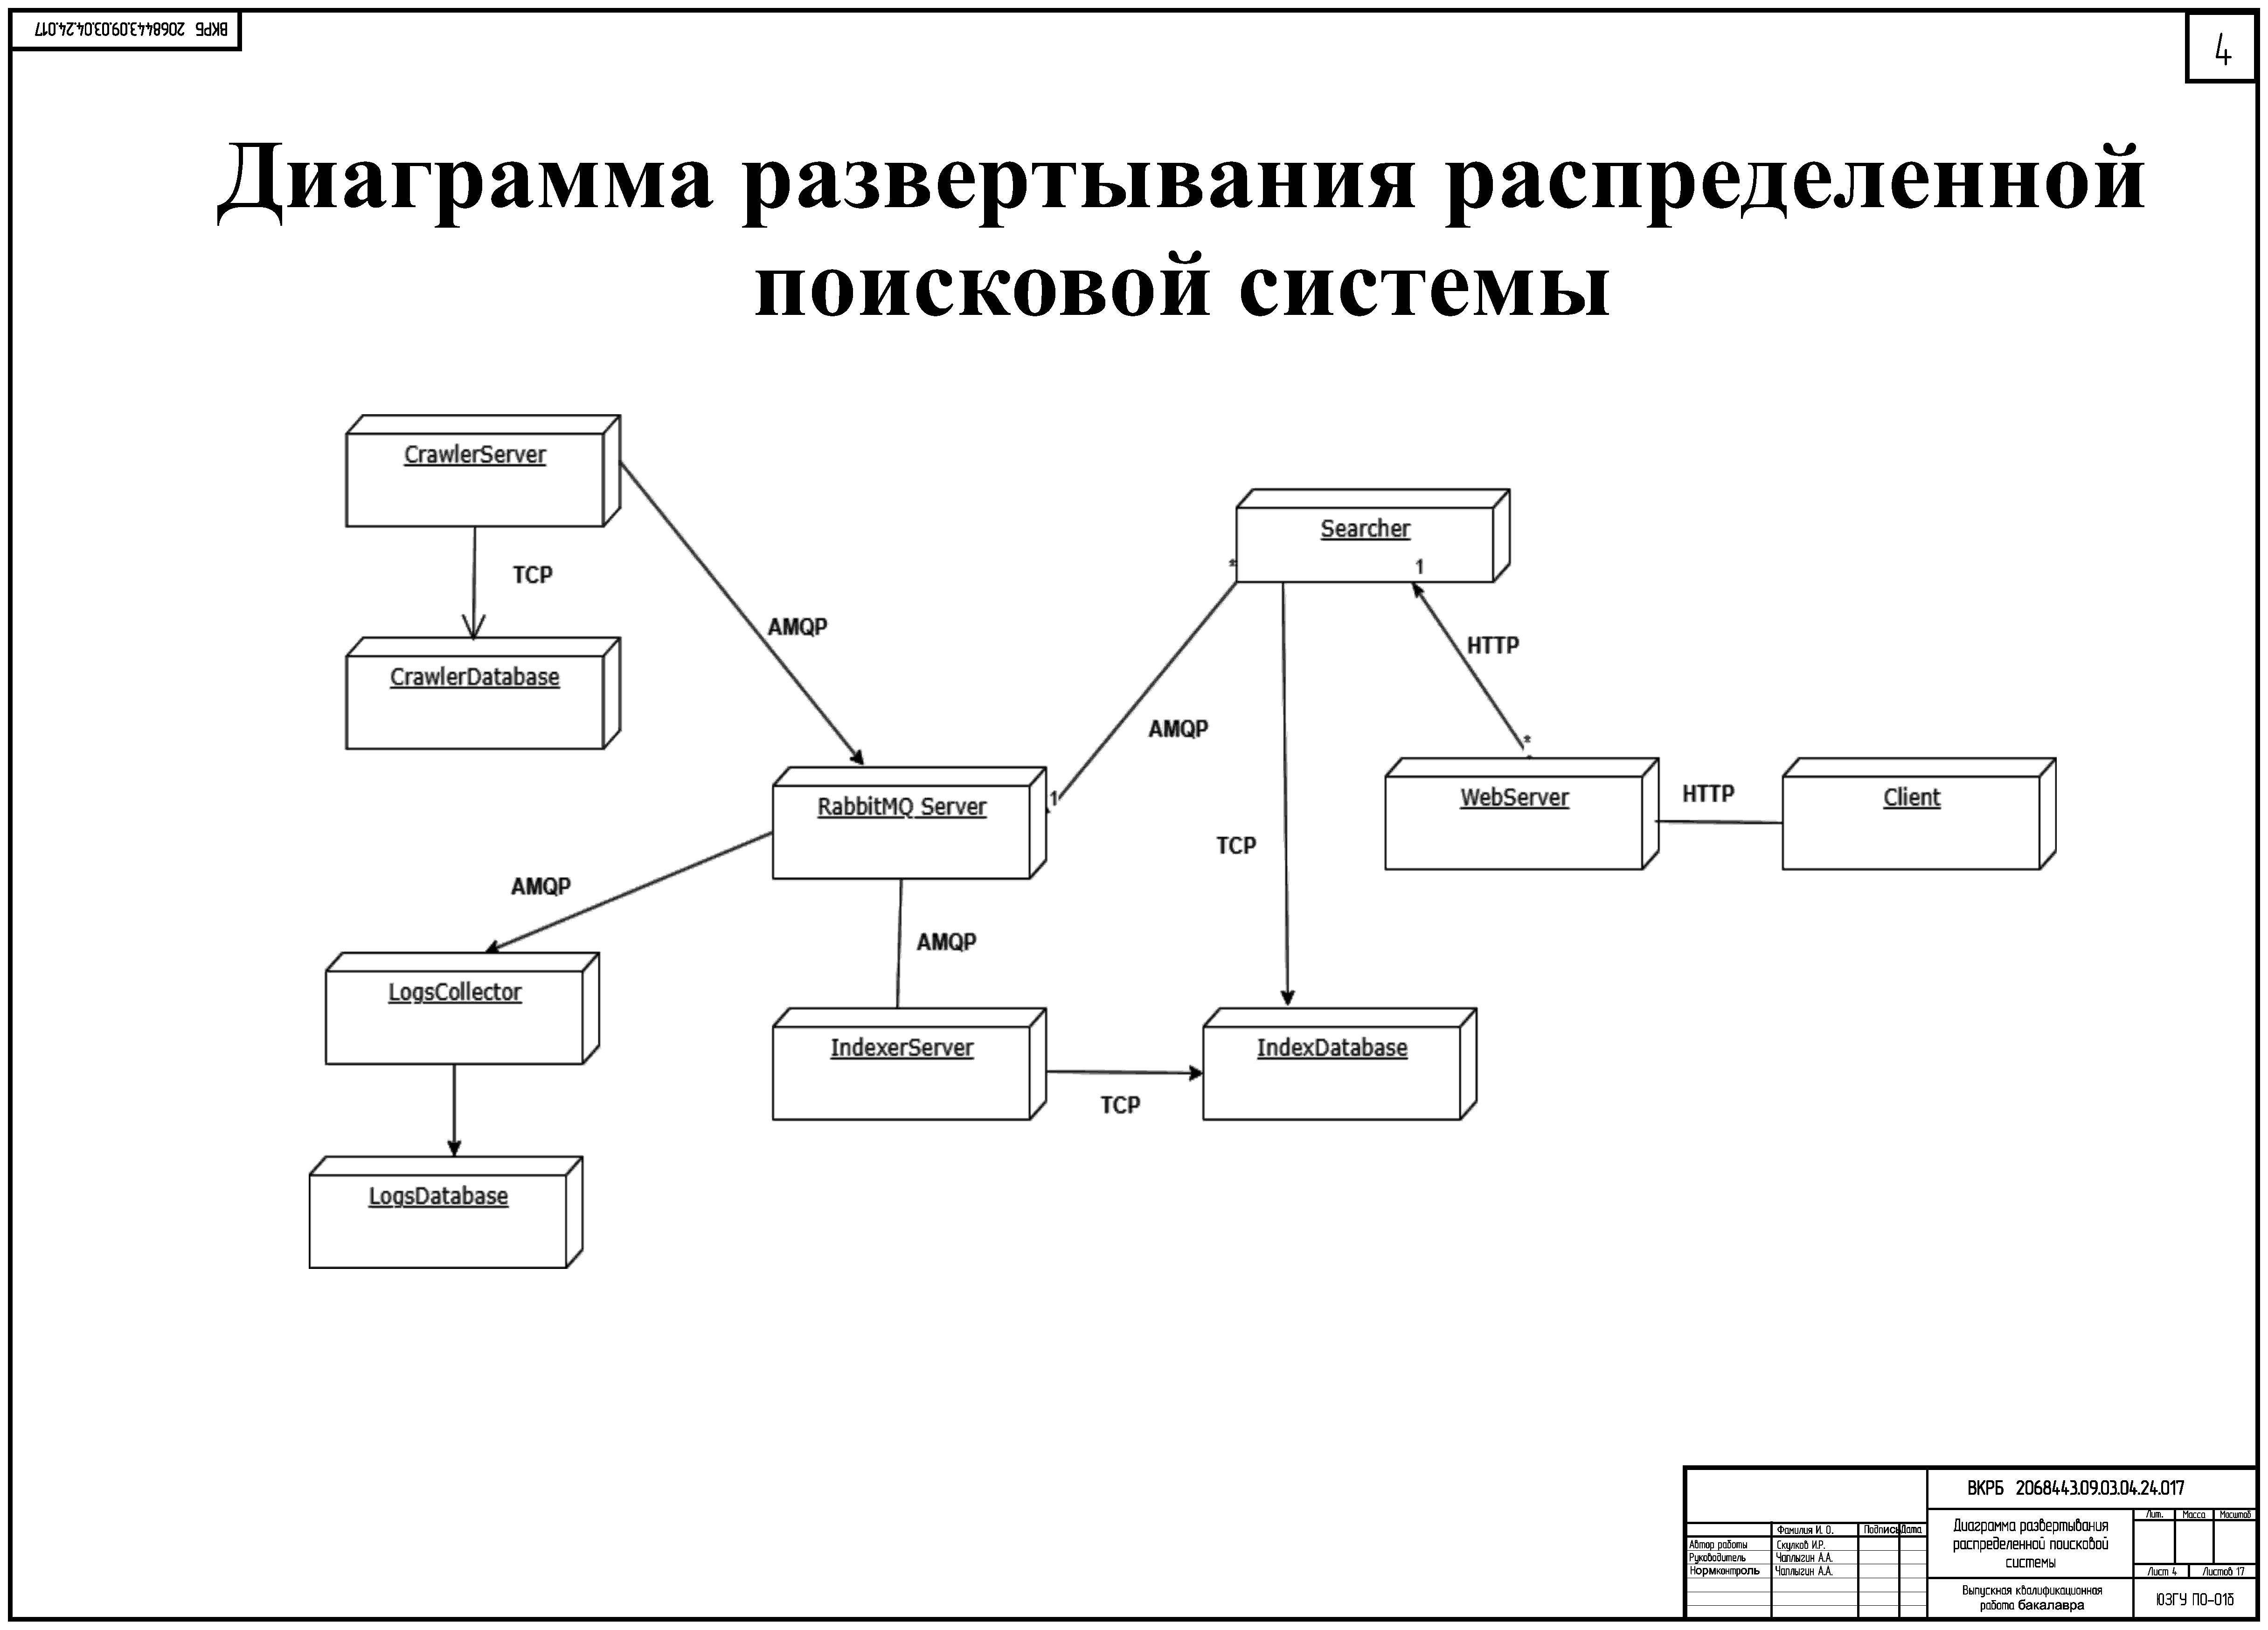
\includegraphics[width=0.82\linewidth]{posters/p4.eps}
    \заголовок{Диаграмма развертывания распределенной поисковой системы}
    \label{p4:image}      
\end{плакат}

\begin{плакат}
    
\includegraphics[width=0.82\linewidth]{posters/p5.eps}
    \заголовок{Диаграмма вариантов использования}
    \label{p5:image}      
\end{плакат}

\begin{плакат}
    
\includegraphics[width=0.82\linewidth]{posters/pr1.eps}
    \заголовок{Диаграмма компонентов поискового робота}
    \label{pr1:image}      
\end{плакат}

\begin{плакат}
    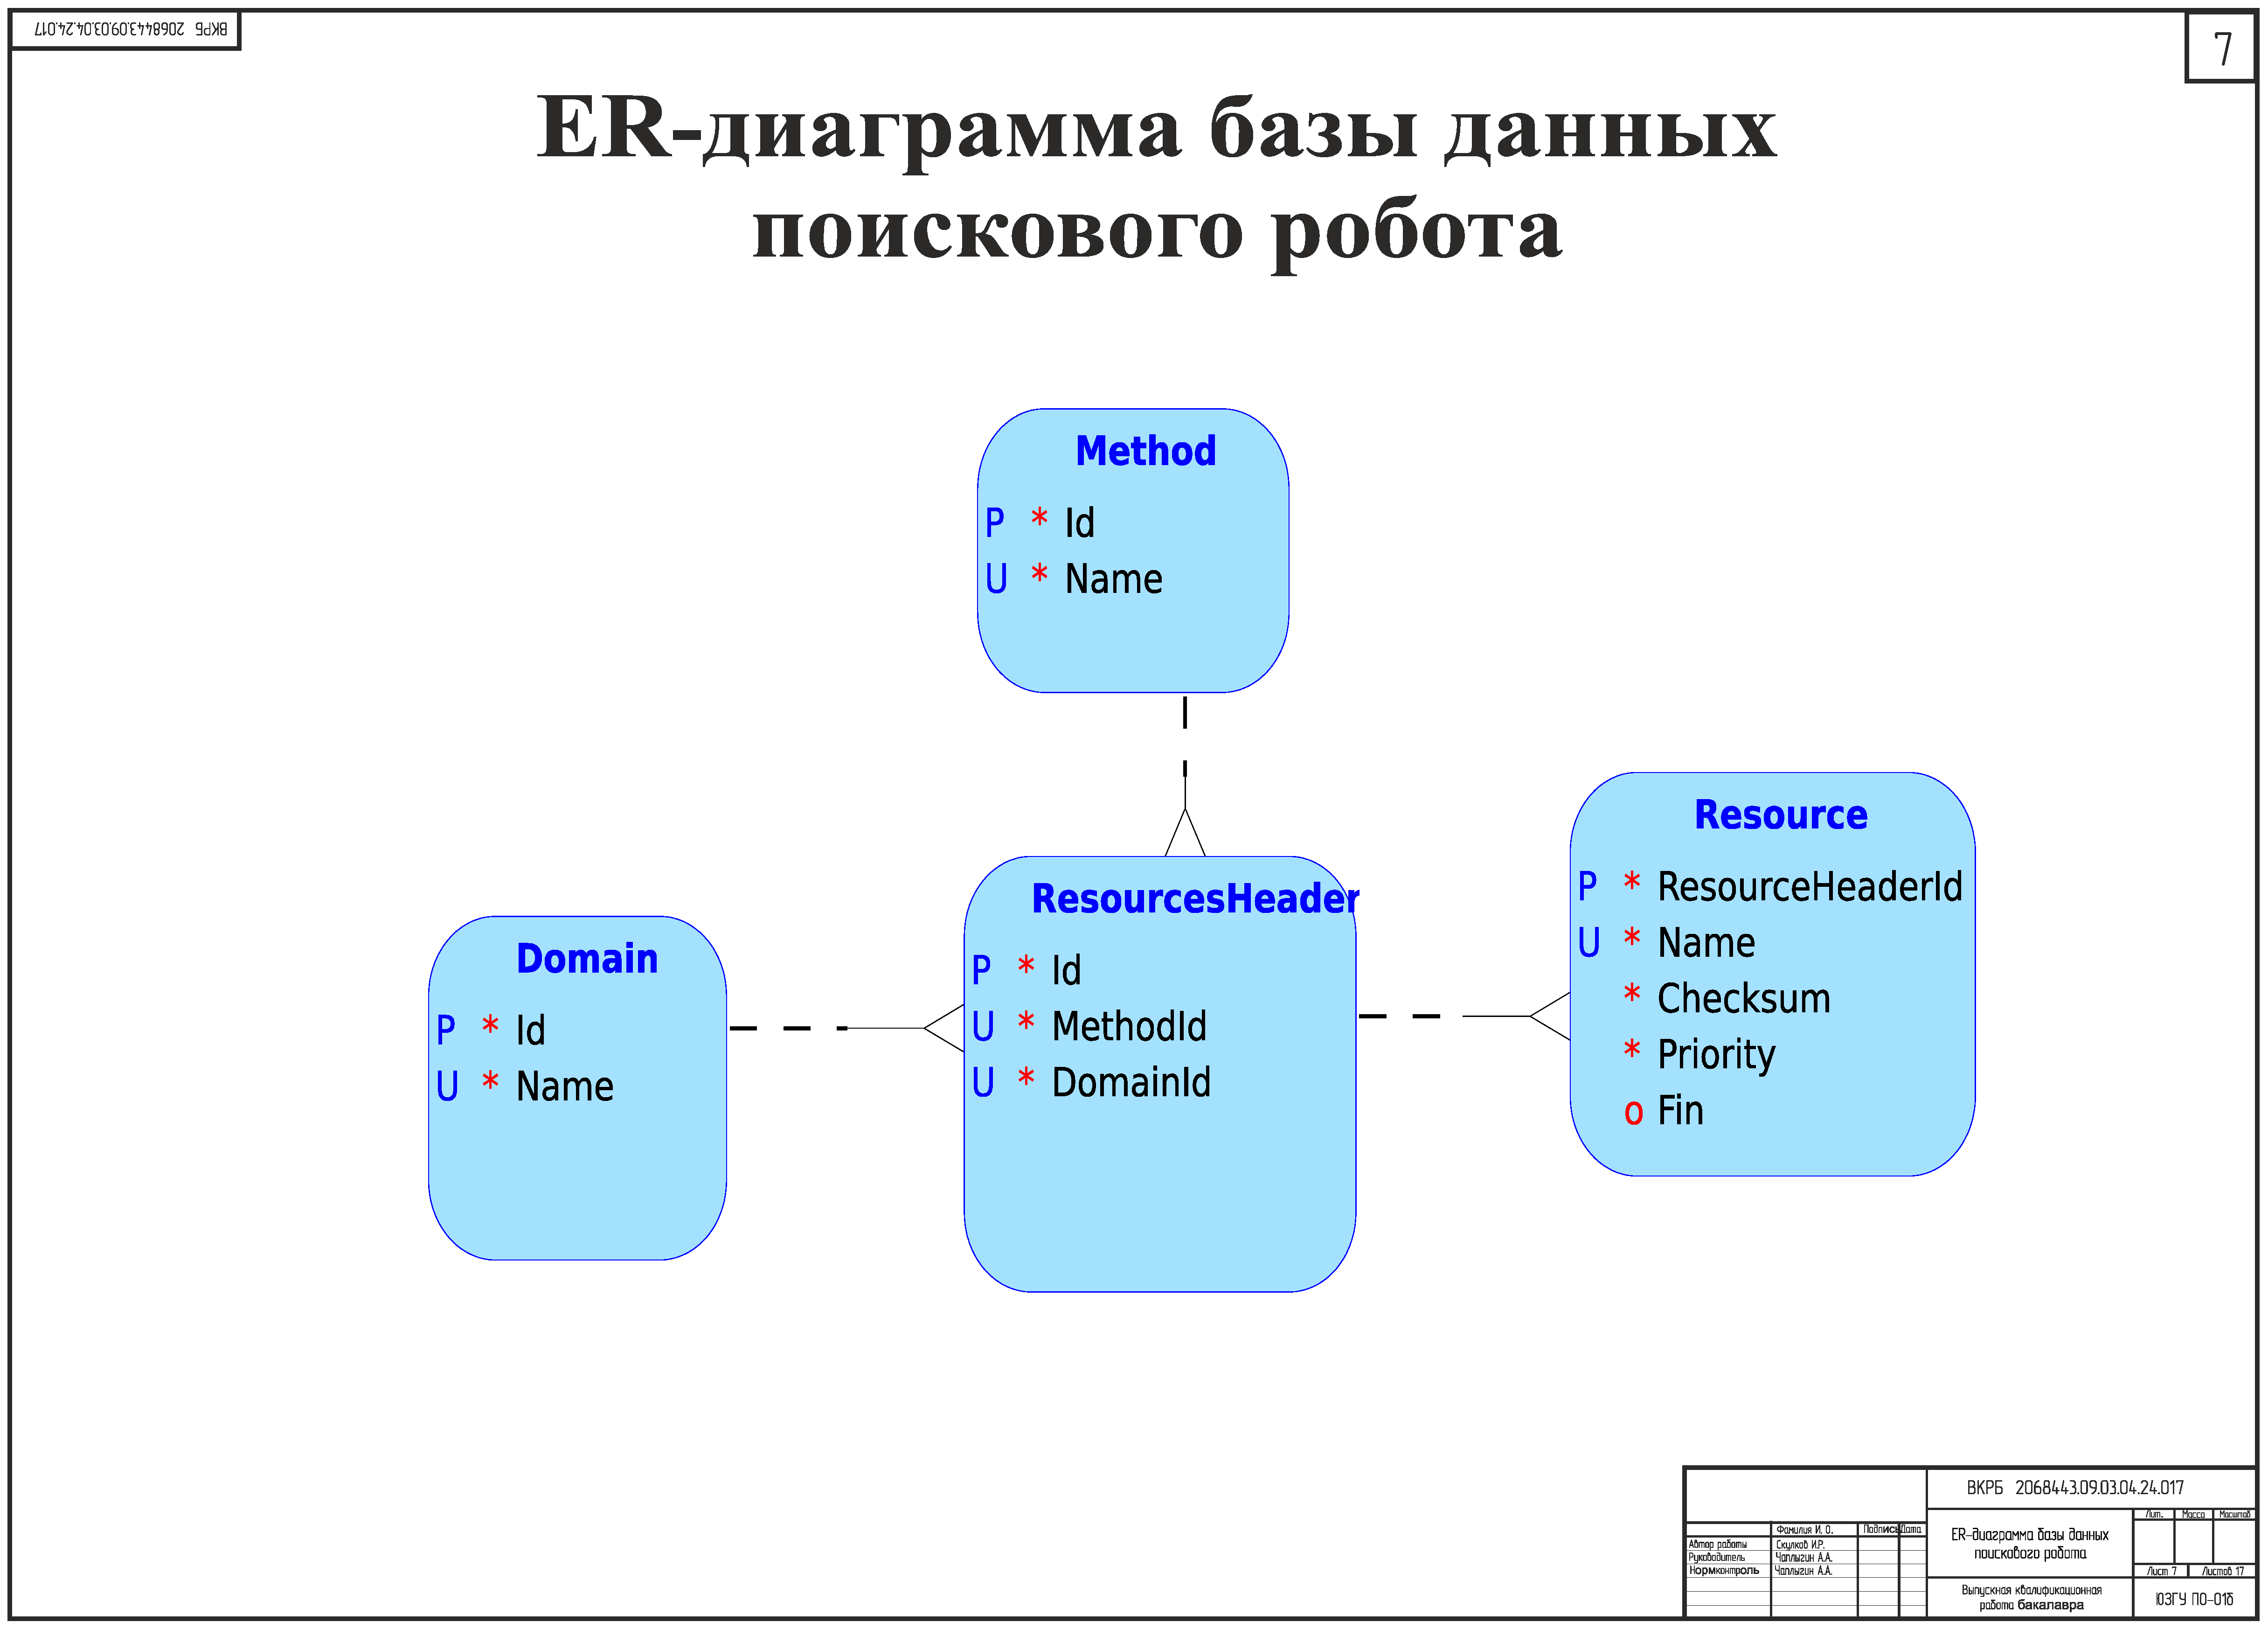
\includegraphics[width=0.82\linewidth]{posters/pr2.eps}
    \заголовок{ER-диаграмма базы данных поискового робота}
    \label{pr2:image}      
\end{плакат}

\begin{плакат}
    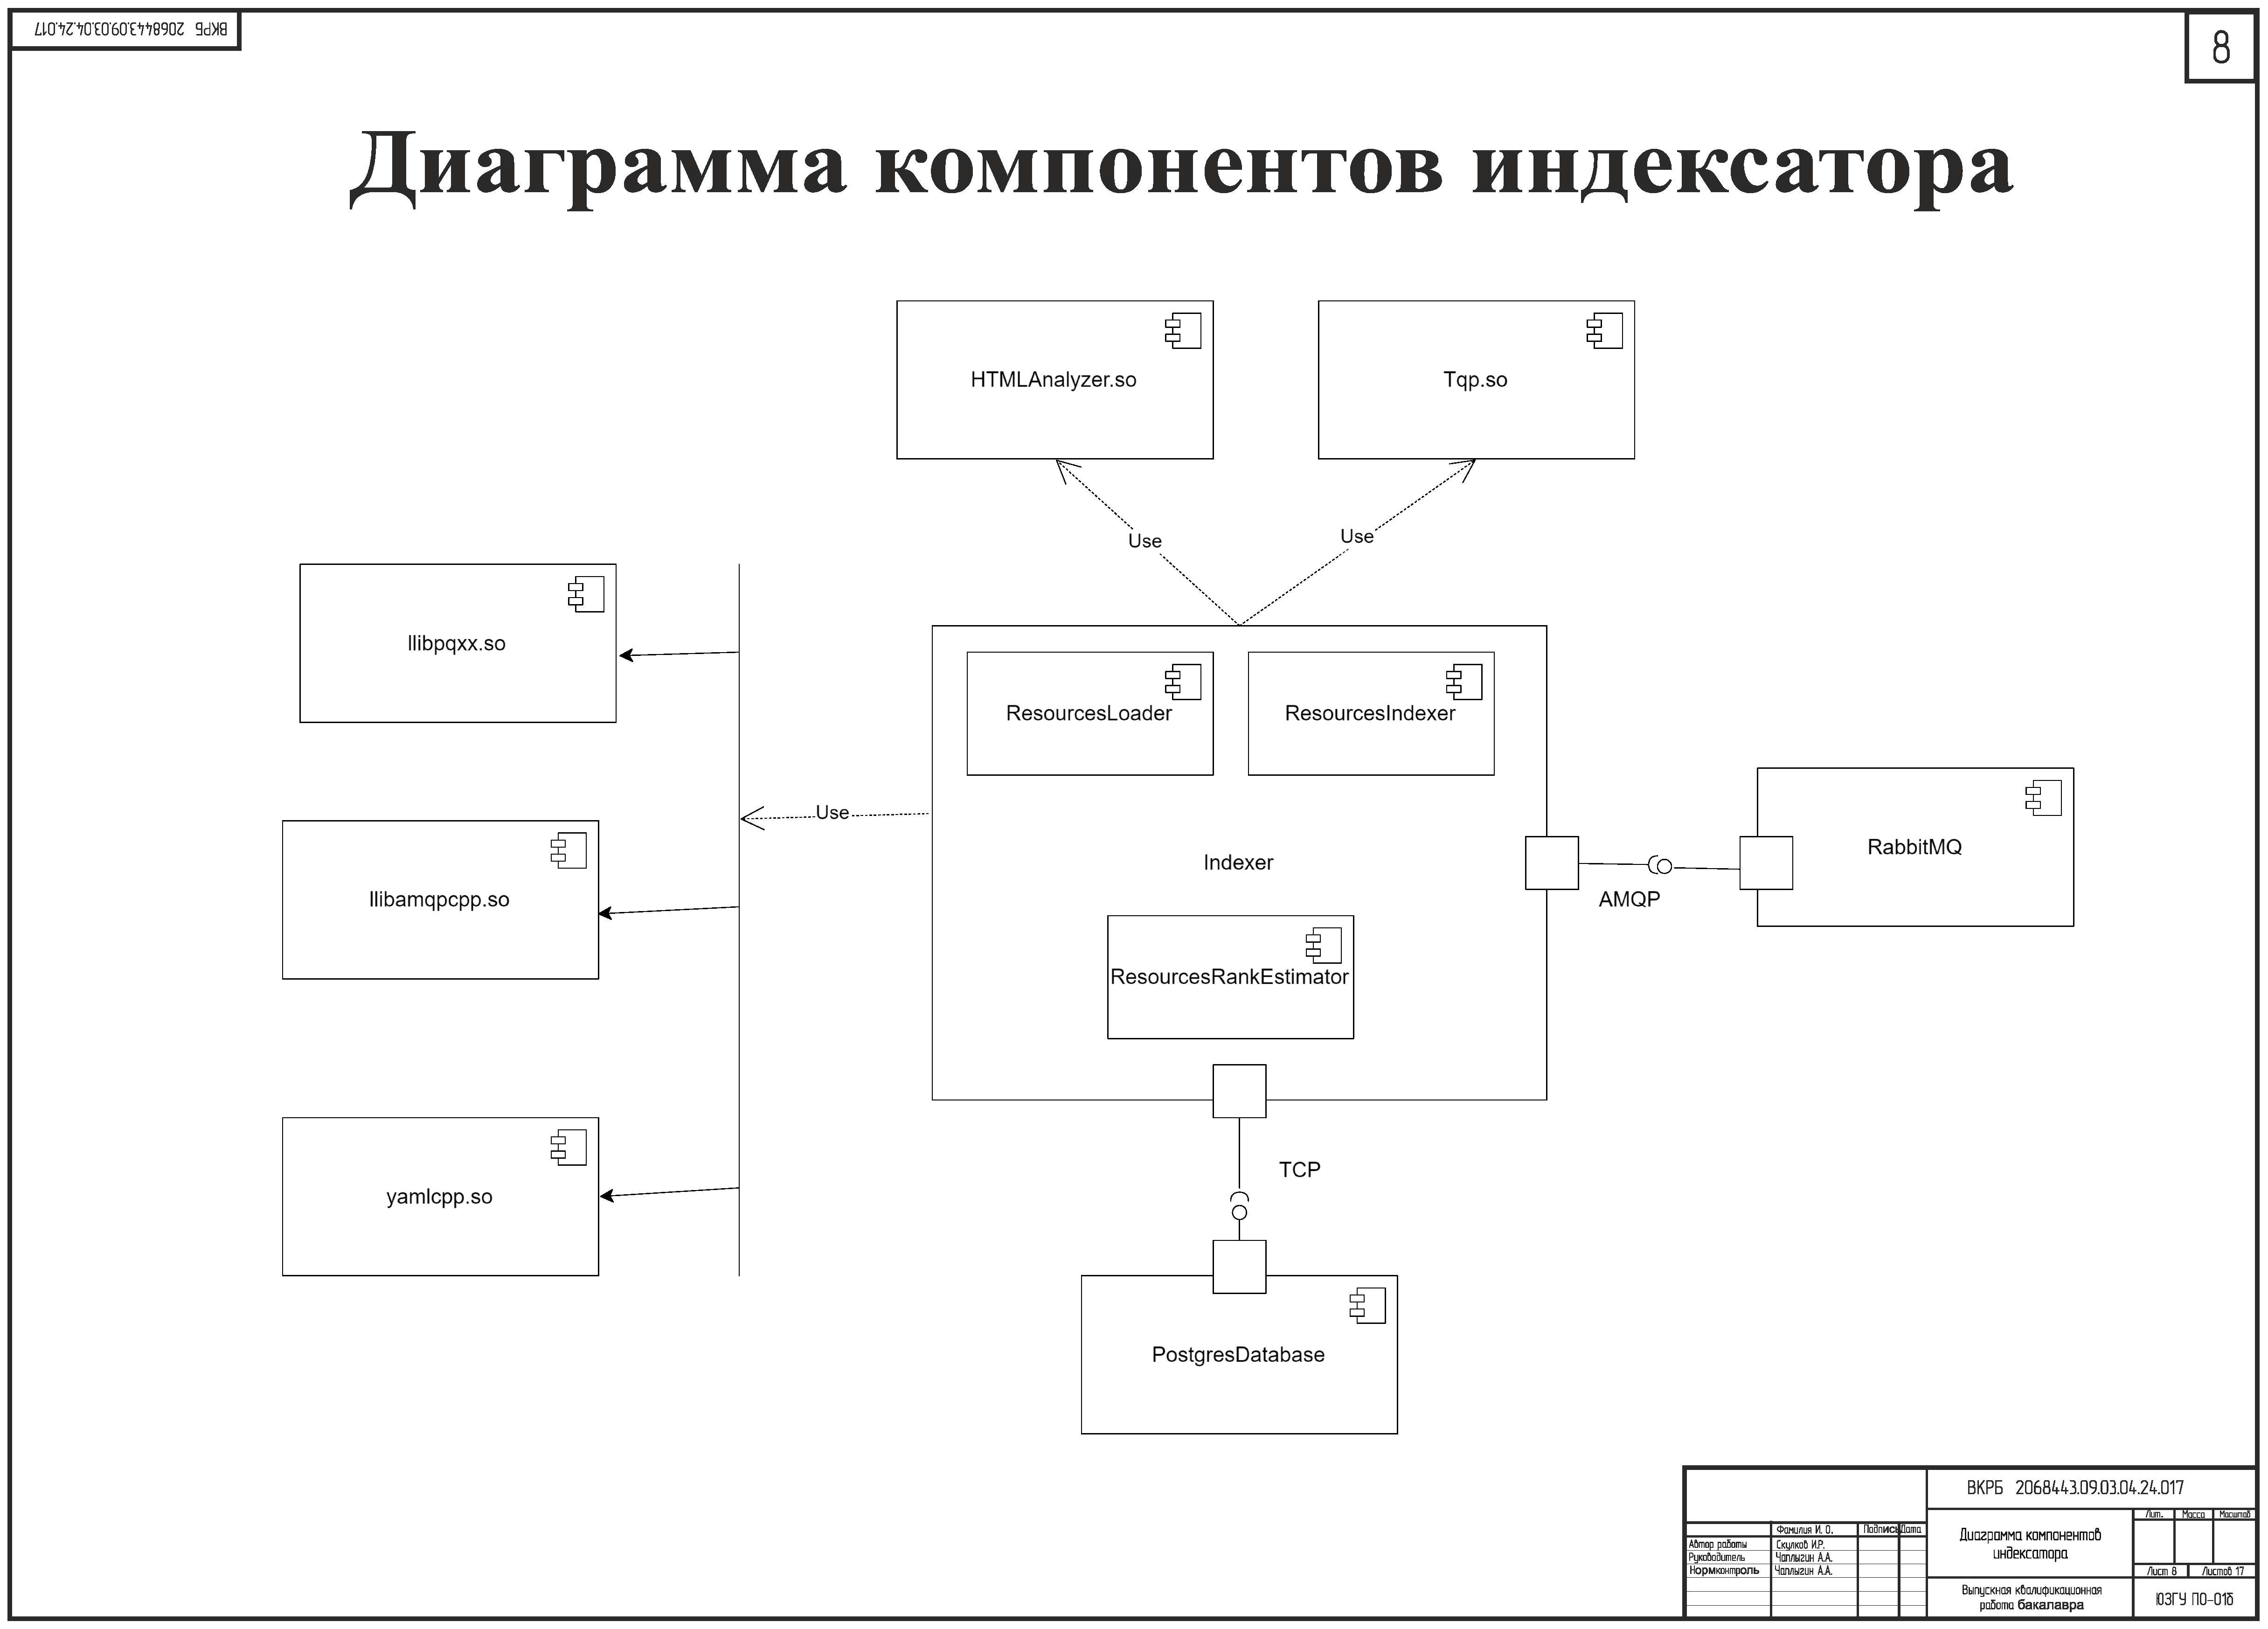
\includegraphics[width=0.82\linewidth]{posters/pi1.eps}
    \заголовок{Диаграмма компонентов индексатора}
    \label{pi1:image}      
\end{плакат}

\begin{плакат}
    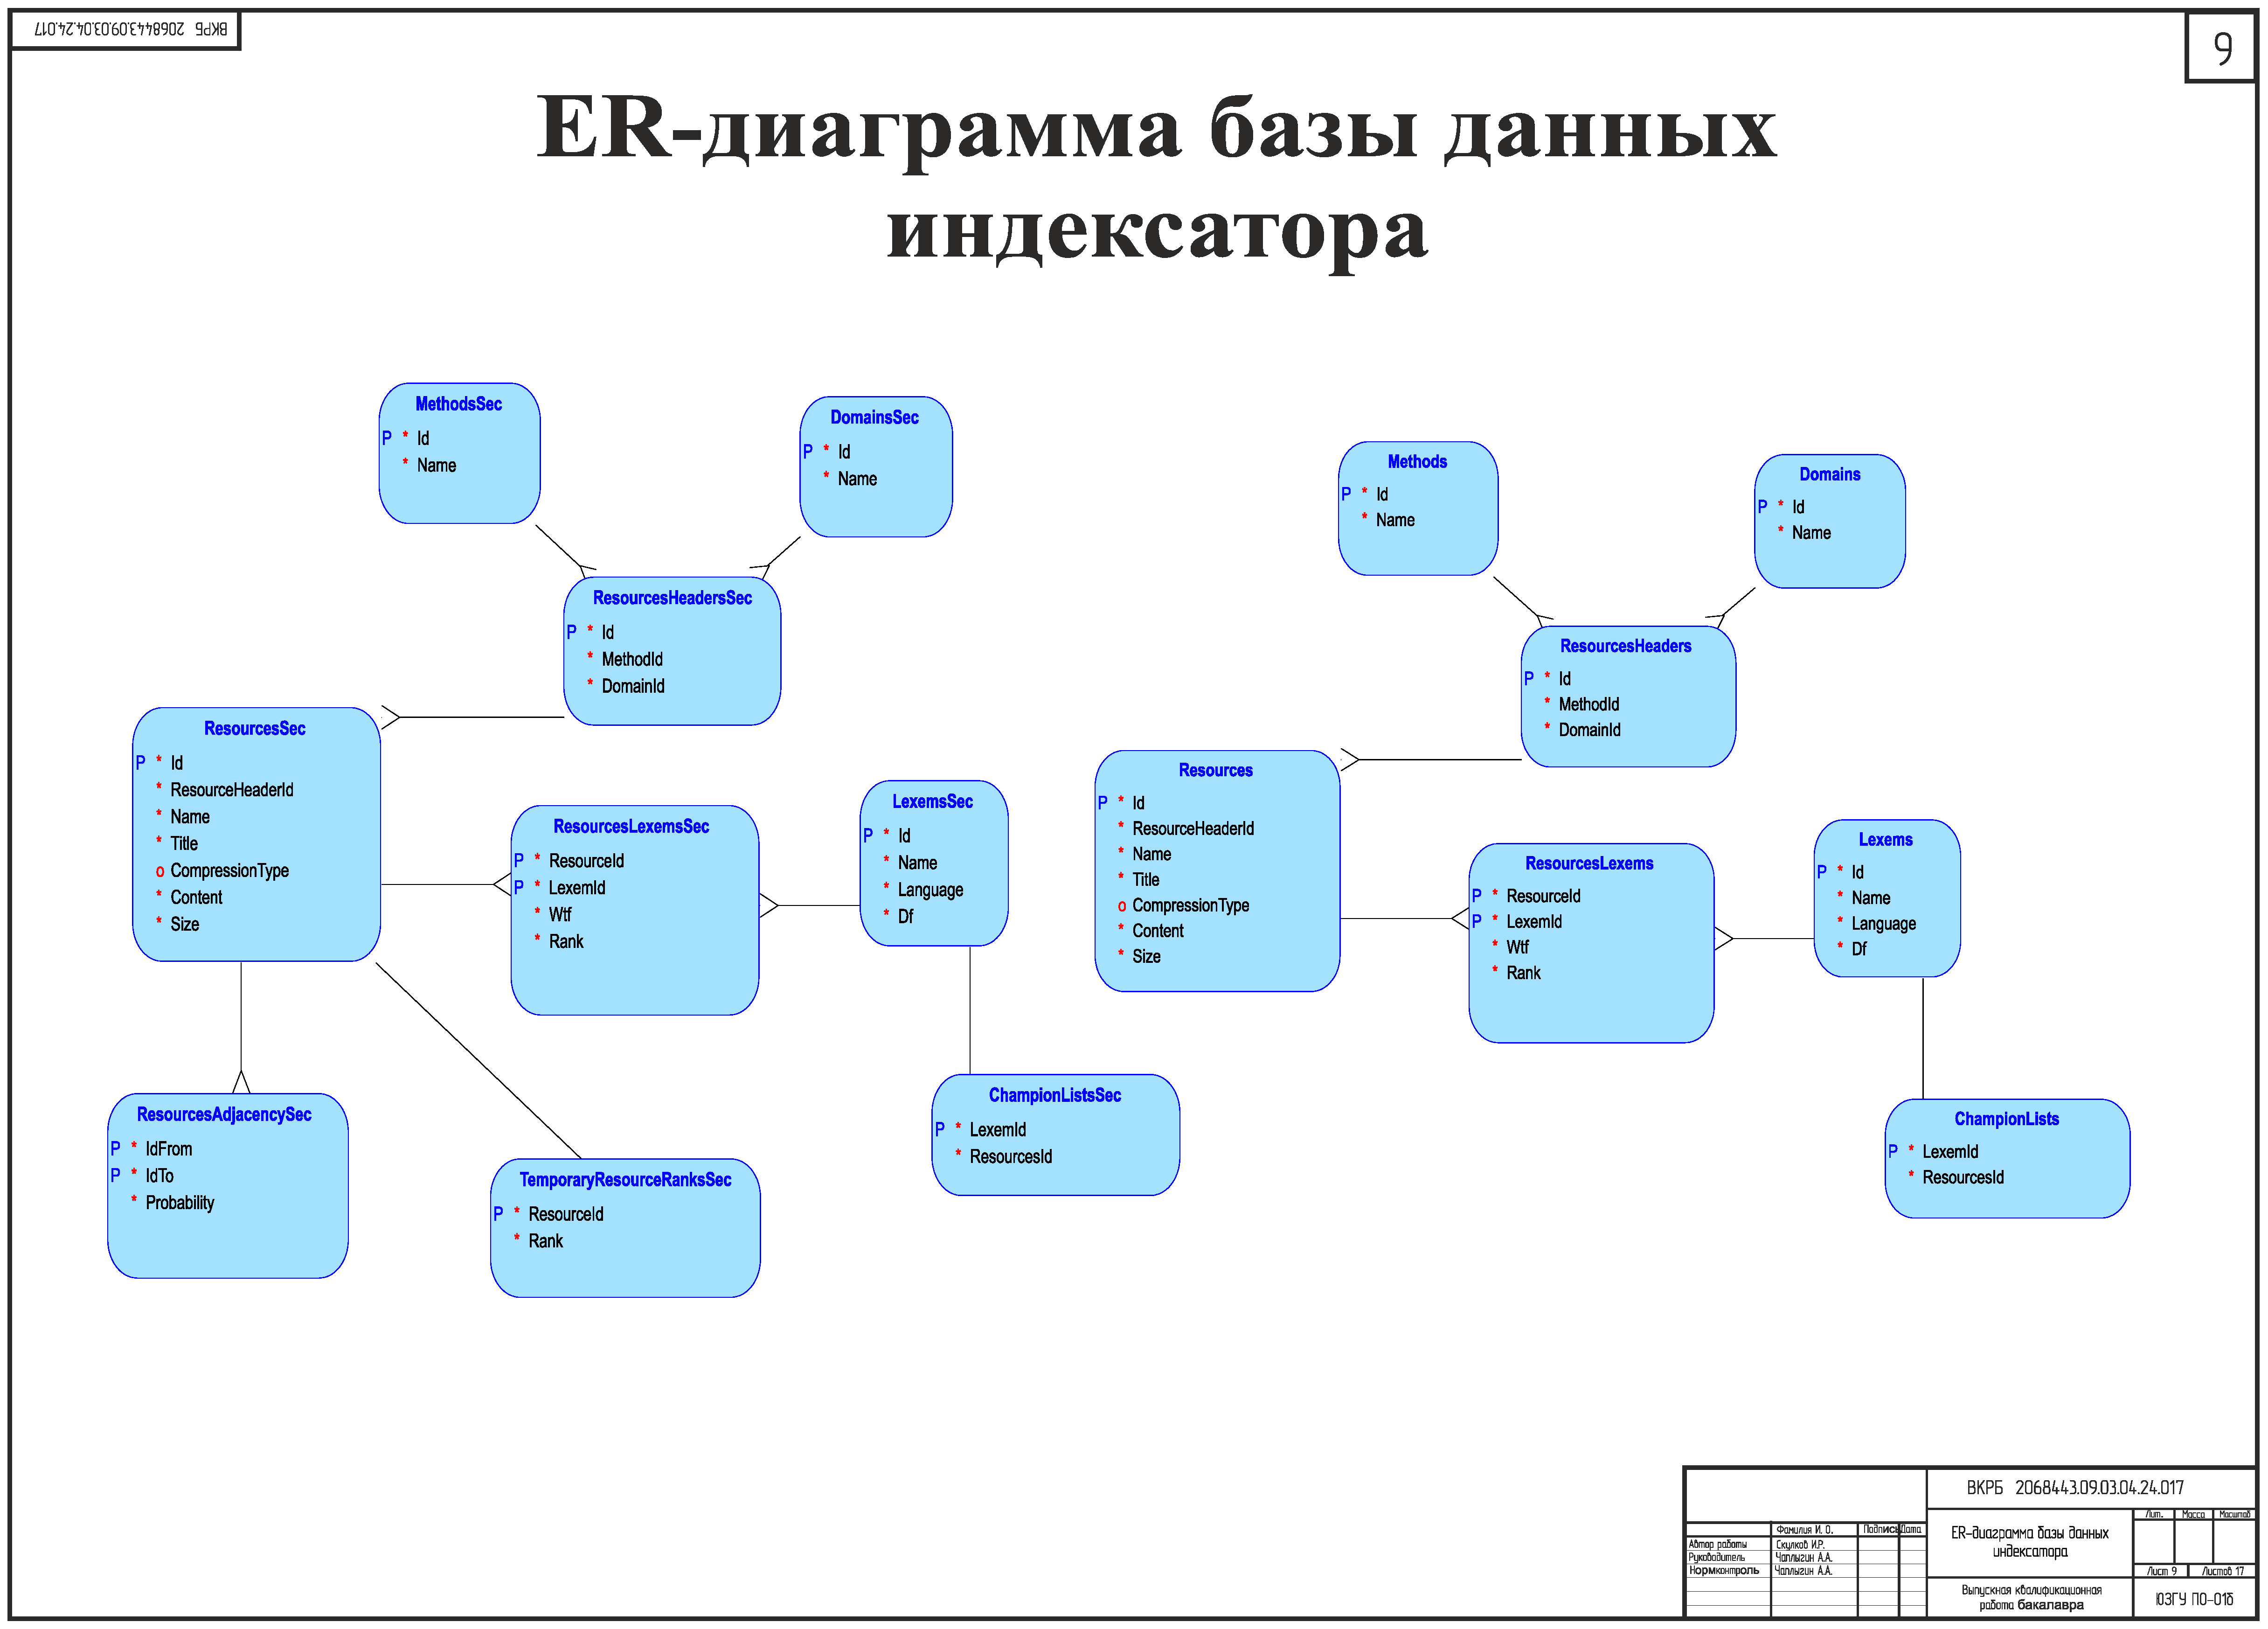
\includegraphics[width=0.82\linewidth]{posters/pi2.eps}
    \заголовок{ER-диаграмма базы данных индексатора}
    \label{pi2:image}      
\end{плакат}

\begin{плакат}
    
\includegraphics[width=0.82\linewidth]{posters/ps1.eps}
    \заголовок{Диаграмма компонентов поискового интерфейса}
    \label{ps1:image}      
\end{плакат}

\begin{плакат}
    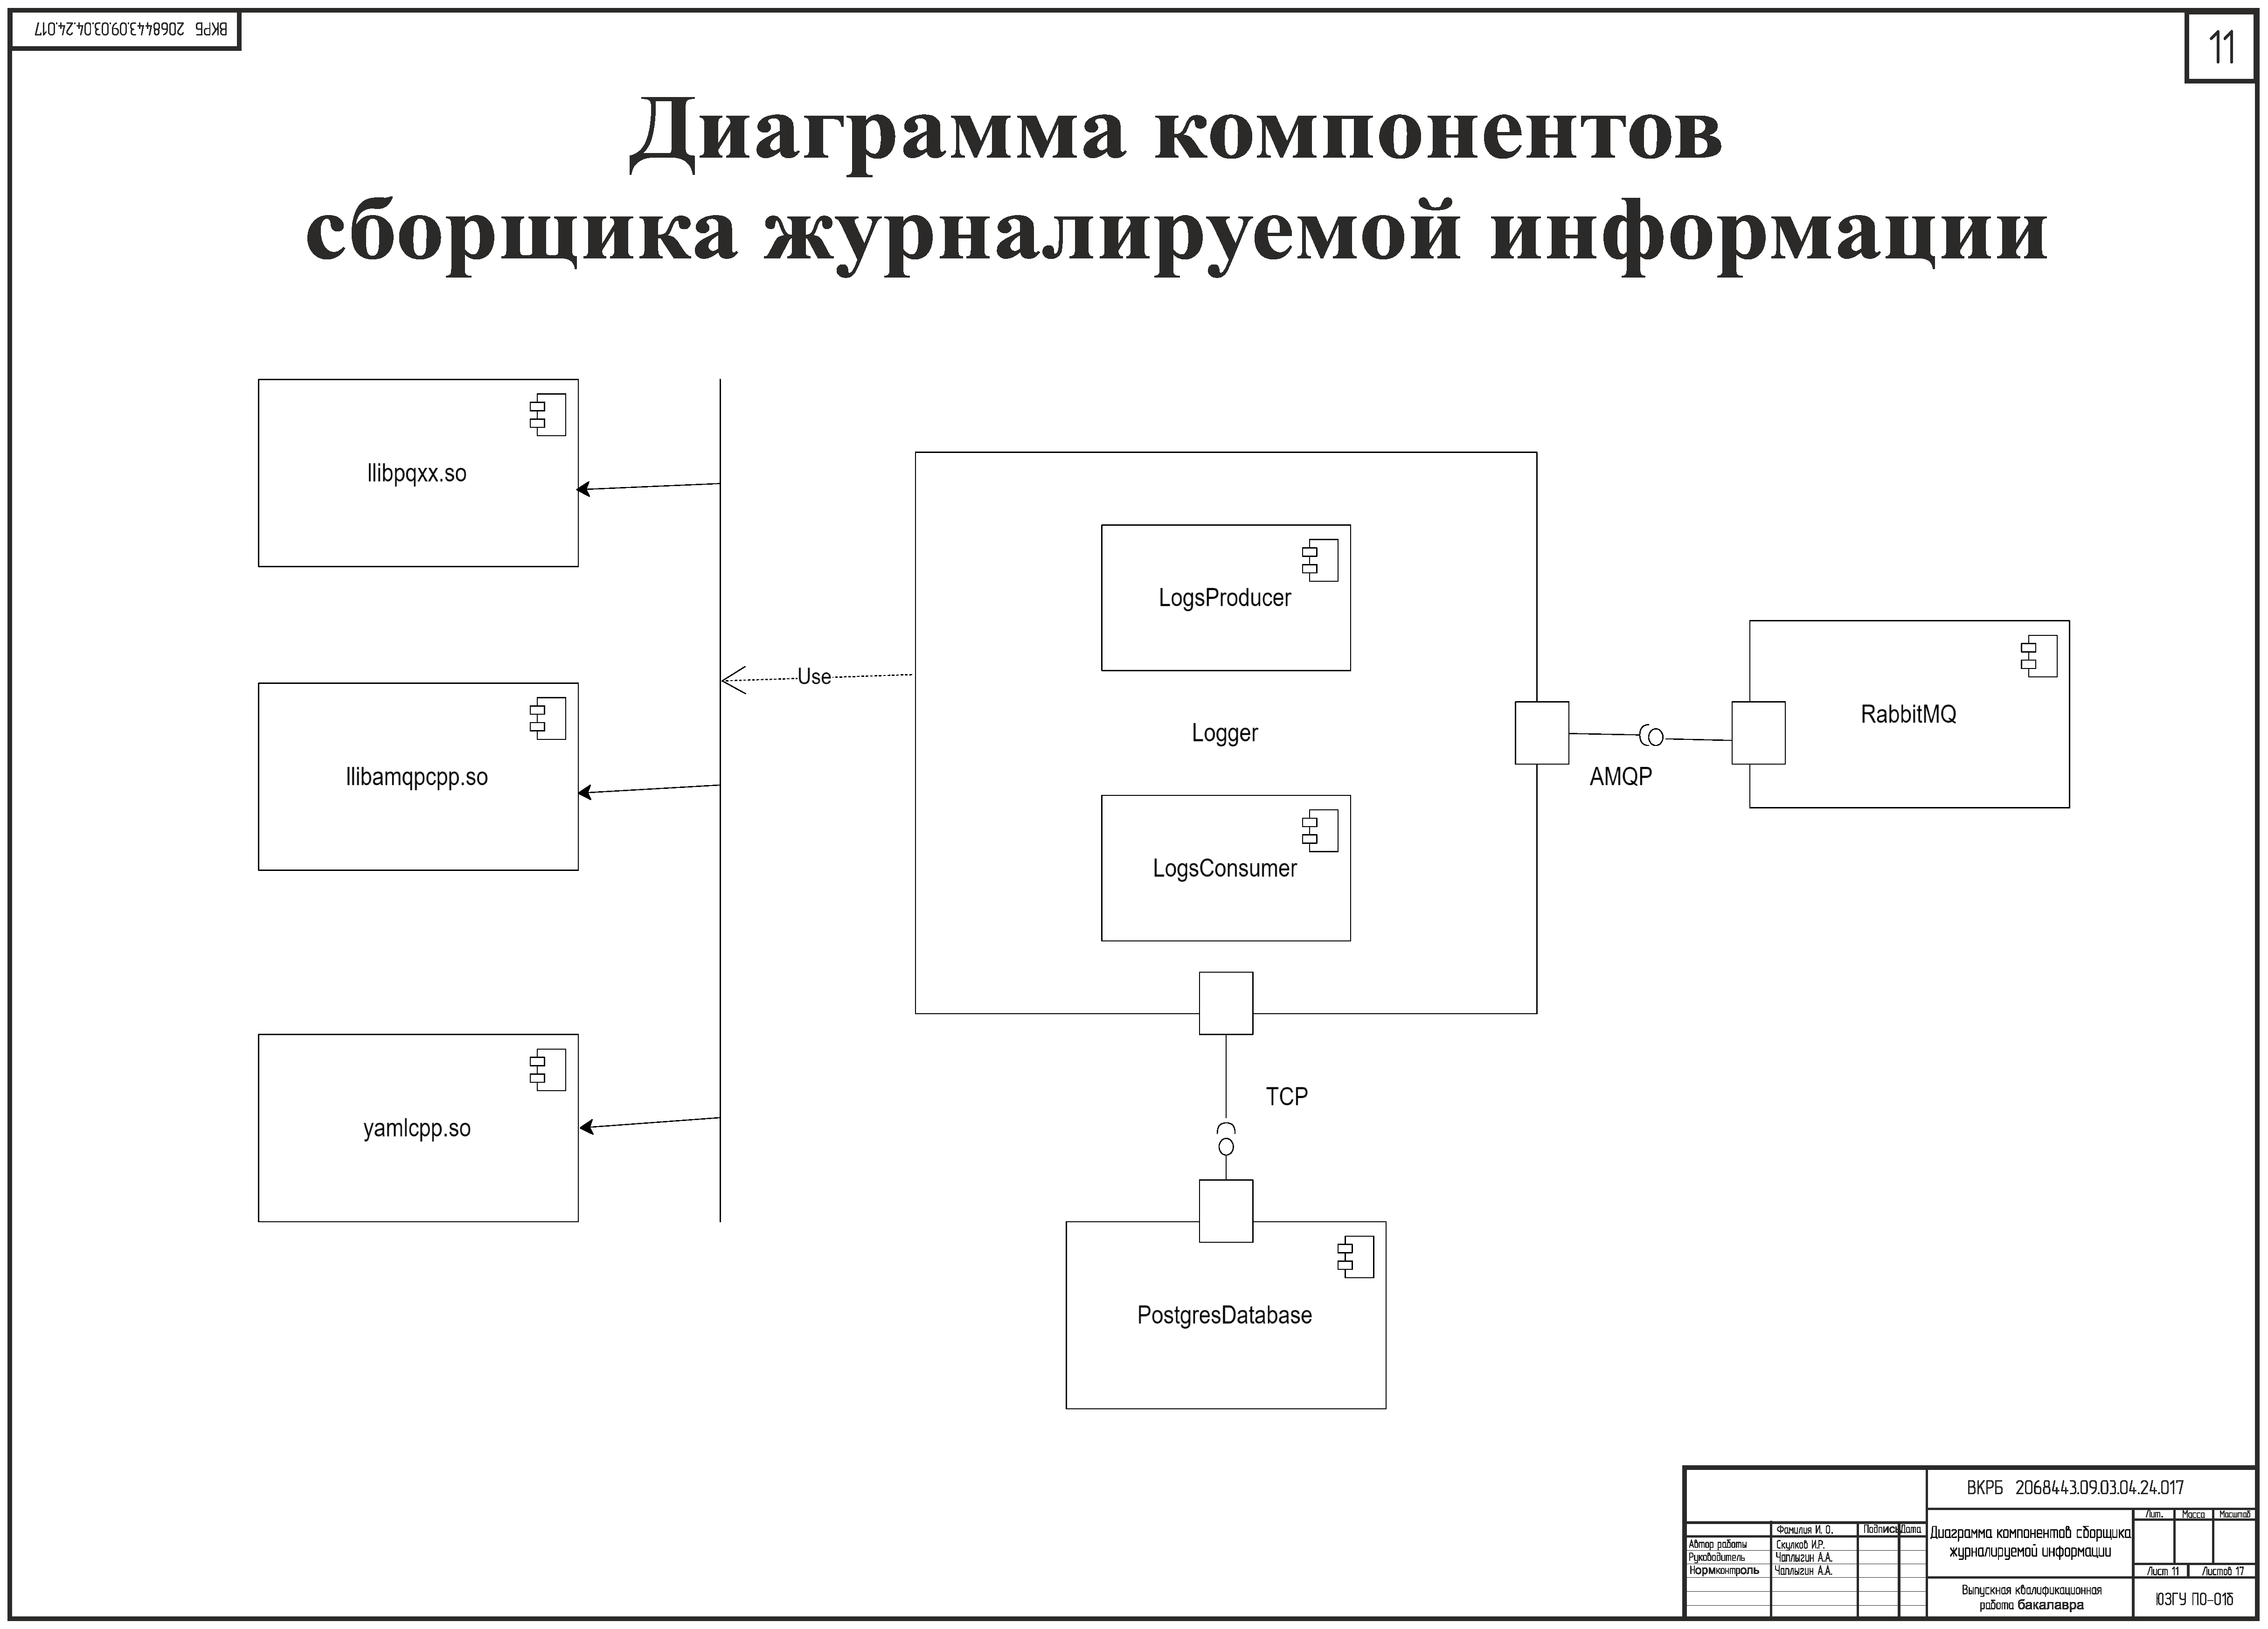
\includegraphics[width=0.82\linewidth]{posters/pl1.eps}
    \заголовок{Диаграмма компонентов сборщика журналируемой информации}
    \label{pl1:image}      
\end{плакат}

\begin{плакат}
    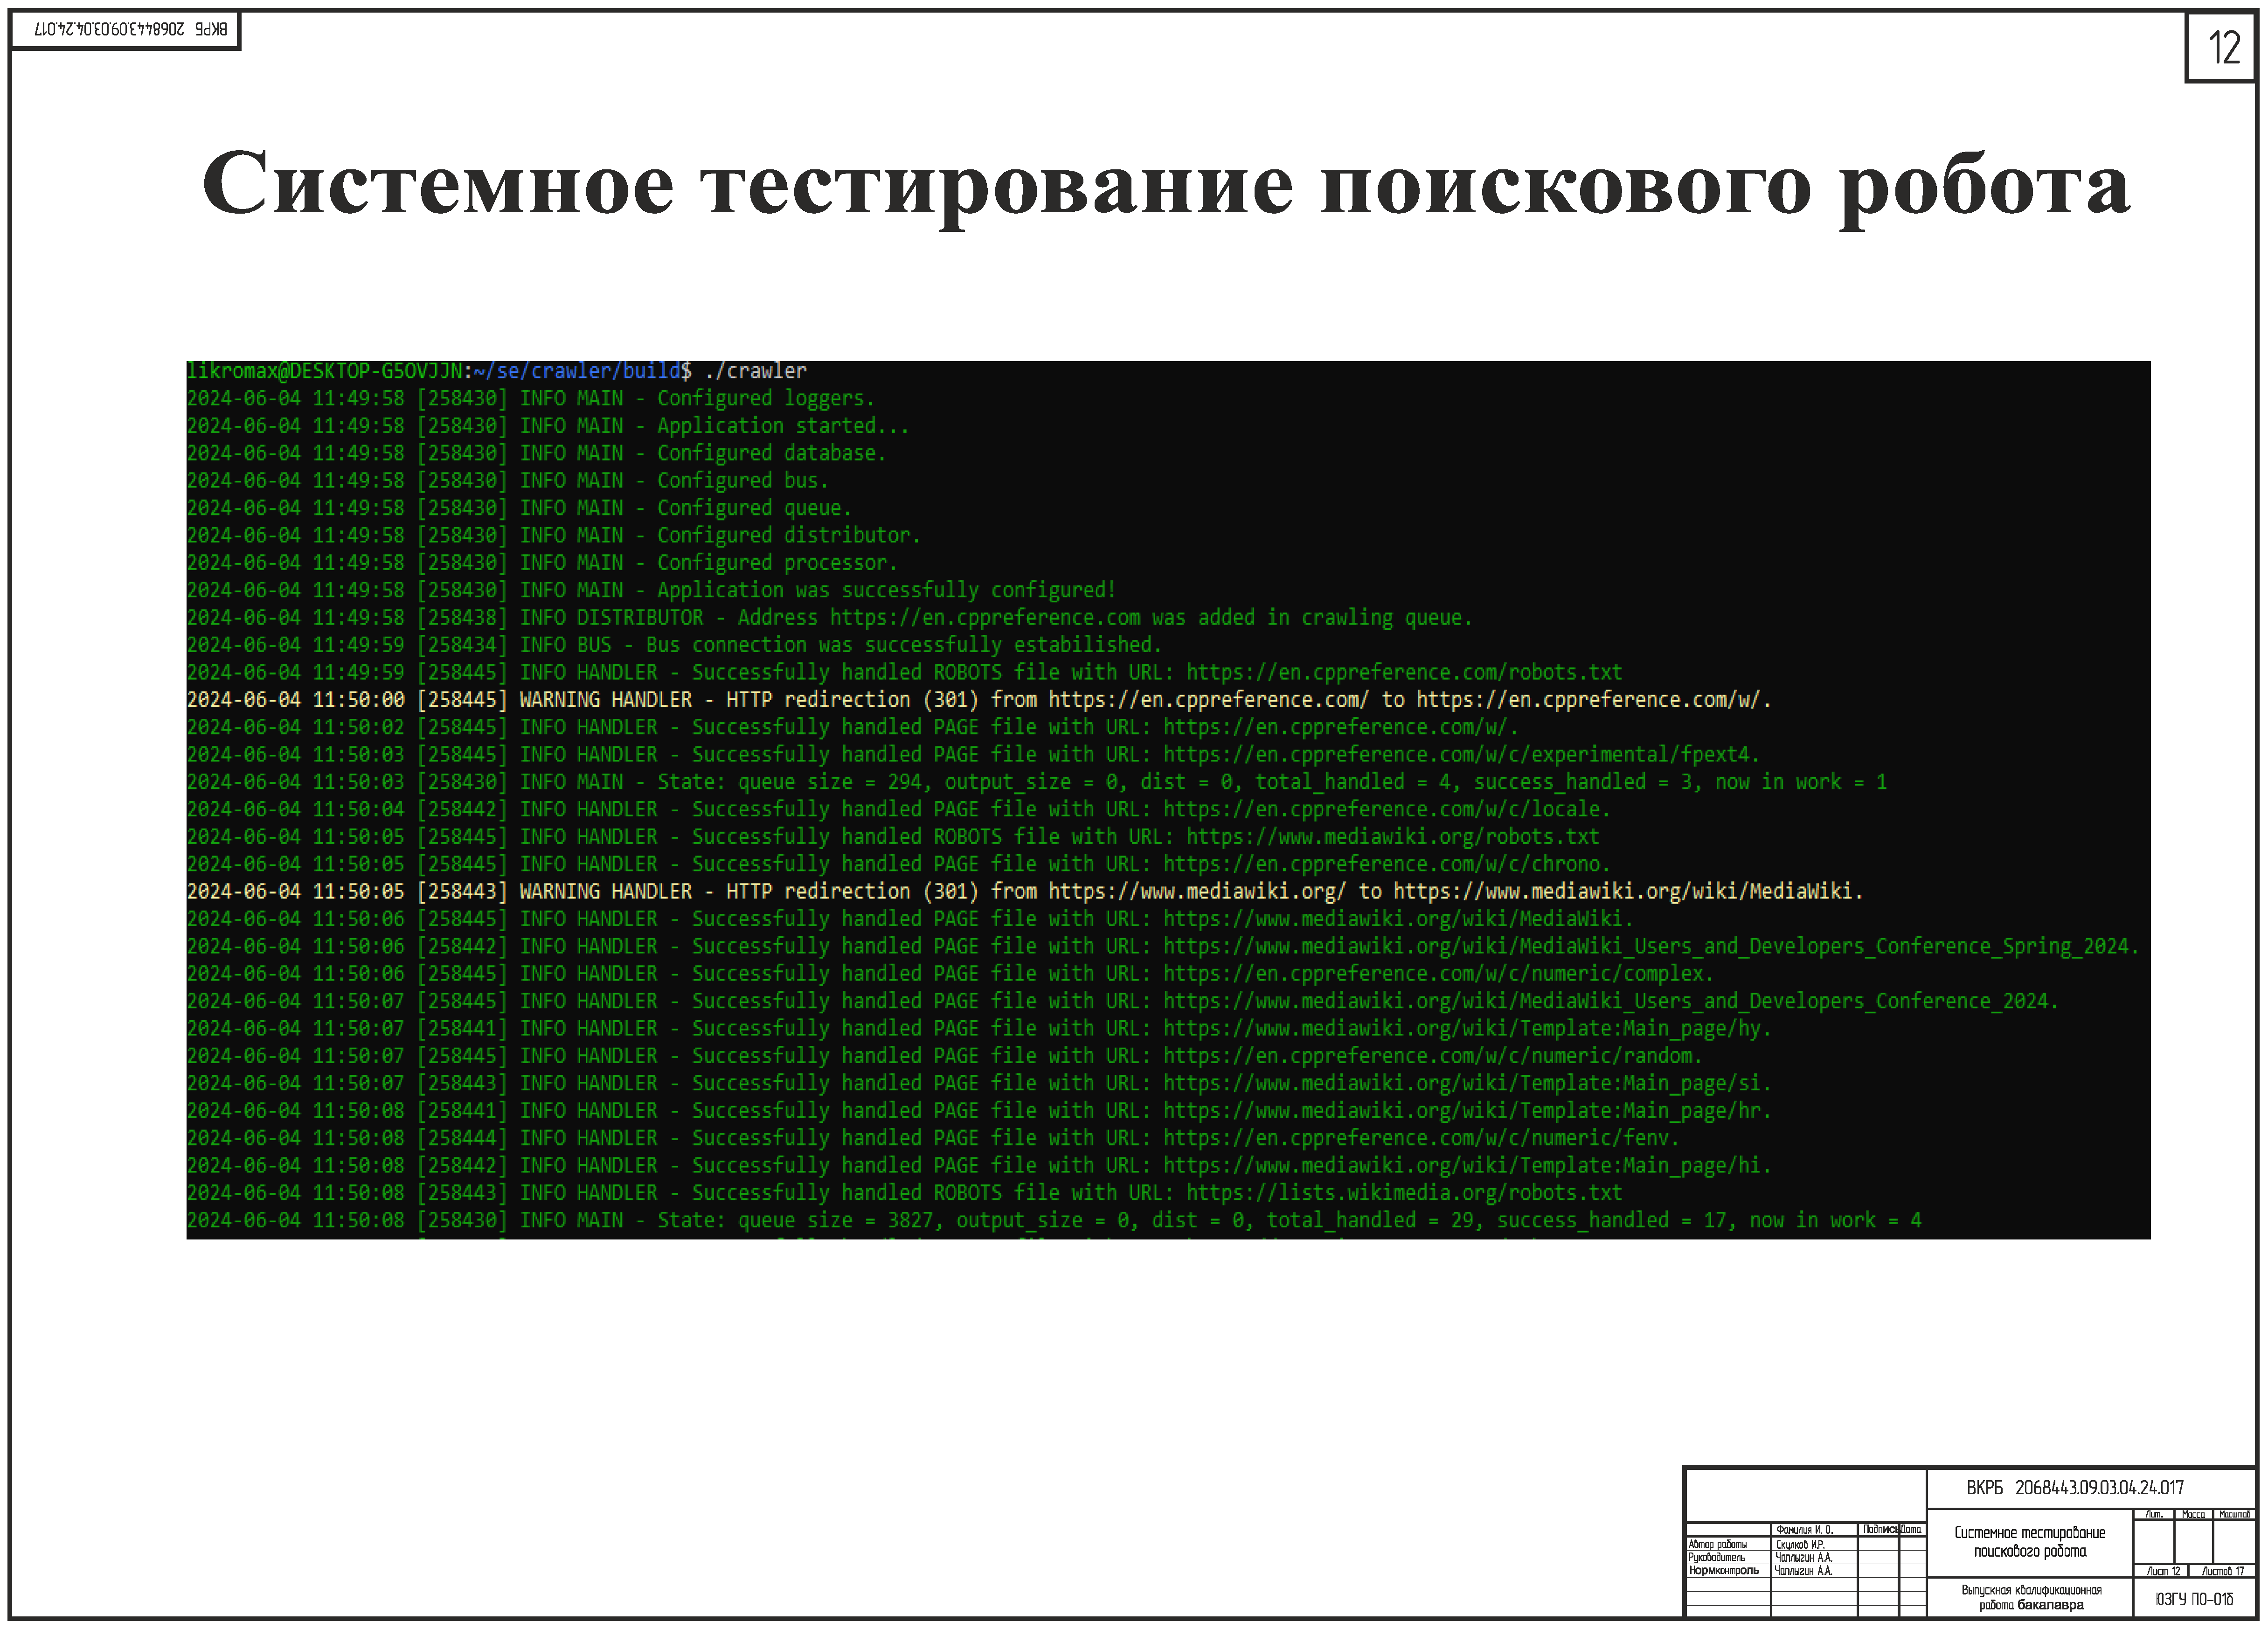
\includegraphics[width=0.82\linewidth]{posters/ptr.eps}
    \заголовок{Системное тестирование поискового робота}
    \label{ptr:image}      
\end{плакат}

\begin{плакат}
    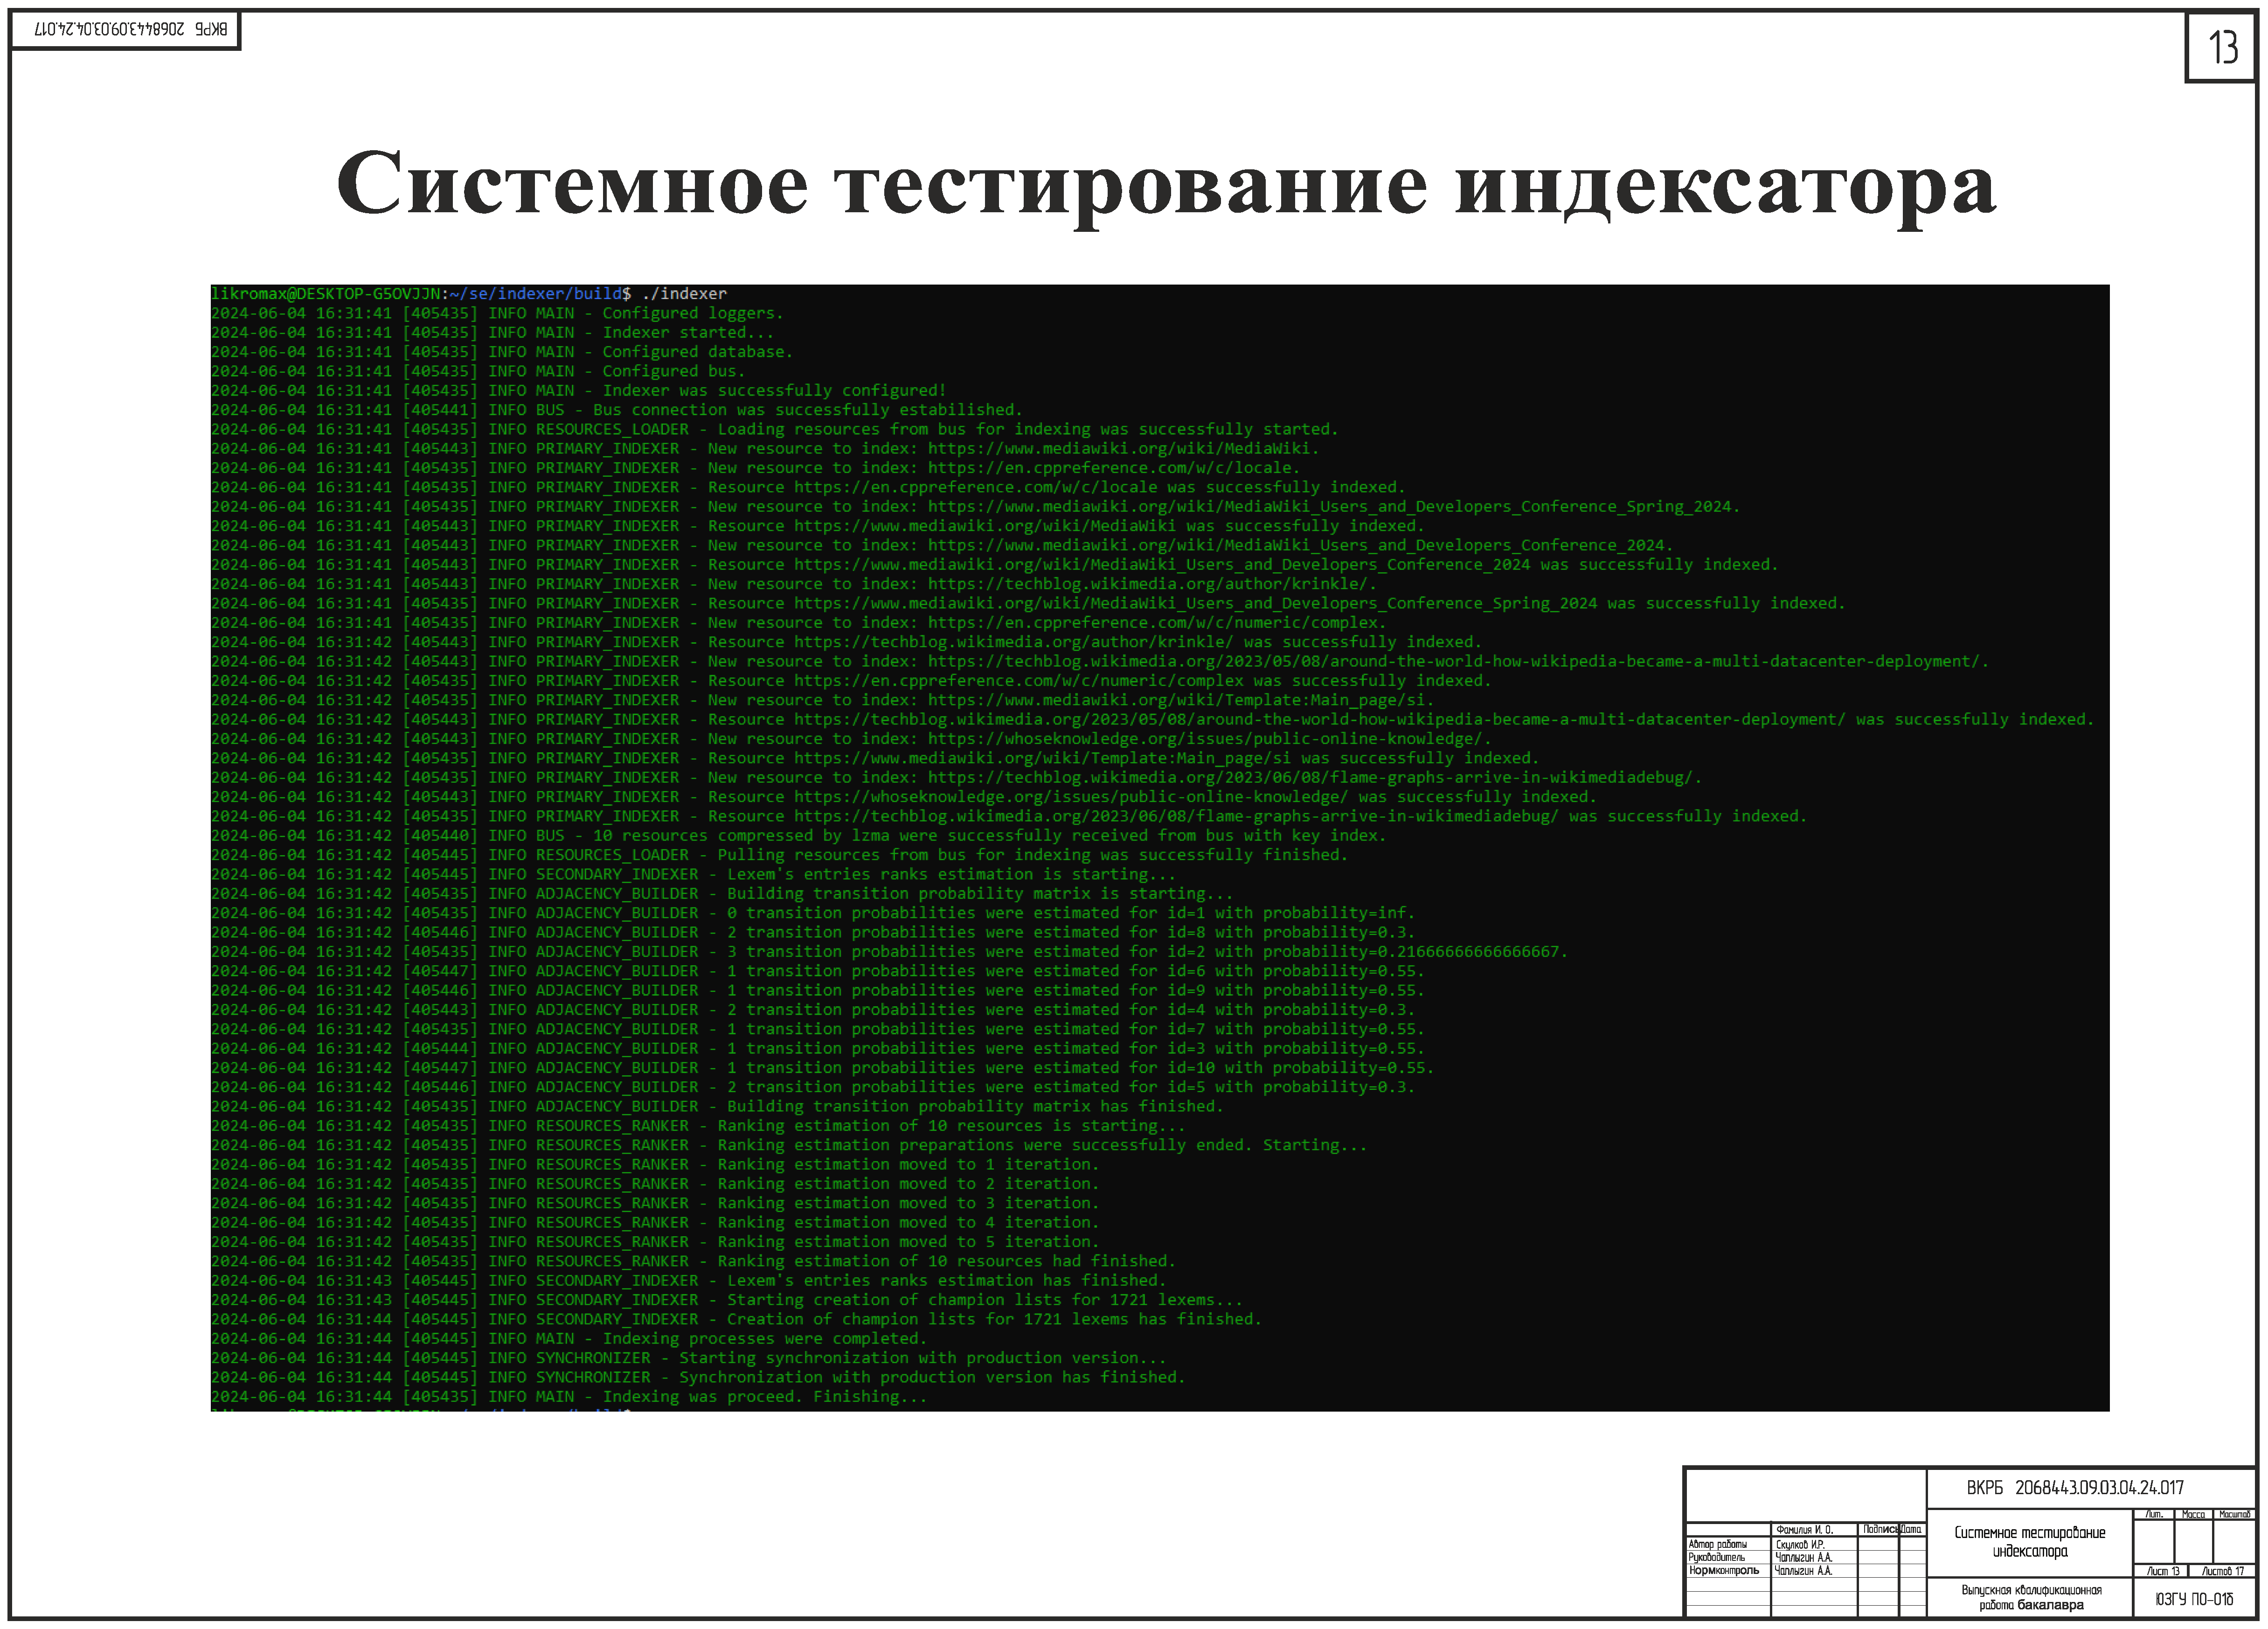
\includegraphics[width=0.82\linewidth]{posters/pti.eps}
    \заголовок{Системное тестирование индексатора}
    \label{pti:image}      
\end{плакат}

\begin{плакат}
    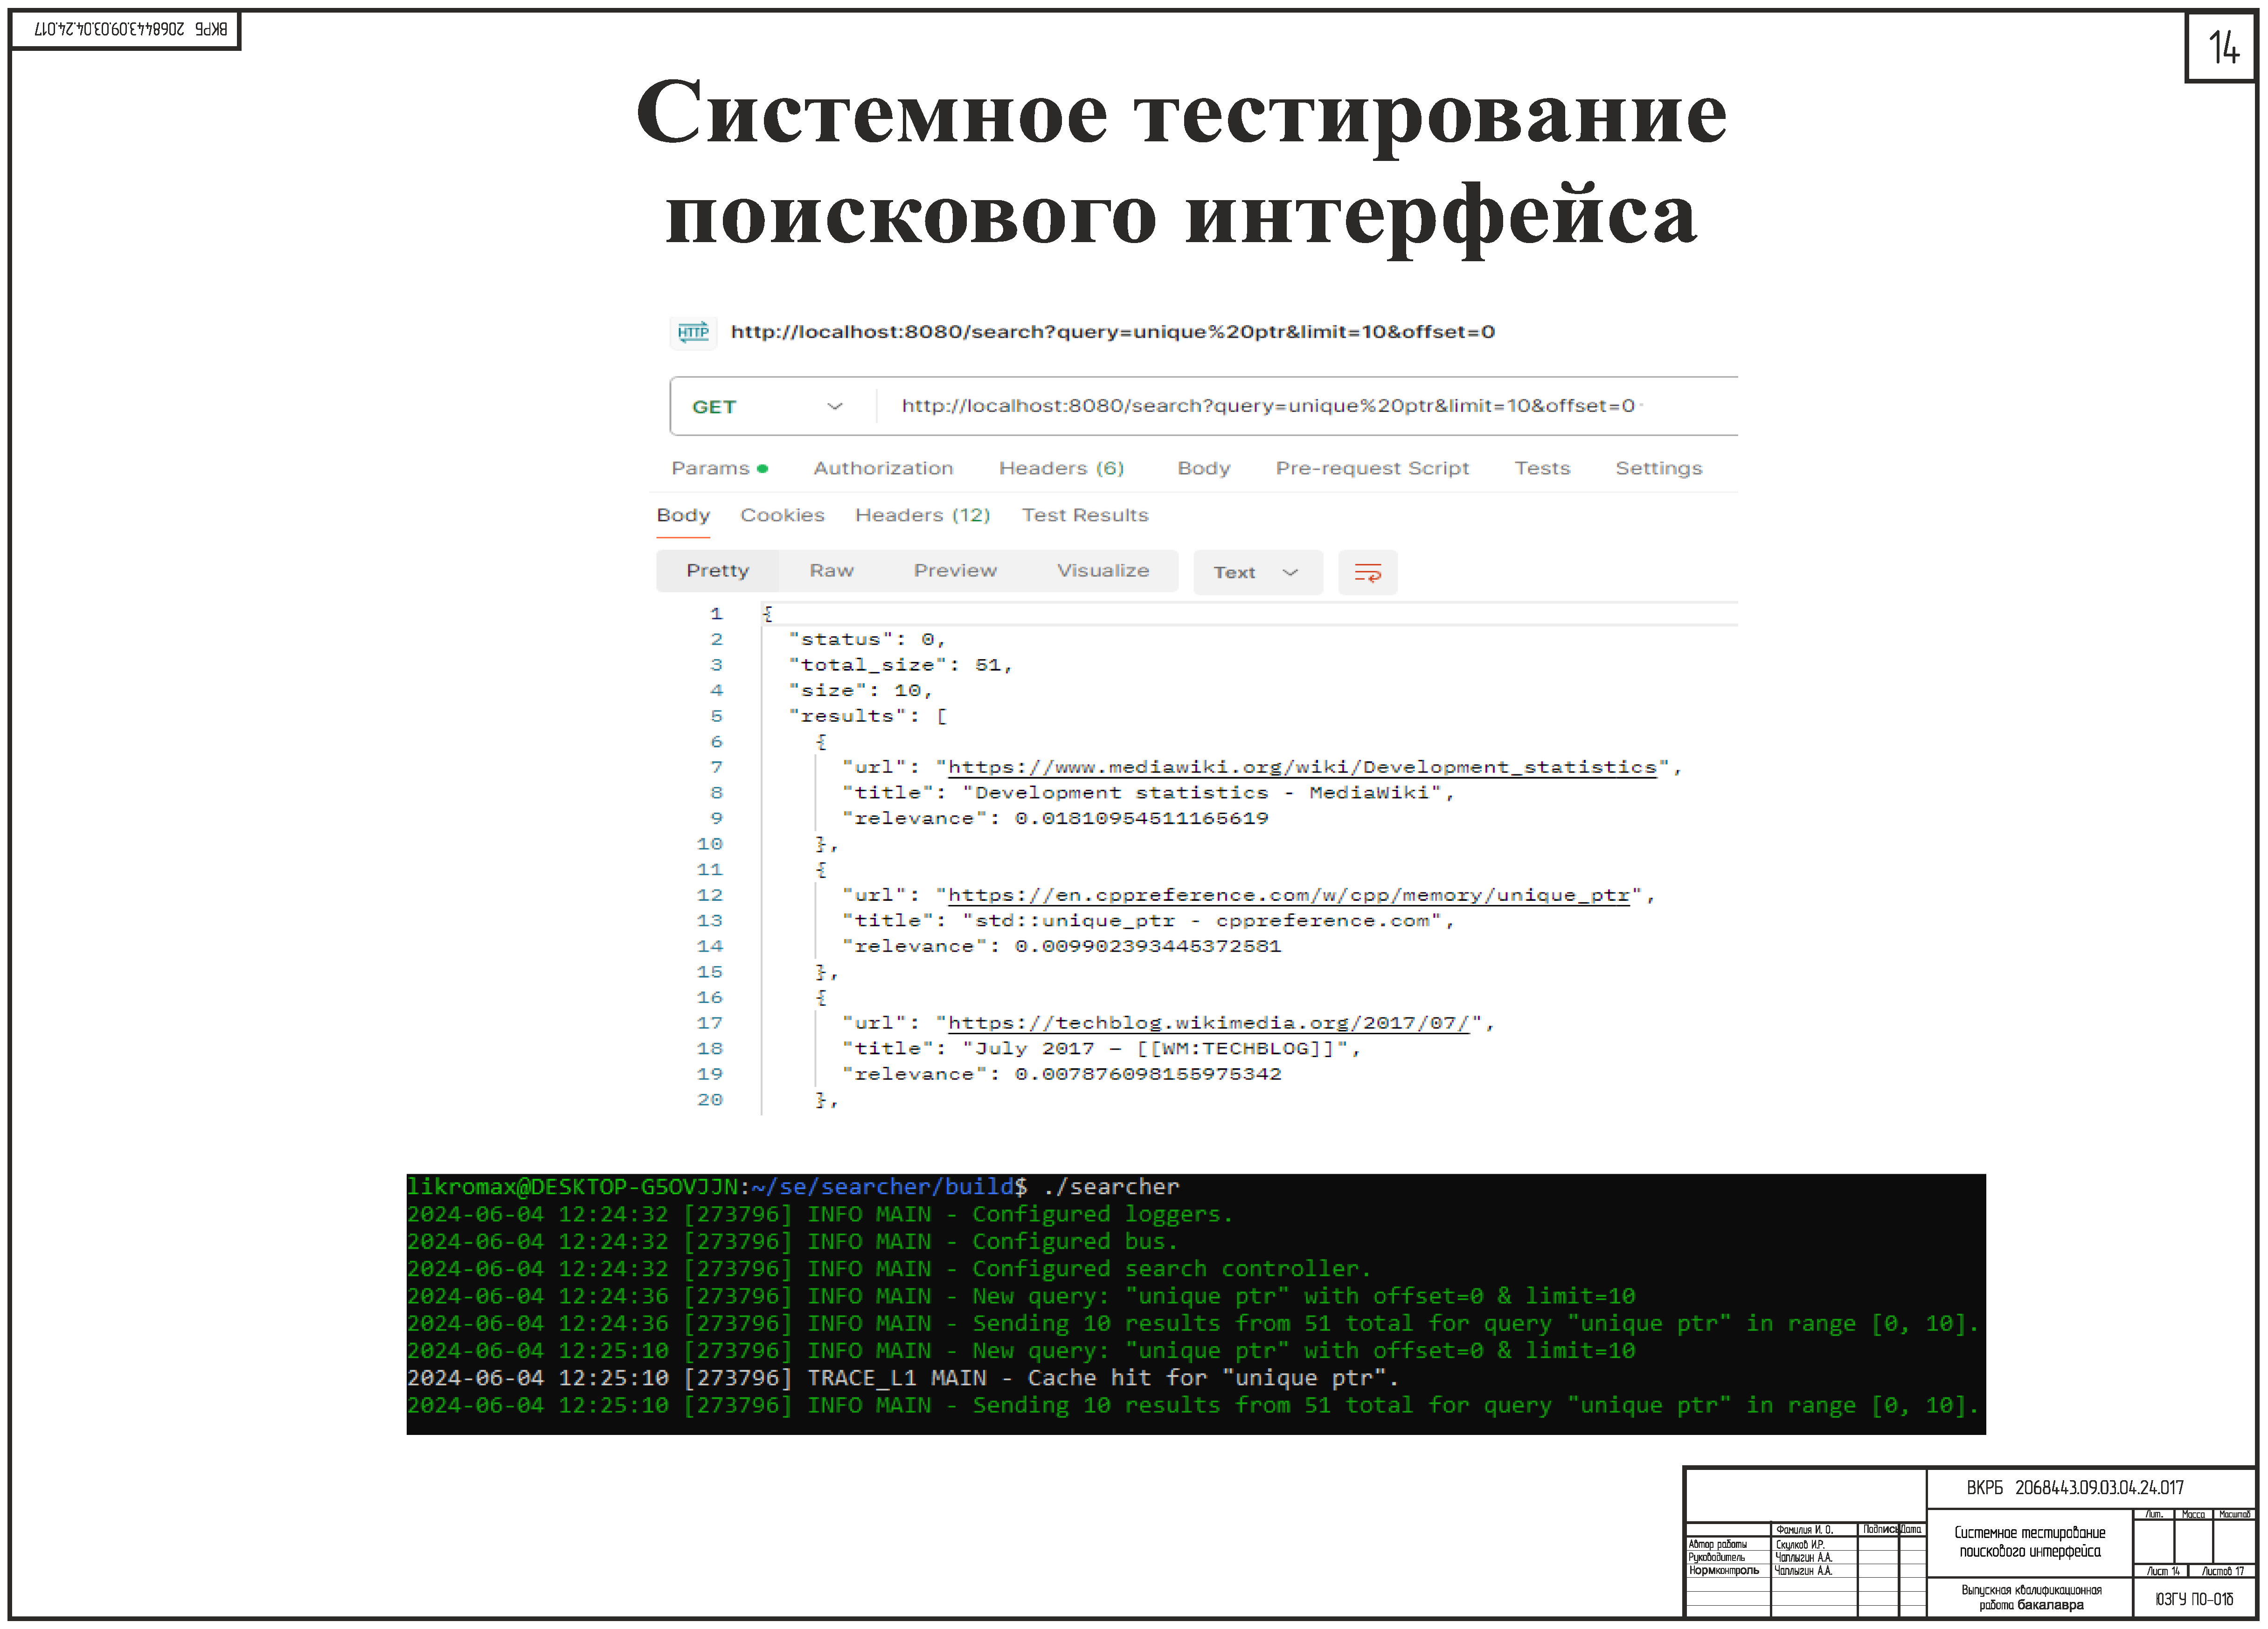
\includegraphics[width=0.82\linewidth]{posters/pts.eps}
    \заголовок{Системное тестирование поискового интерфейса}
    \label{pts:image}      
\end{плакат}

\begin{плакат}
    
\includegraphics[width=0.82\linewidth]{posters/ptl.eps}
    \заголовок{Системное тестирование сборщика журналируемой информации}
    \label{ptl:image}      
\end{плакат}

\begin{плакат}
    
\includegraphics[width=0.82\linewidth]{posters/ptw.eps}
    \заголовок{Системное тестирование веб-интерфейса}
    \label{ptw:image}      
\end{плакат}

\begin{плакат}
    
\includegraphics[width=0.82\linewidth]{posters/p6.eps}
    \заголовок{Заключение}
    \label{p6:image}      
\end{плакат}

\end{landscape}}\fi
\ifПрактика{}\else{\appendix{Фрагменты исходного кода программы}

crawler.cpp
\lstinputlisting[language=C++, frame=none]{code/crawler.cpp}

crawler.sql
\lstinputlisting[language=SQL, frame=none]{code/crawler.sql}

indexer.cpp
\lstinputlisting[language=C++, frame=none]{code/indexer.cpp}

indexer.sql
\lstinputlisting[language=SQL, frame=none]{code/indexer.sql}

search\_controller.cpp
\lstinputlisting[language=C++, frame=none]{code/searcher.cpp}

searcher.sql
\lstinputlisting[language=SQL, frame=none]{code/searcher.sql}

logs\_collector.cpp
\lstinputlisting[language=C++, frame=none]{code/logger.cpp}

logger.sql
\lstinputlisting[language=SQL, frame=none]{code/logger.sql}

\ifВКР{
\newpage
\addcontentsline{toc}{section}{На отдельных листах (CD-RW в прикрепленном конверте)}
\begin{center}
\textbf{Место для диска}
\end{center}
}\fi}\fi
\end{document}

